\documentclass[11pt]{article}

%\usepackage{fancyhdr}
\usepackage{graphicx}
\usepackage{amssymb,amsmath,stackrel}
\usepackage{lscape}
\usepackage[colorlinks]{hyperref}
\usepackage{subeqnarray}
\usepackage{chemfig}
\usepackage{subfigure}
\usepackage{subfigmat}
\usepackage{cite}
\usepackage{subeqnarray}
\usepackage[bf,small]{caption}
\usepackage{slashbox}
\usepackage{enumitem}

\usepackage[nameinlink, capitalize]{cleveref}
\crefname{table}{Tab.}{Tabs.}
\crefname{section}{Sec.}{Secs.}
%\crefname{figure}{Figure}{Figures}

\usepackage{chngcntr}
\counterwithin{figure}{section}
\counterwithin{table}{section}
\counterwithin{equation}{section}
\makeatletter
\renewcommand\p@subfigure{\thefigure}
\makeatother

\usepackage{indentfirst}
\usepackage{pdfpages}

\usepackage{pifont}

\renewcommand{\contentsname}{\LARGE Contents}
\newcommand{\crefrangeconjunction}{--}

%%%%%%%%%%%%%%%%%%%%%%%%%%%%%%%%%%%%%%%%%%%%%%%%%%%%%%%%%%%%%%%%%
\RequirePackage{calc}
%%%%%%%%%%%%%%%%%%%%%%%%%%%%%%%%%%%%%%%%%%%%%%%%%%%%%%%%%%%%%%%%%

\addtolength{\voffset}{-1in}
\addtolength{\hoffset}{-1in}
\setlength{\topmargin}{2.5cm}
\setlength{\oddsidemargin}{2.5cm}
\setlength{\evensidemargin}{2.5cm}
\setlength{\textwidth}{\paperwidth - 5cm}
\setlength{\textheight}{\paperheight - 8cm}
\setlength{\footskip}{36pt}
\setlength{\marginparsep}{0.5cm}
\setlength{\marginparwidth}{1.5cm}
\setlength{\headheight}{0.6 in}
\setlength{\headsep}{0.2 in}

\usepackage{floatrow}
\newfloatcommand{capbtabbox}{table}[][1.4\FBwidth]
\setcounter{secnumdepth}{4}
\setcounter{tocdepth}{3}
\renewcommand{\refname}{\vspace{-8mm}}

\captionsetup[figure]{labelsep=quad}
\captionsetup[table]{labelsep=quad}
%\renewcommand\tablename{Tab.}

\usepackage{chemfig}

\graphicspath{{Figures/}}

%%%%%%%%%%%%%%%%%%%%%%%%%%%%%%%%%%%%%%%%%%%%%%%%%%%%%%%%%%%%%%%%%
\title{-- Course Reader --\\
ME 257/357: Propulsion System and Gas-Turbine Analysis\\
{\small \it(Version 2.0)}}
\author{Matthias Ihme\\
Stanford University}
\setcounter{section}{0}
%%%%%%%%%%%%%%%%%%%%%%%%%%%%%%%%%%%%%%%%%%%%%%%%%%%%%%%%%%%%%%%%%

\begin{document}
\input{abbrevs}

\maketitle
\vfill
\begin{center}
\textcopyright~mihme@stanford.edu
\end{center}
\thispagestyle{empty}

%%%%%%%%%%%%%%%%%%%%%%%%%%%%%%%%%%%%%%%%%%%%%%%%%%%%%%%%%%%%%%%%%
\newpage
\setcounter{page}{1}
\pagenumbering{roman}
\tableofcontents

%%%%%%%%%%%%%%%%%%%%%%%%%%%%%%%%%%%%%%%%%%%%%%%%%%%%%%%%%%%%%%%%%
\newpage
\setcounter{page}{1}
\pagenumbering{arabic}

%%%%%%%%%%%%%%%%%%%%%%%%%%%%%%%%%%%%%%%%%%%%%%%%%%%%%%%%%%%%%%%%%
\section*{\label{SEC_REFERENCES}Recommended Reading}
%%%%%%%%%%%%%%%%%%%%%%%%%%%%%%%%%%%%%%%%%%%%%%%%%%%%%%%%%%%%%%%%%
\addcontentsline{toc}{section}{Recommended Reading}

Since this course covers material from different subject areas (including aerodynamics, thermodynamics, gas turbines, and specialized topics on internal combustion engines and rocket-propulsion), we are relying on different references. Below is a list of complementary reading material for this course; all books are on reserve at the library:
\begin{itemizePacked}
 \item Thermodynamics:
  \begin{itemizePacked}
   \item Cengel \& Boles: Thermodynamics: An Engineering Approach, McGraw-Hill~\cite{CENGEL_BOLES_BOOK2010};
   \item Reynolds \& Perkins: Engineering Thermodynamics, McGraw-Hill~\cite{REYNOLDS_PERKINS_BOOK1977}.
  \end{itemizePacked}
 \item Aerodynamics:
  \begin{itemizePacked}
   \item Anderson: Introduction to Flight, McGraw-Hill~\cite{ANDERSON_INTRO_TO_FLIGHT_BOOK2012};
   \item	Anderson: Modern Compressible Flow, McGraw-Hill~\cite{ANDERSON_MODERN_COMPRESS_FLOWS_BOOK2004}.
  \end{itemizePacked}
 \item	Gas Turbine Engines
  \begin{itemizePacked}
   \item    Mattingly: Elements of Propulsion: Gas Turbines and Rockets, AIAA Ed. Series.~\cite{MATTINGLY_BOOK2006} (Recommended Text)
   \item    Saravanamuttoo, Rogers, Cohen, \& Straznicky: Gas Turbine Theory, Pearson~\cite{SARAVANAMUTTOO_ROGERS_COHEN_STRAZNICKY_BOOK2008}
   \item	Hill \& Peterson: Mechanics and Thermodynamics of Propulsion, Addison-Wesley~\cite{HILL_PETERSON_BOOK1992};
   \item	Lefebvre: Gas Turbine Combustion, Taylor \& Francis~\cite{LEFEBVRE_BOOK1999};
   \item	Farokhi: Aircraft Propulsion, Wiley~\cite{FAROKHI_BOOK2009};
   \item	Cumpsty: Jet Propulsion -- A Simple Guide to the Aerodynamic and Thermodynamic Design and Performance of Jet Engines, Cambridge University Press~\cite{CUMPSTY_JET_BOOK1997};
   \item	Rolls Royce: The Jet Engine -- A Complete Overview of the Modern Gas Turbine~\cite{ROLLS_ROYCE_BOOK}.
   \item    Dixon \& Hall: Fluid Mechanics and Thermodynamics of Turbomachinery, Butterworth-Heinemann (also available as online resource: \url{http://www.sciencedirect.com/science/book/9780124159549})
   \item    Online resource to Jane's aero engines: \url{https://janes.ihs.com}
  \end{itemizePacked}
   \item	Internal Combustion Engines:
  \begin{itemizePacked}
   \item	Heywood: Internal Combustion Engine Fundamentals, McGraw-Hill~\cite{HEYWOOD_BOOK1988};
   \item	Stone: Introduction to Internal Combustion Engines, Palgrave MacMillan~\cite{STONE_BOOK1999};
   \item	Lumley: Engines -- An Introduction, Cambridge University Press~\cite{LUMLY_BOOK1999}.
  \end{itemizePacked}
   \item	Rocket Propulsion
  \begin{itemizePacked}
   \item	Sutton \& Biblarz: Rocket Propulsion Elements, Wiley~\cite{SUTTON_BIBLARZ_BOOK2010};
   \item    Huzel \& Huang: Modern Engineering for Design of Liquid-Propellant Rocket Engines, 
            American Institute of Aeronautics and Astronautics~\cite{HUZEL_HUANG_BOOK1992}.
  \end{itemizePacked}
\end{itemizePacked}
\clearpage
%%%%%%%%%%%%%%%%%%%%%%%%%%%%%%%%%%%%%%%%%%%%%%%%%%%%%%%%%%%%%%%%%
\section*{\label{SEC_NOMENCLATURE}Nomenclature}
%%%%%%%%%%%%%%%%%%%%%%%%%%%%%%%%%%%%%%%%%%%%%%%%%%%%%%%%%%%%%%%%%
\addcontentsline{toc}{section}{Nomenclature}

\begin{table}[!h!]
  \begin{center}
    \begin{tabular}{|c@{\hspace{0.5cm}}p{6.5cm}cc|}\hline
      {{Symbol}} & {{Description}} &
      {{Value}} &{{Units}}\\ \hline \hline

      $H$ & Enthalpy & - & J \\
      $M$ (or $W$) & Molecular weight & - & ${\mbox{g}}/{\mbox{mol}} $\\
      $N_A$ & Avogadro constant & $6.022\times10^{23}$ & $ \mbox{mol}^{-1} $\\
      $N$ & Number of particles/molecules & - & - \\
      $Q$ & Heat & - & J \\
      $R$ & Gas constant & - & ${\mbox{J}}/({\mbox{g}\,\mbox{K}})$ \\
      $S$ & Entropy & - & J/K \\
      $T$ & Temperature & - & $ \mbox{K} $\\
      $T$ & Thrust & - & $ \mbox{N} $\\
      $U$ & Internal energy & - & J \\
      $V$ & Volume & - & $ \mbox{m}^3 $\\
      $V_{\rm{m}}=V/n$ & Molar volume & - & $ \mbox{m}^3/\mbox{mol} $\\
      $X_i$ & Mole fraction of species $i$ & - & - \\
      $Y_i$ & Mass fraction of species $i$ & - & - \\
      $c_{\{p,v\}}$ & Specific heat at constant \{pressure, volume\} & - & J/(kg\,K) \\
      $k_B$ & Boltzmann constant & $1.3806 \times 10^{-23}$ &		${\mbox{J}}/{\mbox{K}}$\\
      $m$ & Mass & - & $ \mbox{g} $\\
      $n$ & Number of moles & - & $ \mbox{mol} $\\
      $p$ & Pressure & - & $ \mbox{Pa} $\\
      $\uvec, u$ & Velocity & - & $ \mbox{m/s} $\\
      $\rho$ & Density & - & $ {\mbox{g}}/{\mbox{m}^3}$\\
      $\nu_i$ & Stoichiometric coefficient, mole number of species $i$ & - & - \\
      $\phi$ & (fuel-oxygen/air) equivalence ratio & - & - \\
      $\wh{\left( \cdot \right)}$ & mole-specific quantity & - & - \\
      $\left( \cdot \right)^{\prime}$ & particle-specific quantity & - & - \\
      $\cE$ & Total Energy &  - & - \\
      $\cR$ & Universal gas constant & 8.314 & ${\mbox{J}}/({\mbox{mol}\,\mbox{K}})$\\
%      $\cT$ & Torque  & - & ${\mbox{Nm}}$\\
      \hline

    \end{tabular}
  \end{center}
\end{table}
%================================================================
\clearpage
%================================================================
\section{Introduction}
%================================================================
In this course, we will conduct a propulsion design analysis by considering three different propulsion systems, namely (i) a propeller-driven internal combustion engine, (ii) a turbojet engine, and (iii) a single-stage liquid rocket engine. Performance, efficiency, and other characteristics (emissions, fuel-utilization, and noise, etc) will be investigated in the specific context of a small four-seat private aircraft (similar to the Cirrus SR-22). The aircraft is illustrated in \cref{FIG_CIRRUS} and aircraft specifications are summarized in \cref{TAB_CIRRUS_SPECS}. The primary focus of this course is on the engine design analysis of gas turbines with specific consideration of  turbojet and turbofan engines. 

%================================================================
\begin{figure}[!tbh!]
  \begin{floatrow}
    \ffigbox{\includegraphics[width=0.56\textwidth]{cirrusSR22_photo1}}{\caption{\label{FIG_CIRRUS}Cirrus SR22.}}
    \capbtabbox{
      \begin{tabular}{|lc|}
        \hline
        \multicolumn{2}{|c|}{Performance}\\\hline\hline
        Climb Rate & 6.45 m/s\\
        Max. operating altitude & 5,334 m\\
        Max. cruise speed & 340 km/h\\\hline\hline
        \multicolumn{2}{|c|}{Weight Certification}\\\hline\hline
        Max. takeoff mass & 1542 kg\\
        Empty mass     & 1021 kg\\
        Maximum load       & 521 kg\\
        Full fuel payload         & 307 kg\\\hline\hline
        \multicolumn{2}{|c|}{Wings}\\\hline\hline
        Wing span     & 11.67 m\\
        Wing area & 13.5 m$^2$\\\hline
      \end{tabular}
    }{\caption{\label{TAB_CIRRUS_SPECS}Specifications of Cirrus SR22.}}
  \end{floatrow}
\end{figure}
%================================================================

The following specific engine design concepts are of interest for aircraft engines:
\begin{itemize}
\item {Scenario 1: Internal combustion engine}
  \begin{itemize}[noitemsep,topsep=0pt]
    \item Propeller-driven IC-engine;
    \item Single six-cylinder four-stroke engine;
    \item Example: Cessna 350 Corvalis (\cref{FIG_EXAMPLE_CESSNA}); engine:  Teledyne Continental IO-550-N.
  \end{itemize}
\item {Scenario 2: Gas-turbine engine}
  \begin{itemize}[noitemsep,topsep=0pt]
    \item Turbo-fan engine;
    \item Two-stage compressor/turbine;
    \item Example: Honda HA-420 HondaJet (\cref{FIG_EXAMPLE_HONDA}); engine: GE Honda HF120.
  \end{itemize}
\item {Scenario 3: Rocket-propelled engine}
  \begin{itemize}[noitemsep,topsep=0pt]
    \item Single-stage rocket booster;
    \item Fuels: solid, liquid, hybrid fuels;
    \item Example: Messerschmitt Me 163 (\cref{FIG_EXAMPLE_ME163}); engine: HWK 109Ð509.
  \end{itemize}
\end{itemize}

%==============================================================================
\begin{figure}[!tbh!]
  \begin{center}
  \begin{subfigmatrix}{1}
   \subfigure[\label{FIG_EXAMPLE_CESSNA}Cessna 350 Corvalis.]{\includegraphics[width = 0.45\textwidth,clip=]{cessna}}
   \subfigure[\label{FIG_EXAMPLE_HONDA}Honda HA-420 HondaJet.]{\includegraphics[width = 0.45\textwidth,clip=]{HondaJet_Side}}
   \subfigure[\label{FIG_EXAMPLE_ME163}Messerschmitt ME-163 Komet.]{\includegraphics[width = 0.45\textwidth,clip=]{Me163b2}}
  \end{subfigmatrix}
  \caption{\label{FIG_EXAMPLE}Examples of different aircraft propulsion systems: (a) propeller-driven IC-engine: Cessna 350 Corvalis, (b) turbofan engine: Honda HA-420 HondaJet, and (c) rocket-engine: Messerschmitt ME-163 Komet.}
  \end{center}
\end{figure}
%==============================================================================
\vspace*{1in}


\clearpage
%%%%%%%%%%%%%%%%%%%%%%%%%%%%%%%%%%%%%%%%%%%%%%%%%%%%%%%%%%%%%%%%%
\section{Aerodynamics and Aircraft Performance}
%%%%%%%%%%%%%%%%%%%%%%%%%%%%%%%%%%%%%%%%%%%%%%%%%%%%%%%%%%%%%%%%%
This section provides basic theoretical understanding about the aircraft performance analysis. Using this theory will allow us to evaluate basic requirements for engine design analysis, including thrust, take-off and landing, and cruise performance. To link basic thrust requirements to the engine performance, we will then derive the thrust equation and propeller theory to determine engine performance requirements. 

%%%%%%%%%%%%%%%%%%%%%%%%%%%%%%%%%%%%%%%%%%%%%%%%%%%%%%%%%%%%%%%%%
\subsection{Aerodynamics: Drag, Lift, and Airfoil Theory}
%%%%%%%%%%%%%%%%%%%%%%%%%%%%%%%%%%%%%%%%%%%%%%%%%%%%%%%%%%%%%%%%%
The aerodynamic analysis closely follows Secs. 5 and 6 of Anderson \cite{ANDERSON_INTRO_TO_FLIGHT_BOOK2012}. Here we consider an infinitely long airfoil. Forces acting on the airfoil, relevant to our analysis, include the lift and drag (see \cref{FIG_AIRFOIL}). 

%================================================================
\begin{figure}[!h!]
\begin{center}
  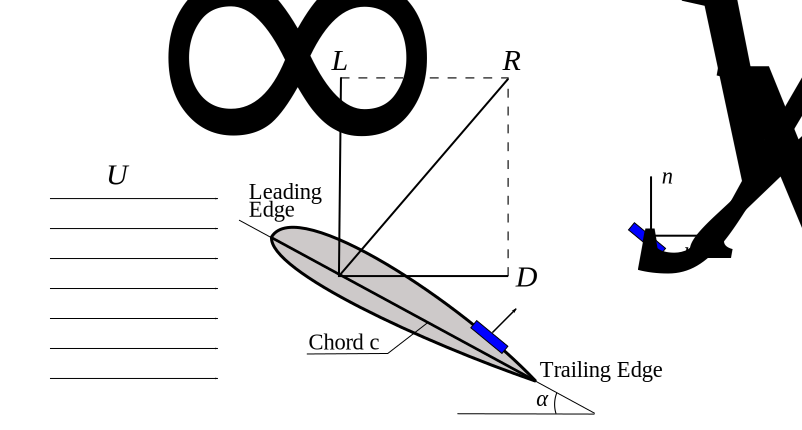
\includegraphics[scale =0.56]{airfoilDiagram}
  \caption{\label{FIG_AIRFOIL}Forces on an airfoil with $U_\infty$: free-stream velocity; $\alpha$ angle of attack; $L$ lift force; $D$ drag force; and $c$: chord.}
\end{center}
\end{figure}
%================================================================

The {\it lift force} is defined as the force on an airfoil acting in the perpendicular direction to flight path (neglecting viscous stress contributions):
\begin{equation}
  \begin{split}
    L =& - \oint p\nvec_y\cdot d \Avec\\
     =& \left.\int^c_0 p \nvec_y\cdot d \Avec\right|_\text{lower side} - \left.\int^c_0 p \nvec_y\cdot d \Avec\right|_\text{upper side} \, \text{.}
  \end{split}
\end{equation}
The {\it{lift coefficient}} is defined as
\begin{equation}
  C_L = \f{L}{q_\infty S} \, \text{,}
\end{equation}
where the dynamic pressure $q_\infty$ is defined as
\begin{equation}
   q_\infty = \f{1}{2}\rho_\infty U^2_\infty \, \text{.}
\end{equation}
Similarly, we can also define the {\it sectional lift coefficient}
\begin{equation}
  c_l = \f{l}{q_\infty c} \, \text{,}
\end{equation}
where $l$ is the lift per unit length, and $c$ is the chord.

%================================================================
\begin{figure}[!b!]
  \begin{center}
    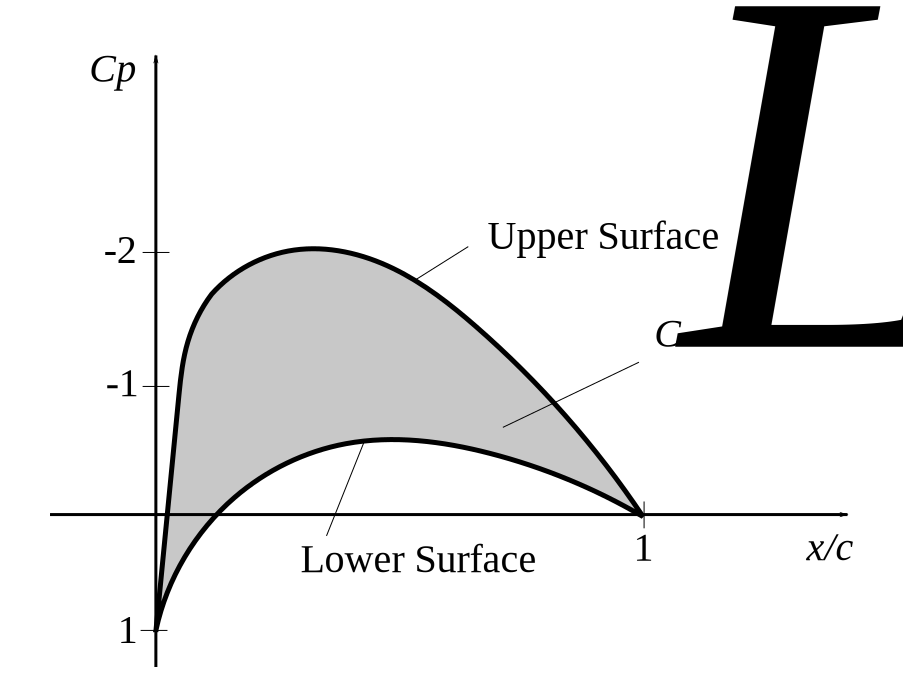
\includegraphics[width=0.52\textwidth]{pressureCoeffCurve}
    \caption{\label{FIG_PRESSURE_DISTRIBUTION}Pressure distribution over airfoil. Note that the area confined between lower and upper pressure curve is equal to $C_L$.}
  \end{center}
\end{figure}
%================================================================

Similarly, the {\it drag force} is the force on an airfoil acting in the parallel direction to the flight path (neglecting viscous stress contributions):
\begin{equation}
  \begin{split}
    D =& - \oint p\nvec_x\cdot d \Avec\\
       =& \left.\int^c_0 p \nvec_x\cdot d \Avec\right|_\text{lower side} - \left.\int^c_0 p \nvec_x\cdot d \Avec\right|_\text{upper side} \, \text{.}
  \end{split}
\end{equation}
The {\it{drag coefficient}} and {\it sectional drag coefficient} are defined as:
\begin{equation}
  C_D = \f{D}{q_\infty S} \quad \text{and} \quad c_d = \f{d}{q_\infty c} \,.
\end{equation}

For completeness, we also introduce the {\it pressure coefficient} $C_p$: 
\begin{equation}
  \label{EQ_CP_CURVE}
  C_p = \f{p-p_\infty}{q_\infty} \,.
\end{equation}
A typically pressure distribution over an airfoil is illustrated in \cref{FIG_PRESSURE_DISTRIBUTION}. The steady Bernoulli equation, $p+q=\text{const}$ (with $q=\f{1}{2}\rho U^2$), allows us to qualitatively rationalize the airfoil pressure distribution.

Note that lift and drag forces are functions of operating conditions and the airfoil geometry (see \cref{FIG_LIFT_CURVE}). This dependence can be written in terms of the following non-dimensional groups
\begin{equation}
  L = f(\alpha, \M_{\infty}, \Re, \ldots) \, \text{,}
\end{equation}
with $\alpha$ the angle of attack, $\M_\infty$ the free-stream Mach-number, and $\Re$ the Reynolds number (defined with respect to the chord-length).

%================================================================
\begin{figure}[!h!]
  \begin{center}
    \includegraphics[width=0.68\textwidth]{liftCurve}
    \caption{\label{FIG_LIFT_CURVE}Airfoil lift curve.}
  \end{center}
\end{figure}
%================================================================

From thin airfoil theory \cite{ANDERSON_INTRO_TO_FLIGHT_BOOK2012} with the assumptions (i) $\M_\infty\ll 1$ and (ii) $\Re\to\infty$ (inviscid), we can relate the lift-coefficient to the angle of attack:
\begin{equation}
  c_l = a_0(\alpha-\alpha_0)\;,
\end{equation}
where
\begin{equation}
  a_0 = \f{\p c_l}{\p \alpha} = 2\pi \, \text{.}
\end{equation}

\begin{figure}[!h!]
  \begin{center}
    \includegraphics[width=0.68\textwidth]{thin_airfoil}
    \caption{\label{FIG_THIN_AIRFOIL}Thin airfoil and vortex sheet.}
  \end{center}
\end{figure}

\Cref{FIG_THIN_AIRFOIL} shows a thin airfoil with vortex sheet place along the camber line. The distance measured along the camber line is denoted by s. The shape of the camber line is given by $z = z(x)$. $U_\infty$ is the free stream velocity, with the angle of attack $\alpha$. $U_{\infty, n}$ and $w^\prime(s)$ are the velocity component normal to the camber line by the free stream and the vortext sheet respectively. Assuming that the camber line is a streamline, then
\begin{equation}
	U_{\infty, n} + w^\prime(s) = 0 \label{eq:camber_n}
\end{equation}
at every point along the camber line.

From the geometry, and assume the thin airfoil is at small angle of attack, $\tan^{-1}\left(-dz/dx\right)\approx-dz/dx$, we have
\begin{align}
	U_{\infty, n} &= U_\infty \sin \left[ \alpha + \tan^{-1}\left(-\frac{dz}{dx}\right)\right] \\
	&= U_\infty \left(\alpha - \frac{dz}{dx}\right). \label{eq:U_inf_n}
\end{align}

For a thin airfoil, the camber line is close to the chord line, thus $w^\prime(s)\approx w(x)$. The velocity $dw$ at piont $x$ induced by the elemental vortex at point $\xi$ is given as:
\begin{equation}
	dw = -\frac{\gamma(\xi)d\xi}{2\pi(x-\xi)}.
	\label{eq:dw}
\end{equation}
$w(x)$ can be obtained by integrating \cref{eq:dw} from the leading edge $\xi=0$ to the trialing edge $\xi=c$, which is
\begin{equation}
	w(x) = -\int_0^c\frac{\gamma(\xi)d\xi}{2\pi(x-\xi)}. \label{eq:wx}
\end{equation}

Substituting \cref{eq:U_inf_n,eq:wx} into \cref{eq:camber_n} yields the \emph{fundamental equation of thin airfoil theory}, which is
\begin{equation}
	\frac{1}{2\pi}\int_0^c\frac{\gamma(\xi)d\xi}{x-\xi}=U_\infty\left(\alpha-\frac{dz}{dx}\right). \label{eq:fund_eq_thin_airfoil}
\end{equation}
For a symmetric airfoil, $dz/dx=0$, and \cref{eq:fund_eq_thin_airfoil} becomes:
\begin{equation}
	\frac{1}{2\pi}\int_0^c\frac{\gamma(\xi)d\xi}{x-\xi}=U_\infty\alpha. \label{eq:fund_eq_thin_airfoil_sym}
\end{equation}
Introduce coordinate transformation
\begin{equation}
	\xi = \frac{c}{2}(1 - \cos \theta).
\end{equation}
Note that $x$ is a fixed point which corresponds to a particular value $\theta_0$, which is
\begin{equation}
	x = \frac{c}{2}(1 - \cos \theta_0).
\end{equation}
With this, \cref{eq:fund_eq_thin_airfoil_sym} becomes
\begin{equation}
	\frac{1}{2\pi}\int_0^\pi\frac{\gamma(\theta)\sin \theta d\theta}{\cos \theta - \cos \theta_0}=U_\infty\alpha. \label{eq:fund_eq_thin_airfoil_sym2}
\end{equation}
From the mathematical theory of integral equations,
\begin{equation}
	\gamma(\theta) = 2 \alpha U_\infty \frac{1 + \cos \theta}{\sin \theta}.
\end{equation}
Note that $\gamma(\theta)$ satisfies the Kutta condition
\begin{equation}
	\lim_{\theta\rightarrow\pi}\gamma(\theta)=2 \alpha U_\infty \frac{-\sin \pi}{\cos \pi} = 0.
\end{equation}
Integrating $\gamma(\xi)$ from $0$ to $c$ yields the total circulation around the airfoil, which is
\begin{align}
	\Gamma &= \int_0^c \gamma(\xi)d\xi \\
		&= \frac{c}{2}\int_0^\pi \gamma(\theta)\sin(\theta)d\theta \\
		&= \pi \alpha c U_\infty.
\end{align}
The lift per unit span is
\begin{equation}
	L = \rho_\infty U_\infty \Gamma = \pi \alpha c \rho_\infty U_\infty^2.
\end{equation}
The lift coefficient is then
\begin{equation}
	c_l = \frac{L}{q_\infty c} = \frac{\pi \alpha c \rho_\infty U_\infty^2}{\frac{1}{2}\rho_\infty U_\infty^2 c} = 2\pi \alpha.
\end{equation}
This yields the theoretical lift slope, which is
\begin{equation}
	a_0 = \frac{\partial c_l}{\partial \alpha} = 2\pi.
\end{equation}

The lift, drag and pressure-coefficients are typically obtained from measurements or computations of an ``infinite wing span'', meaning that there are no losses due to the  finite wing-span considered. To account for finite-wing effects due to the {\it induced drag} (i.e. pressure difference across wing tip and wing-tip vortices), we can separate the drag coefficient into two contributions:
\begin{equation}
  \label{EQ_CD_RELATION}
  \underbrace{C_D}_{\text{Total Drag}} = \underbrace{C_{D,0}}_{\text{Profile Drag}} + \underbrace{C_{D,i}}_{\text{Induced Drag}} \, \text{,}
\end{equation}
where the {\it profile drag} consists of contributions from (i) skin friction, (ii) pressure drag, and (iii) flow-separation. The downwash due to tip-vortex-generation contributes to the induced drag. Another induced-drag contribution, that we typically neglect in our analysis, is the {\it wave drag}, which becomes relevant for transonic and supersonic flight conditions. 
       
For the specific case of an elliptic lift distribution, we can employ Prandtl's lifting-line theory to find an analytic expression that relates $C_{D,i}$ to the lift coefficient:
\begin{equation}
  \label{EQ_CD_CL_RELATION}
  C_{D,i} = \f{C^2_L}{\pi e AR} \, \text{,}
\end{equation}
where the aspect ratio $AR$ is expressed in terms of the wing span $b$ and wing area $S$ as:
\begin{equation}
  AR = \f{b^2}{S}=\f{b}{c} \,,
\end{equation}
and the span efficiency factor is 
\begin{equation}
e = \begin{cases} 1 & \text{for elliptic lift distribution}\\
                             <1 & \text{for general case}
      \end{cases} \, \text{.}
\end{equation}
The derivation of \cref{EQ_CD_CL_RELATION} is out of the scope for this course. Readers who are interested in the derivation of this relation may refer to Chapter 5.3 in book \emph{Fundamentals of Aerodynamics} by J. Anderson for details. Upon inserting \cref{EQ_CD_CL_RELATION} into \cref{EQ_CD_RELATION} we can derive the so-called {\it drag polar}:
\begin{equation}
C_D = C_{D,0} + \f{C^2_L}{\pi e AR} \, \text{,}
\end{equation}
which provides a relation between lift, profile drag, and total drag acting on an airfoil. A schematic of the drag polar is shown in \cref{FIG_DRAG_POLAR}.

%================================================================
\begin{figure}[!h!]
\begin{center}
 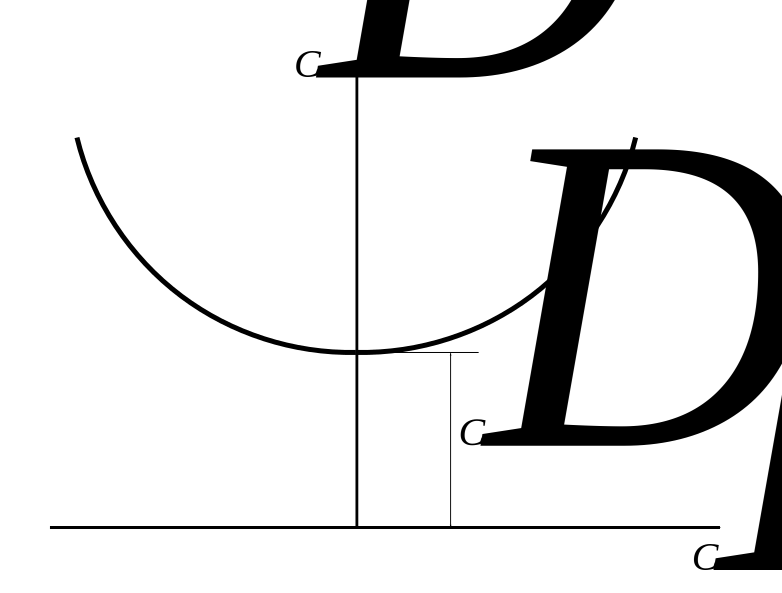
\includegraphics[width=0.46\textwidth]{dragPolar}
 \caption{\label{FIG_DRAG_POLAR}Drag polar.}
\end{center}
\end{figure}
%================================================================

%%%%%%%%%%%%%%%%%%%%%%%%%%%%%%%%%%%%%%%%%%%%%%%%%%%%%%%%%%%%%%%%%
\subsection{Aircraft Performance}
%%%%%%%%%%%%%%%%%%%%%%%%%%%%%%%%%%%%%%%%%%%%%%%%%%%%%%%%%%%%%%%%%

%%%%%%%%%%%%%%%%%%%%%%%%%%%%%%%%%%%%%%%%%%%%%%%%%%%%%%%%%%%%%%%%%
\subsubsection{Extension of Lift and Drag Coefficients}
%%%%%%%%%%%%%%%%%%%%%%%%%%%%%%%%%%%%%%%%%%%%%%%%%%%%%%%%%%%%%%%%%
This section extends the aerodynamic analysis that we performed by considering an isolated airfoil to the entire aircraft. For this, we are including additional effects and contributions due to lift and drag, arising from the airfoil, fuselage, tail flaps, landing gear, and nacelle by extending the notion of $C_D$ and $C_L$. Following this spirit, we now define $C_L$ as the {\it total lift coefficient} (that includes contributions from the above-mentioned components). The drag-coefficient of the complete aircraft is then defined as
\begin{equation}
  \label{EQ_DRAG_POLAR_AIRCRAFT}
  C_D = C_{D,0} + \f{C^2_L}{\pi e AR}
\end{equation}
where $C_{D,0}$ is the zero-lift drag coefficient of the entire aircraft (see \cref{FIG_DRAG_POLAR}), and $e$ is the Oswald efficiency factor.

The resulting drag polar of the aircraft is shown in \cref{FIG_DRAG_POLAR_AIRCRAFT}.

%================================================================
\begin{figure}[!h!]
  \begin{center}
    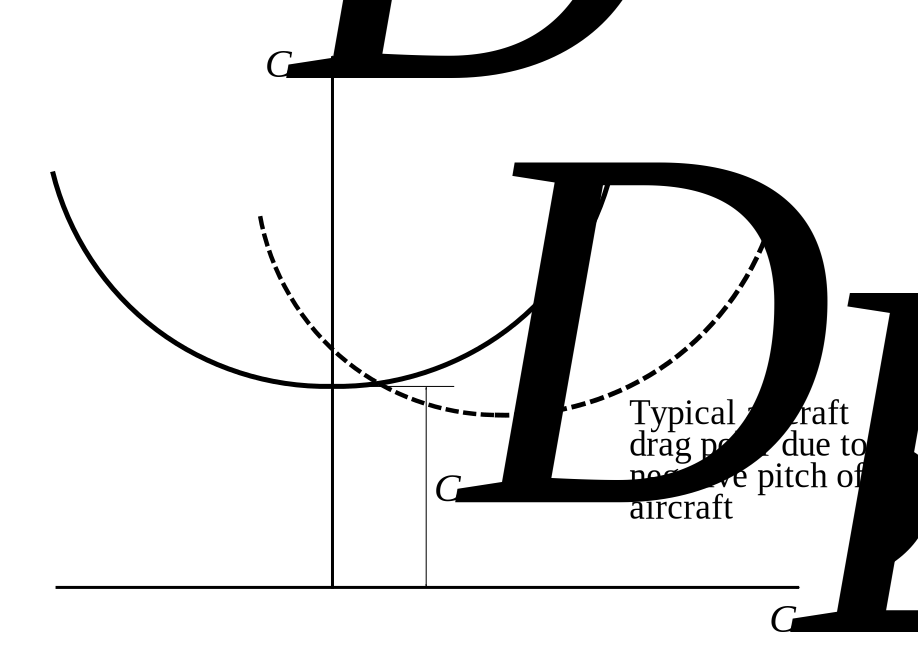
\includegraphics[width=0.56\textwidth]{dragPolarAircraft}
    \caption{\label{FIG_DRAG_POLAR_AIRCRAFT}Drag polar of aircraft, defined by \cref{EQ_DRAG_POLAR_AIRCRAFT}. Note that the minimum drag coefficient is shifted to $C_L>0$, since the zero-lift angle, $\alpha_{L=0}$, is often negative due to the downward pitch of the aircraft (a good example for this can be seen by the titled engines on an MD-80). Although rarely considered, lift is also generated at negative $C_L$ due to the fact that $\alpha_{L=0}<0$.}
  \end{center}
\end{figure}
%================================================================

%%%%%%%%%%%%%%%%%%%%%%%%%%%%%%%%%%%%%%%%%%%%%%%%%%%%%%%%%%%%%%%%%
\subsubsection{Force Balance and Thrust Requirements}
%%%%%%%%%%%%%%%%%%%%%%%%%%%%%%%%%%%%%%%%%%%%%%%%%%%%%%%%%%%%%%%%%

%================================================================
\begin{figure}[!h!]
  \begin{center}
    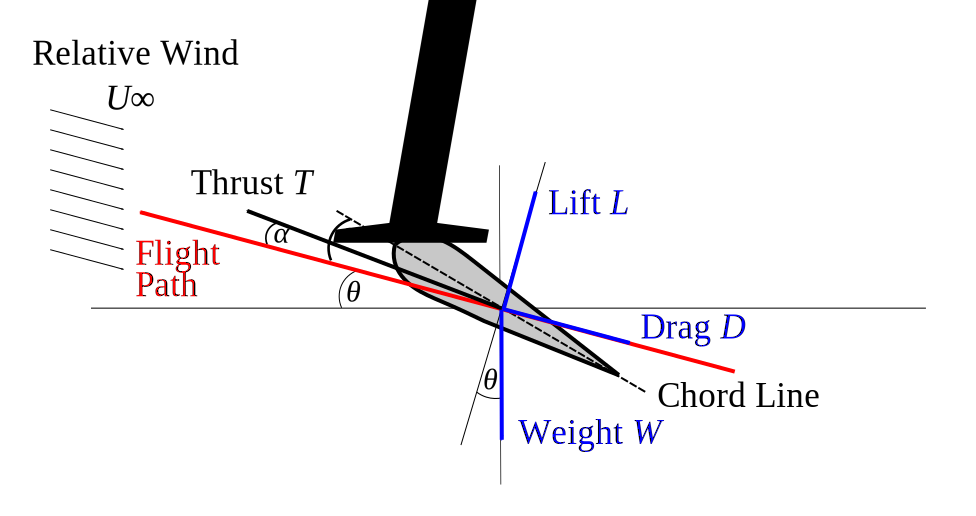
\includegraphics[width=0.7\textwidth]{forceBalanceAirfoil}
    \caption{\label{FIG_FORCE_BALANCE_AIRCRAFT}Force balance on aircraft with $\alpha$: angle-of-attack; $\theta$: inclination angle of flight path with respect to horizontal; $\alpha_T$: thrust-angle; $W$: weight; $L$: lift (perpendicular to flight path); $D$: drag (parallel to flight path); and $T$: thrust.}
  \end{center}
\end{figure}
%================================================================

From the force balance on an aircraft (see \cref{FIG_FORCE_BALANCE_AIRCRAFT}) we can set up the {\it force balance parallel to the flight path}:
\begin{equation}
   \sum_i F^\parallel_i = m\f{dU}{dt}\quad \Rightarrow\quad T\cos\alpha_T - W\sin\theta -D = m\f{dU}{dt} \, \text{,}
\end{equation}
and the {\it force balance perpendicular to the flight path}:
\begin{equation}
  \sum_i F^\perp_i = m\f{U^2}{r_c}\quad \Rightarrow\quad L+T\sin\alpha_T-W\cos\theta = m\f{U^2}{r_c} \, \text{,}
\end{equation}
where $r_c$ is the radius of the flight path (inverse of curvature of flight path).

We have some remarks and simplifications of the force balance equations:
\begin{itemize}[noitemsep,topsep=2pt]
   \item Note that $m=m(t)$, since we consume fuel during the flight:
   \begin{equation}
     m(t) = m_0 - \int_0^t \dot{m}_{fuel} dt \, \text{;}
   \end{equation}
   \item Since $\dot{m}_{fuel}$ is typically small compared to the airframe mass for airbreathing propulsion systems, we can typically neglect these effects;
   \item Often we can invoke the following sequence of simplifications:
     \begin{enumerate}[label=(\alph*),noitemsep,topsep=2pt]
       \item For the case of steady-state flight conditions, we have $d_tU = dU/dt = 0:$
         \begin{subeqnarray}
           T\cos\alpha_T - W\sin\theta -D &=& 0\\
           L+T\sin\alpha_T-W\cos\theta &=& m\f{U^2}{r_c}
         \end{subeqnarray}
       \item Thrust vector aligned with flight path ($\alpha_T=0$)
         \begin{subeqnarray}
           T - W\sin\theta -D &=& 0\\
           L-W\cos\theta &=& m\f{U^2}{r_c}
         \end{subeqnarray}
       \item Level flight: $r_c\to \infty; \theta = 0$
         \begin{subeqnarray}
           T -D &=& 0\\
           L-W &=& 0
         \end{subeqnarray}
      This reduced set of force-balance equations will be the basis for the subsequent analysis. If necessary individual assumptions can be relaxed to introduce more complexity.
      \end{enumerate}
\end{itemize}

The thrust and lift requirements for steady-level flight are:
\begin{subeqnarray}
  T = D = C_Dq_\infty S\phantom{\, \text{.}}\\
  L = W = C_Lq_\infty S\, \text{.}
\end{subeqnarray}
By taking the ratio of both equations, we have an expression for the {\it required thrust}:
\begin{equation}
  T^\ast = W\f{D}{L} = W\f{C_D}{C_L} \, \text{,}
\end{equation}
and with the  drag polar from \cref{EQ_DRAG_POLAR_AIRCRAFT}, we can write:
\begin{equation}
  T^\ast = \underbrace{C_{D,0}q_\infty S}_{\text{zero-lift drag}} + \underbrace{\f{W^2}{q_\infty S\pi e AR}}_{\text{lift-induced drag}} \, \text{.}
\end{equation}
The required thrust and thrust components vs. dynamic pressure are illustrated in \cref{FIG_THRUST_REQUIREMENT}. 

%================================================================
\begin{figure}[!b!]
\begin{center}
 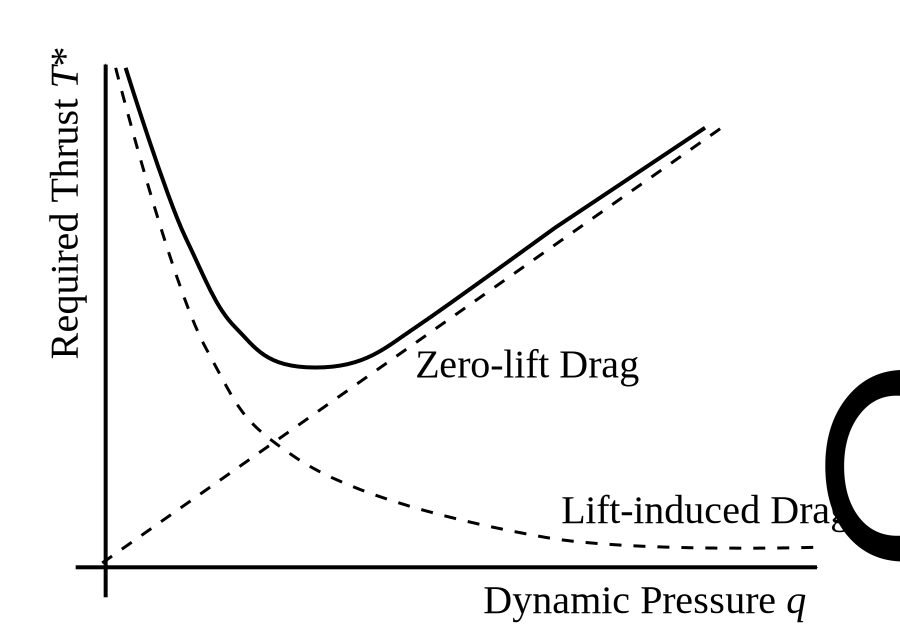
\includegraphics[width=0.55\textwidth]{requiredThrustVsDynamicPressure}
 \caption{\label{FIG_THRUST_REQUIREMENT}Required thrust vs. dynamic pressure.}
\end{center}
\end{figure}
%================================================================
 
The dependence of the thrust requirements on the angle of attack can be reconciled by introducing the expression for $C_L$ from thin airfoil theory, $C_L = a(\alpha-\alpha_0) = 2\pi (\alpha-\alpha_0)$, into the thrust equation:
\begin{equation}
  T^\ast = C_{D,0}q_\infty S + \f{[2\pi(\alpha-\alpha_0)]^2q_\infty S}{\pi e AR} \, \text{.}
\end{equation}

%%%%%%%%%%%%%%%%%%%%%%%%%%%%%%%%%%%%%%%%%%%%%%%%%%%%%%%%%%%%%%%%%
\subsubsection{Available Thrust}
%%%%%%%%%%%%%%%%%%%%%%%%%%%%%%%%%%%%%%%%%%%%%%%%%%%%%%%%%%%%%%%%%
The thrust that is provided by the engine (propeller-driven IC-engine and gas turbine, etc.) must match or exceed the required thrust. We will see later that different propulsion systems have different thrust characteristics and limitations (see \cref{FIG_THRUST_REQUIREMENT_AVAIL}) and the maximum flight speed and cruise altitude is then determined by the available thrust of the aircraft.

Note that while gas-turbines are typically rated by thrust, the performance of IC-engines is typically specified in terms of power; required flight power and thrust are related through the following expression:
\begin{equation}
  P^\ast = T^\ast U_\infty \, \text{.}
\end{equation}

%================================================================
\begin{figure}[htb]
  \begin{center}
    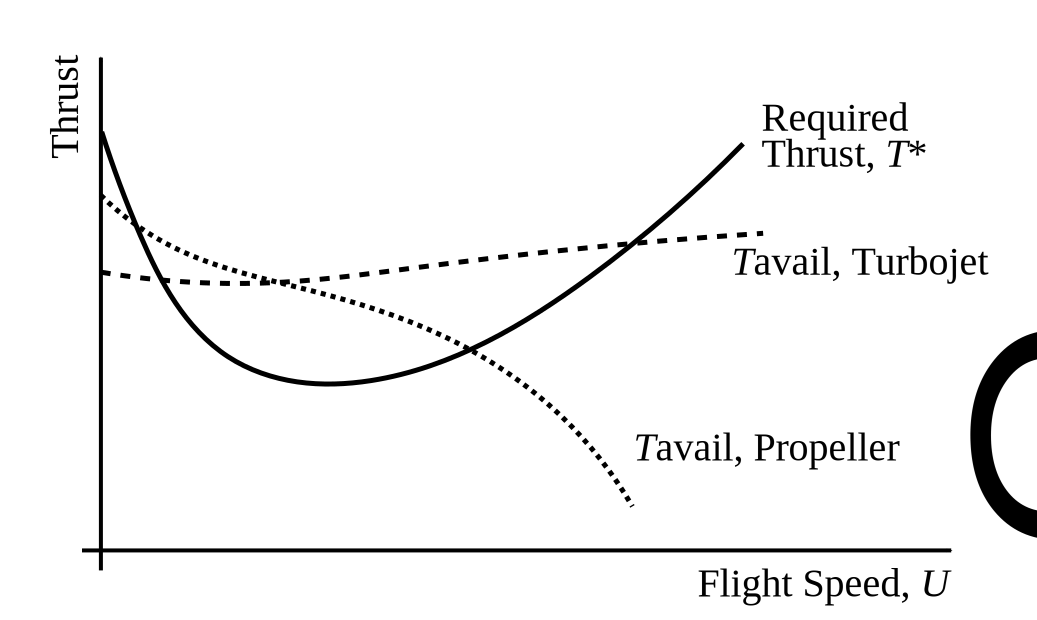
\includegraphics[width=0.56\textwidth]{thrustRequirements}
    \caption{\label{FIG_THRUST_REQUIREMENT_AVAIL}Comparison of required and available thrust for different propulsion systems.}
  \end{center}
\end{figure}
%================================================================

%%%%%%%%%%%%%%%%%%%%%%%%%%%%%%%%%%%%%%%%%%%%%%%%%%%%%%%%%%%%%%%%%
\subsection{Propulsive Thrust Generation}
%%%%%%%%%%%%%%%%%%%%%%%%%%%%%%%%%%%%%%%%%%%%%%%%%%%%%%%%%%%%%%%%%
Recall from previous sections that the required thrust is a function of speed $U_\infty$, angle of attack $\alpha$, and other flight parameters. For steady flight we  found
\begin{equation}
  \text{Required Thrust:}\quad T^\ast = C_{D,0}q_\infty S + \f{W^2}{q_\infty S \pi e AR} \, \text{.}
\end{equation}
The required thrust must be matched or exceeded by the available thrust to meet the performance requirement. The objective now is to link the required thrust to the engine thrust. For this we consider two propulsion systems, namely gas-turbine engine and propeller-driven engine (with relevance to turbofan engine).

%%%%%%%%%%%%%%%%%%%%%%%%%%%%%%%%%%%%%%%%%%%%%%%%%%%%%%%%%%%%%%%%%
\subsubsection{Thrust Equation}
%%%%%%%%%%%%%%%%%%%%%%%%%%%%%%%%%%%%%%%%%%%%%%%%%%%%%%%%%%%%%%%%%
A general equation for the thrust of airbreathing propulsion (and with some minor modifications also for rocket engines) can be derived from the conservation equations for mass and momentum. For this analysis we consider a control-volume in the coordinate system that is fixed to the engine (see \cref{FIG_CV_ANALYSIS}).

%================================================================
\begin{figure}[!h!]
\begin{center}
 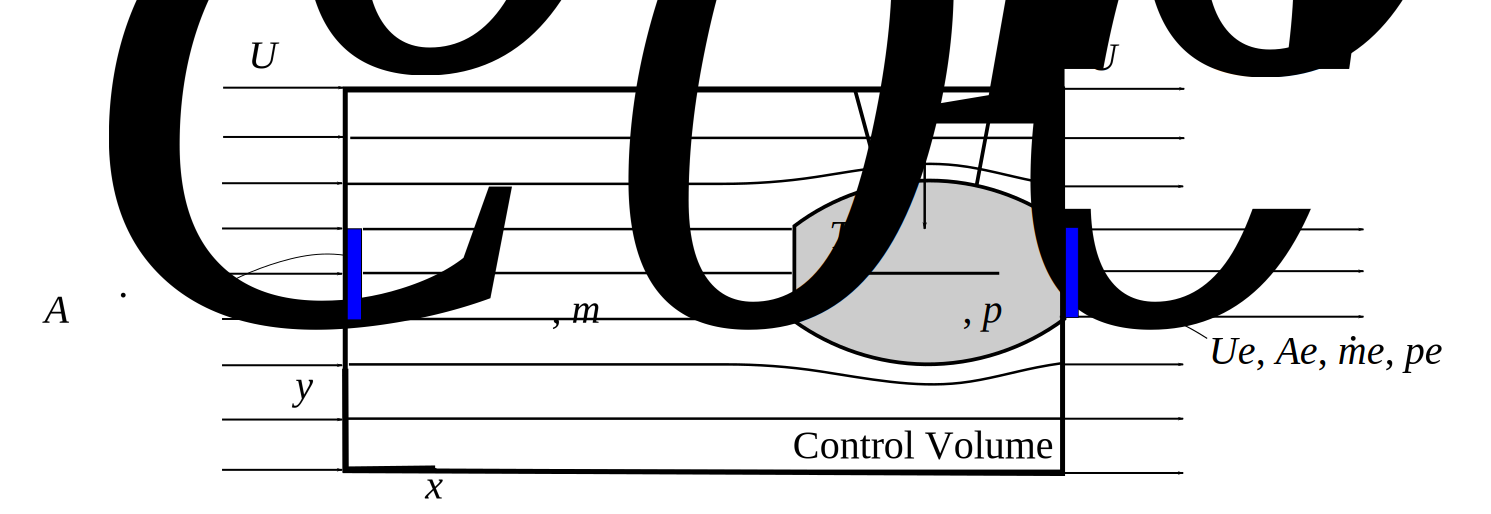
\includegraphics[width=0.88\textwidth]{thrustEquationCV}
 \caption{\label{FIG_CV_ANALYSIS}Control volume analysis for thrust equation.}
\end{center}
\end{figure}
%================================================================

Recall conservation equations
\begin{subeqnarray}
  \text{Mass:} &  \underbrace{\p_t \rho}_{\text{Rate of change}} +  \underbrace{\nabla\cdot(\rho \uvec)}_{\text{Flux of mass}} = 0\\
  \text{Momentum:} & \underbrace{\p_t (\rho\uvec)}_{\text{Rate of change}} + \underbrace{\nabla\cdot(\rho\uvec\otimes\uvec)}_{\text{Flux of momentum}} = \underbrace{-\nabla p}_{\text{Pressure force}} + \underbrace{\nabla\cdot \sigmamat}_{\text{Viscous force}} + \underbrace{\gvec}_{\text{Gravity}} + \underbrace{\fvec}_{\text{Reaction force}}
\end{subeqnarray} 
and integrate over control-volume with $d \svec$ defined to be the outward-pointing surface element
\begin{equation}
d \svec = |d\svec| \hat{\nvec} = ds \,\hat{\nvec} \, ,
\end{equation}
we will have the following form (by using the Gauss theorem):
\begin{subeqnarray}
  \p_t \int \rho dV + \oint (\rho \uvec)\cdot\wh\nvec \,d s&=& 0 \, \text{,}\\
  \p_t \int (\rho \uvec) dV + \oint(\rho \uvec) (\uvec\cdot\wh{\nvec})d s &=& - \oint p \wh\nvec\, ds + \oint \sigmamat \cdot \wh\nvec \,ds +  \int \gvec dV + \Fvec \, \text{,}
\end{subeqnarray} 
where $\Fvec = \int \fvec dV$ is the reaction force. By introducing the following assumptions:
\begin{itemizePacked}
  \item Steady state;
  \item Negligible viscous effects;
  \item Negligible gravitational forces (might become relevant for rocket-engines);
  \item Constant flow rates/properties across area cross-sections;
  \item Assume that thrust is aligned with $x$-direction,
\end{itemizePacked}
we can obtain the steady-state conservation equations for mass and momentum:
\begin{subeqnarray}
  \oint (\rho \uvec)\cdot\wh\nvec d s&=& 0 \, \text{,}\\
  \oint(\rho u_x) \uvec\cdot\wh{\nvec}d s + \oint p d S_x &=& F_x = T_U \, \text{,}
\end{subeqnarray} 
where $T_U$ is named the uninstalled thrust. By assuming that all flow-field quantities are piece-wise constant at each area-section, we can reduce the integral equations to algebraic equations:
\begin{subeqnarray}
  \text{Mass:} & -\rho_0 U_0 A_C  + \rho_eU_eA_e - \dot{m}_{F} = 0\\
  \text{$x$-Momentum:} & -\rho_0 U^2_0 A_C - p_0 A_e + \rho_e U^2_e A_e +p_e A_e = F_x
\end{subeqnarray}
and with
\begin{eqnarray}
  \dot{m}_e &=& \rho_eU_eA_e\, ,\\
  \dot{m}_A &=& \rho_0 U_0 A_C\, ,
\end{eqnarray}
where $\dot{m}_A$ is the air mass flow, we have 
\begin{subeqnarray}
\dot{m}_e = \dot{m}_A + \dot{m}_F = \dot{m}_A \left(1+\frac{\dot{m}_F}{\dot{m}_A} \right) \, , \\
F_x = \dot{m}_e U_e + \dot{m}_A U_0 + A_e (p_e - p_0) \, ,
\end{subeqnarray}
and hence we obtain the thrust equation
\begin{equation}
  \label{EQ_THRUST_EQUATION}
  F_x = T_U = \underbrace{\dot{m}_A \left[ \left(1+\f{\dot{m}_F}{\dot{m}_A}\right)U_e - U_0\right]}_{\text{Jet thrust}} + \underbrace{A_e\left(p_e - p_0\right)}_{\text{Pressure thrust}} \, \text{.}
\end{equation}

We have several remarks:
\begin{itemizePacked}
  \item Pressure thrust is typically small (zero) for subsonic aircraft and perfect expansion nozzle ($p_e = p_0$), and requires consideration for rockets and imperfectly expanded nozzles.
  \item By applying the thrust equation to propeller-flows with $\dot{m}_{F}=0$ and $p_e = p_0$, we have:
    \begin{equation}
      T_{\text{Prop}} = \dot{m}_A(U_e - U_0) \, \text{;}
    \end{equation}
  \item Applied to rockets ($\dot{m}_A = 0$) we have
   \begin{eqnarray}
     T_{\text{Rocket}} = \dot{m}_p U_e + {A_e\left(p_e - p_0\right)} \, \text{,}
   \end{eqnarray}
   where $\dot{m}_p$ is the mass flow rate of propellant.
  \item Often thrust equation derived above is referred to as {\it uninstalled thrust}, since it neglects the effects due to inlet drag and nozzle drag:
  \begin{eqnarray}
     T_I = T_U - D_{\text{Inlet}} - D_{\text{Nozzle}} \, \text{,}
  \end{eqnarray}
  where $T_I$ is the installed thrust, and the inlet and nozzle drag coefficients are defined as
  \begin{eqnarray}
     \phi_\text{Inlet} &=& \frac{D_\text{Inlet}}{T_u} \sim 0.02-0.5 \, \text{,}\\
     \phi_\text{Nozzle} &=& \frac{D_\text{Nozzle}}{T_u} \sim 0.01 \, \text{,}
  \end{eqnarray}
  and we can write
    \begin{eqnarray}
     T_I = T_U (1- \phi_{\text{Inlet}} - \phi_{\text{Nozzle}}) \, \text{.}
  \end{eqnarray} 
  \item Often thrust is given in English units,
    \begin{equation}
    T = T g_c \quad \text{and} \quad g_c = \left\{ 
         \begin{array}{r@{,\quad}l}
          1 & {\text{SI metric}}\\
          32.17 & {\frac{\text{lbm}\cdot\text{ft}}{\text{lbf}\cdot\text{s}^2}}\\
         \end{array}
         \right. \, \text{,}
    \end{equation}
    where lbm is pound mass and lbf is pound force. For $g_c$, since 1 N = 0.22482 lbf, 1~m~=~3.2808~ft and 1 kg = 2.2046 lbm, we have
    \begin{equation}
    g_c = \frac{\text{kg}\cdot\text{m}}{\text{s}^2\cdot\text{N}} = 1 = \frac{(2.2046\text{lbm})(3.2808\text{ft})}{\text{s}^2(0.22482\text{lbf})} = 32.17\, \frac{\text{lbm}\cdot\text{ft}}{\text{lbf}\cdot\text{s}^2} \, .
    \end{equation}
\end{itemizePacked}

%%%%%%%%%%%%%%%%%%%%%%%%%%%%%%%%%%%%%%%%%%%%%%%%%%%%%%%%%%%%%%%%%
\subsubsection{Thrust Equation for Turbofan Engines}
%%%%%%%%%%%%%%%%%%%%%%%%%%%%%%%%%%%%%%%%%%%%%%%%%%%%%%%%%%%%%%%%%
Classic thrust equation that we derived above only considers a single stream through the engine. However, for turbofan engines, the air stream is split into two separated streams \textendash one going through the core and the other one passing by (``bypass") and generating thrust by airflow acceleration. 

\Cref{FIG_STATION_NUMBERING} shows the control volume and definitions of the stations in a turbofan engine. Abbreviations are LPC for low-pressure compressor, HPC for high-pressure compressor, LPT for low-pressure turbine, and HPT for high-pressure turbine. Note that stations 6 and 7 are omitted and correspond to the combustor inlet/exit of the afterburner.

The bypass ratio is defined as
\begin{equation}
\beta = \frac{\dot{m}_{A\,,B}}{\dot{m}_{A\,,C}} \,,
\end{equation}
where $\dot{m}_{A\,,B}$ is the airflow through bypass and $\dot{m}_{A\,,C}$ is the airflow through core.

Assume that both streams expand to $p_e = p_0$ separately and there is no mixing among streams. Thrust equation for turbofan engine in general form is
\begin{equation}
  T = \dot{m}_{A\,,C} \left[ (1+f) U_e + \beta U_{1e} - (1+\beta) U_0 \right] + A_e (p_e - p_0) + A_{1e} (p_{1e} - p_0)\, \text{,}
\end{equation}
where $f = \dot{m}_F/\dot{m}_A$, $U_e$ is the core exit velocity, and $U_{1e}$ is the fan exit velocity.

%==============================================================
\begin{figure}[!htb!]
 \centering
    {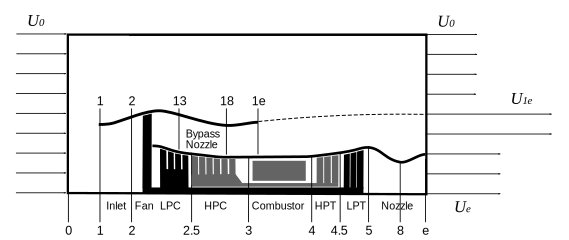
\includegraphics[width=0.9\textwidth, clip=, keepaspectratio]{turboFanEngine}}
    \caption{\label{FIG_STATION_NUMBERING}Control volume analysis for turbofan thrust equation and station numbering for a commercial twin-spool turbofan engine.}
\end{figure}
%==============================================================

%%%%%%%%%%%%%%%%%%%%%%%%%%%%%%%%%%%%%%%%%%%%%%%%%%%%%%%%%%%%%%%%%
\subsection{Fuel Consumption and Range Equation}
%%%%%%%%%%%%%%%%%%%%%%%%%%%%%%%%%%%%%%%%%%%%%%%%%%%%%%%%%%%%%%%%%
The weight of the aircraft decreases during the flight as a result of the fuel consumption. The aircraft mass can be expressed as
\begin{equation}
  m = \underbrace{m_{AF}}_{\text{Airframe mass}} + \underbrace{m_F}_{\text{Fuel mass}} \, ,
\end{equation}
where $m_{AF}$ is fixed and 
\begin{equation}
  m_F = m_{F, 0} - \int_0^t \dot{m}_F dt
\end{equation}
in which $\dot{m}_F$ is the fuel consumption rate and $m_{F,0}$ is the initial fuel mass. The rate of change of the weight of the aircraft, $W = mg$, is
\begin{equation}
  \frac{dW}{dt} = \frac{d}{dt}(mg) = - \dot{m}_F g \, .
\end{equation}
With the {\it thrust specific fuel consumption} defined as
\begin{equation}
  \text{TSFC} = \frac{\dot{m}_F}{T}
\end{equation}
where $T$ is the thrust, we have
\begin{equation}
  \frac{dW}{dt} = - \text{TFSC}\, T g\,.
\end{equation}
For level flight, we have $T = W (C_D/C_L)$ and thus
\begin{equation}
  \frac{dW}{W} = - \text{TSFC} \, \frac{C_D}{C_L} g dt\,.
\end{equation}
With the {\it endurance factor} EF defined as
\begin{equation}
\text{EF} = \frac{C_L}{C_D} \frac{1}{\text{TSFC} \,g}\,,
\end{equation}
we have 
\begin{equation}
\frac{dW}{W} = -\frac{dt}{\text{EF}}\,.
\end{equation}

Assume $C_D/C_L$ is constant, we can integrate to have the weight as a function of flight time,
\begin{equation}
  \frac{W(t)}{W_0} = \text{exp}\left(-\frac{t}{\text{EF}}\right) = \text{exp}\left(-\frac{C_D}{C_L} \text{TSFC} \, g \,t\right) \,.
\end{equation}
By using $ds = U dt$ and the {\it range factor} RF defined as 
\begin{equation}
\text{RF} = \frac{C_L}{C_D} \frac{U}{\text{TSFC} \,g}\,,
\end{equation}
we have
\begin{equation}
  \label{eqn:BRE}
  \frac{W(s)}{W_0} = \text{exp}\left(-\frac{s}{\text{RF}}\right) = \text{exp}\left(-\frac{C_D}{C_L} \frac{\text{TSFC}}{U} \, g \,s\right) \,.
\end{equation}
\Cref{eqn:BRE} is referred to as the Breguet range equation. \Cref{fig:EFRF} shows the plots of EF and RF as a function of flight Mach number and the flying altitude.

%================================================================
\begin{figure}[!b!]
  \begin{center}
    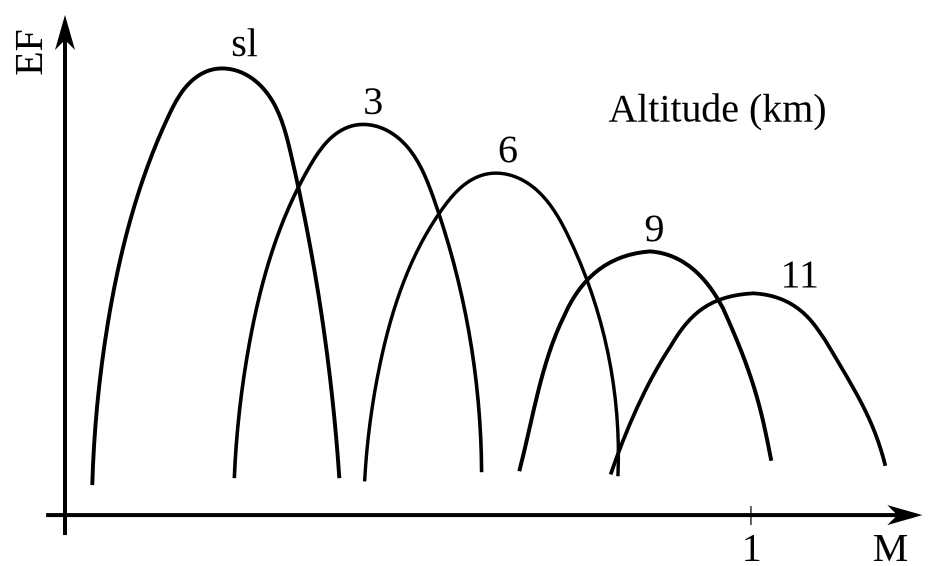
\includegraphics[width=0.48\textwidth]{EF}
    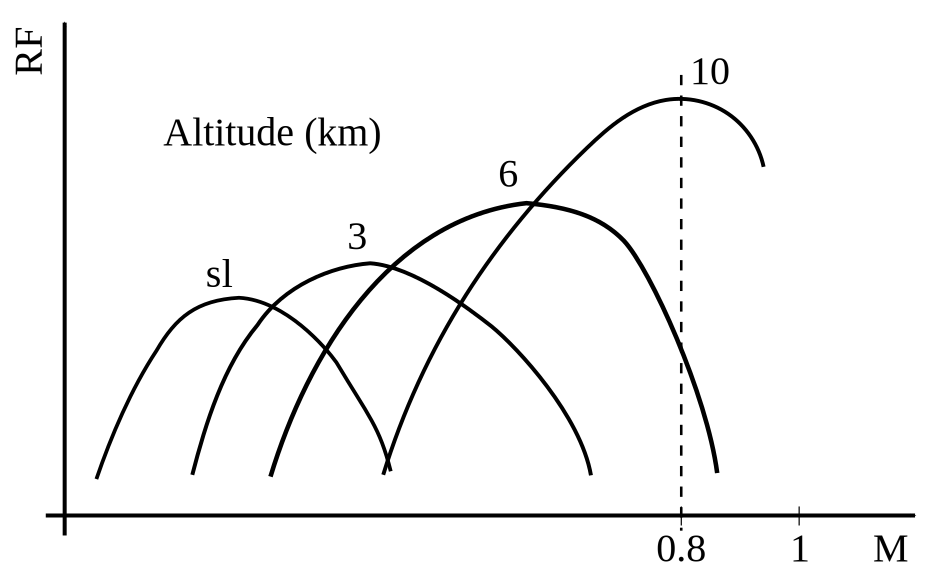
\includegraphics[width=0.48\textwidth]{RF}
    \caption{\label{fig:EFRF}Endurance factor and range factor.}
  \end{center}
\end{figure}
%================================================================

The TSFC is a function of engine, altitude and the flight Mach number. Some useful estimates for $\text{TSFC}_\text{I}$ (the subscript I means for $T_I$) are
\begin{itemizePacked}
\item High bypass-ratio turbofan engine:
  \begin{equation}
  \text{TSFC}_\text{I} = (0.4 + 0.45 \text{M}) \sqrt{\frac{T}{T_\text{ref}}} \, ;
  \end{equation}
\item LBR turbofan engine (military):
  \begin{equation}
  \text{TSFC}_\text{I} = (1.0 + 0.35 \text{M}) \sqrt{\frac{T}{T_\text{ref}}} \, ;
  \end{equation}
\item Turbojet (military):
  \begin{equation}
  \text{TSFC}_\text{I} = (1.3 + 0.26 \text{M}) \sqrt{\frac{T}{T_\text{ref}}} \, .
  \end{equation}
\end{itemizePacked}

%%%%%%%%%%%%%%%%%%%%%%%%%%%%%%%%%%%%%%%%%%%%%%%%%%%%%%%%%%%%%%%%%%
\subsection{Performance Parameters}
%%%%%%%%%%%%%%%%%%%%%%%%%%%%%%%%%%%%%%%%%%%%%%%%%%%%%%%%%%%%%%%%%%

%%%%%%%%%%%%%%%%%%%%%%%%%%%%%%%%%%%%%%%%%%%%%%%%%%%%%%%%%%%%%%%%%
\subsubsection{Thermal Efficiency}
%%%%%%%%%%%%%%%%%%%%%%%%%%%%%%%%%%%%%%%%%%%%%%%%%%%%%%%%%%%%%%%%%

%================================================================
\begin{figure}[!b!]
  \begin{center}
    \includegraphics[width=0.58\textwidth]{etaThermal}
    \caption{\label{fig:ETA_THERMAL}Evolution of thermal efficiency over time.}
  \end{center}
\end{figure} 
%================================================================

The thermal efficiency is defined to be the net rate of power output (kinetic energy) over the available thermal energy:
\begin{equation}
  \eta_\text{th} = \f{\dot{P}_\text{out}}{\dot{Q}_\text{in}} = \f{\text{Net power of engine}}{\text{Heat addition by combustion}} \,,
\end{equation}
and
\begin{equation}
  \dot{P}_\text{out} = \f{1}{2} \dot{m}_F  \left[ \left( 1+\f{\dot{m}_A}{\dot{m}_F}\right)U_e^2-U_0^2\right]\,,
\end{equation}
which is the net rate of change of kinetic energy through the engine. The heat addition is defined as:
\begin{equation}
  \dot{Q}_\text{in} = \dot{m}_F \text{LHV}\,,
\end{equation}
where LHV is the lower heating value of fuel (which considers that the water that is formed in the combustion products remains in the vapor state). With this,
the thermal efficiency can be written as:
\begin{equation}
  \eta_\text{th} = \f{1}{2 \text{LHV}} \f{\dot{m}_A}{\dot{m}_F} \left[ \left( 1+\f{\dot{m}_A}{\dot{m}_F}\right)U_e^2-U_0^2\right]\,.
\end{equation}
\Cref{fig:ETA_THERMAL} shows the thermal efficiency as a function of year.

%%%%%%%%%%%%%%%%%%%%%%%%%%%%%%%%%%%%%%%%%%%%%%%%%%%%%%%%%%%%%%%%%
\subsubsection{Propulsive Efficiency}
%%%%%%%%%%%%%%%%%%%%%%%%%%%%%%%%%%%%%%%%%%%%%%%%%%%%%%%%%%%%%%%%%
The propulsive efficiency is a measure for how efficiently the engine power is used to power the aircraft:
\begin{equation}
  \label{EQ_ETA_P}
  \eta_p = \f{\text{Propulsive power of aircraft}}{\text{Net power of engine}} = \f{\dot{P}_p}{\dot{P}_\text{out}}\,,
\end{equation}
where $P_p = T_I U_0$ (with $T_I$ being the installed thrust) is the propulsive power. With this, the propulsive efficiency can be written as:
\begin{equation}
  \begin{split}
    \eta_p &= \f{T_IU_0}{\f{1}{2}\dot{m}_A\left[ \left( 1+\f{\dot{m}_A}{\dot{m}_F}\right)U_e^2-U_0^2\right]}\;,\\
               &= \f{(1-\phi_\text{inlet}-\phi_\text{nozzle})U_0\left\{\dot{m}_A\left[ \left( 1+\f{\dot{m}_A}{\dot{m}_F}\right)U_e^2-U_0^2\right] + A_C (p_e-p_0) \right\}}{\f{1}{2}\dot{m}_A\left[ \left( 1+\f{\dot{m}_A}{\dot{m}_F}\right)U_e^2-U_0^2\right]}\,.
  \end{split}
\end{equation}
For the case of (i) a perfectly expanded nozzle, (ii) $\dot{m}_F/\dot{m}_A=f \rightarrow 0$, and (iii) $T_I \rightarrow T_U$ with $\phi_\text{inlet} = 0$ and $\phi_\text{nozzle} = 0$, \cref{EQ_ETA_P} reduces to:
\begin{equation}
\label{eqn:etaPropulsive}
  \eta_p = \f{2U_0}{U_e+U_0} = \f{2}{1+\f{U_e}{U_0}}\,.
\end{equation}
\Cref{fig:ETA_PROPULSIVE} shows the propulsive as a function of $U_e / U_0$. From this figure it can be seen that we require $U_e\to U_0$ to achieve a maximum propulsive efficiency of unity. However, at this condition, no thrust is generated. Conditions with $U_e/U_0<1$ correspond to a wind generator in which we extract work from the air to generate power, and a windmill is a typical example for this.

%================================================================
\begin{figure}[!htb!]
  \begin{center}
    \includegraphics[width=0.56\textwidth]{etaPropulsive}
    \caption{\label{fig:ETA_PROPULSIVE}Propulsive efficiency.}
  \end{center}
\end{figure}
%================================================================

%%%%%%%%%%%%%%%%%%%%%%%%%%%%%%%%%%%%%%%%%%%%%%%%%%%%%%%%%%%%%%%%%
\subsubsection{Overall Efficiency}
%%%%%%%%%%%%%%%%%%%%%%%%%%%%%%%%%%%%%%%%%%%%%%%%%%%%%%%%%%%%%%%%%
The overall efficiency is defined as:
\begin{equation}
\begin{split}
  \eta_o &= \f{\text{Propulsive power}}{\text{Thermal power}}\\
             &= \eta_\text{th} \eta_p\\
             &= \f{\dot{P}_p}{\dot{Q}_\text{in}} = \f{T_I U_0}{\dot{Q}_\text{in}} = \f{T_I U_0}{\dot{m}_F \text{LHV}}\,.
\end{split}
\end{equation}
By introducing the definition for the installed thrust-specific fuel consumption $\text{TSFC}_\text{I} = \dot{m}_F/{T_I}$, this can be write as:
\begin{equation}
  \eta_o = \f{U_0}{\text{TSFC}_\text{I}\, \text{LHV}}\,.
\end{equation}
\Cref{fig:ETA_OVERALL} shows the overall efficiency as a function of both $\eta_\text{th}$ and $\eta_p$.

%================================================================
\begin{figure}[!htb!]
  \begin{center}
    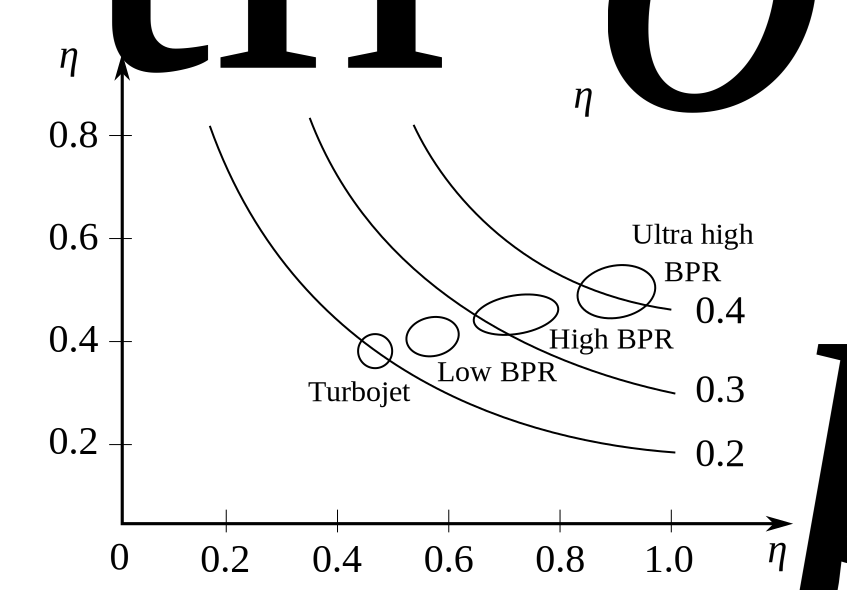
\includegraphics[width=0.54\textwidth]{etaThEtaP}
    \caption{\label{fig:ETA_OVERALL}Overall efficiency.}
  \end{center}
\end{figure}
%================================================================

%%%%%%%%%%%%%%%%%%%%%%%%%%%%%%%%%%%%%%%%%%%%%%%%%%%%%%%%%%%%%%%%%%
%\paragraph{Propeller Thrust}\mbox{} \\[0.5em]
%%%%%%%%%%%%%%%%%%%%%%%%%%%%%%%%%%%%%%%%%%%%%%%%%%%%%%%%%%%%%%%%%%
%Thrust generation by propeller is facilitated by imparting work to accelerate the fluid that passes through the propeller. Analysis of propeller performance follows classical turbomachinery analysis (see Sec. 7 of \cite{HILL_PETERSON_BOOK1992}; we will get back to this subject in our turbomachinery analysis to study compressor and turbine performance).
%
%To relate the propeller torque to the momentum difference across the propeller, we can conduct a kinematic analysis of the velocity field around a single propeller at a blade radius $r_B$. This analysis results in the so-called velocity-triangle. In this analysis, we differentiate between absolute (fixed coordinate systems) and relative (to blade) velocity:
%\begin{tabbing}
%  \qquad\= $U_\infty$: \= Fluid velocity, approach speed in fixed (absolute) coordinate systems;\\
%  \> $V_B$: \> Blade velocity, with $V_B = \Omega r_B$;\\
%  \> $W$: \> Fluid velocity, relative to rotating blade;\\
%  \> $\alpha$: \> absolute angle of attack;\\
%  \> $\beta$: \> blade angle.
%\end{tabbing}
%From the kinematic relation at the leading or trailing edge of the blade we can then construct the velocity triangle:
%\begin{equation}
% W + V_B = U_\infty \,.
%\end{equation}
%
%%================================================================
%\begin{figure}[!h!]
%  \begin{center}
%    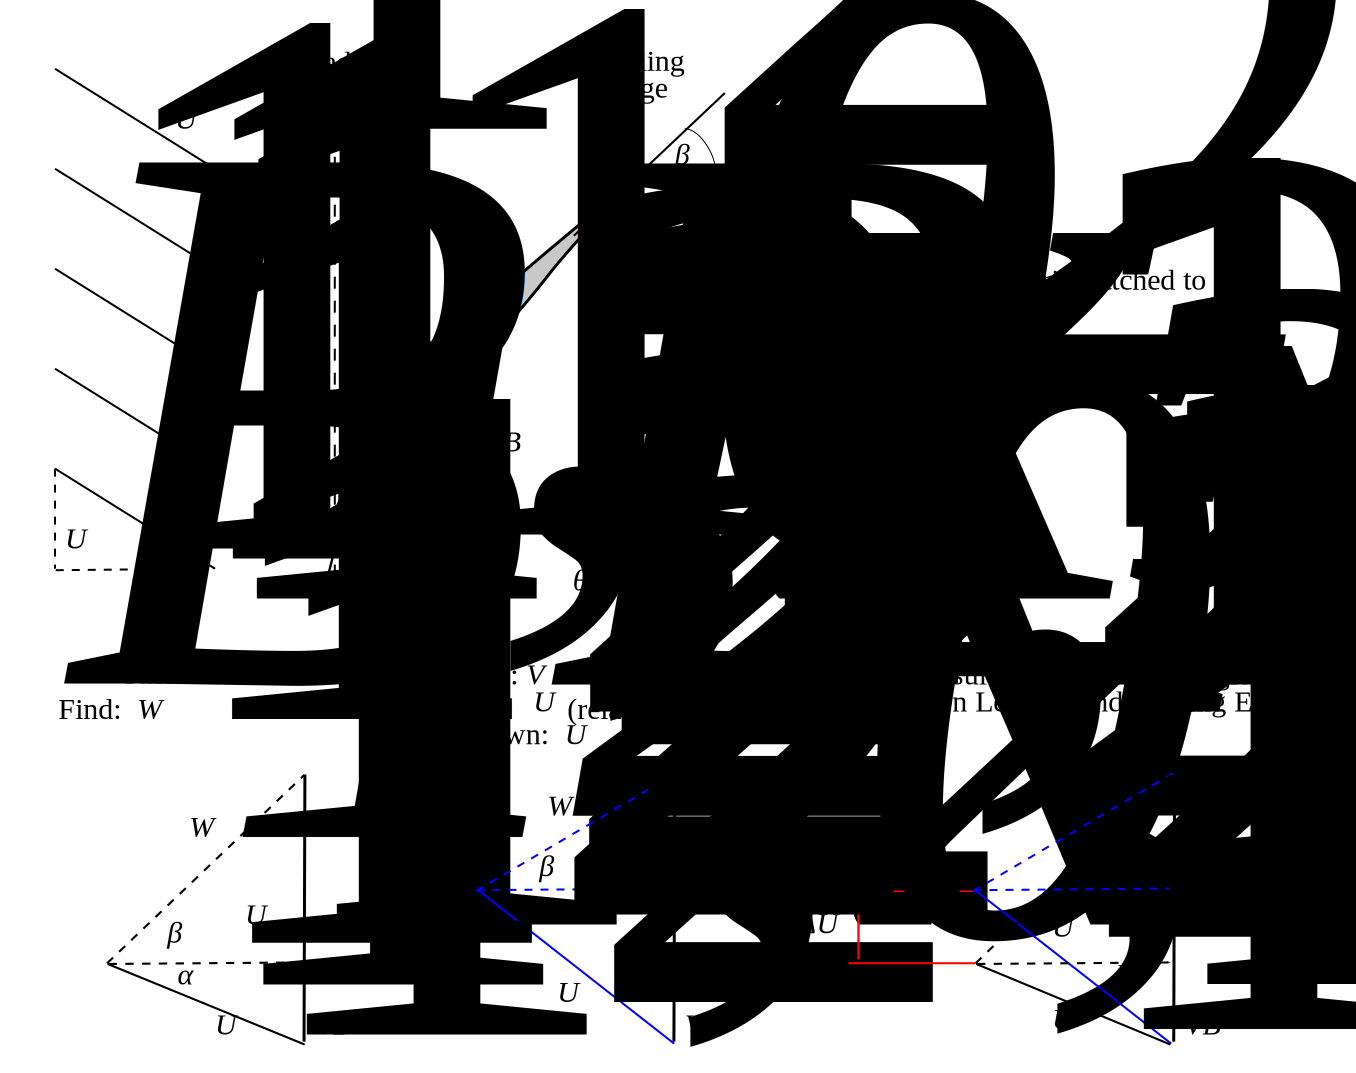
\includegraphics[width=0.95\textwidth]{velocityTriangle}
%  \caption{\label{FIG_VELOCITY_TRIANGLE}Velocity triangle.}
%  \end{center}
%\end{figure}
%%================================================================
%
%The construction of the velocity triangle at the leading and trailing edges of the propeller blade is illustrated in \cref{FIG_VELOCITY_TRIANGLE}. By superimposing both triangles, we can determine differences in azimuthal velocity components between trailing and leading edges:
%\begin{equation}
%  \Delta U_\theta = U_{\theta,2} - U_{\theta,1} \, \text{.}
%\end{equation}
%Similarly, we can also compute the axial velocity difference
%\begin{equation}
%  \Delta U_z = U_{z,2} - U_{z,1} \, \text{.}
%\end{equation}
%With this, we can evaluate the {\it torque} required to drive the propeller:
%\begin{equation}
%  \cT_{Prop}(r_B) = \dot{m}r_B\Delta U_{\theta} \, \text{,}
%\end{equation}
%or by considering a control area, we can evaluate the entire torque of the propeller
%\begin{equation}
%  \cT_{Prop} = N_{B} \int^R_0 2\pi \rho U_{\infty,z}r^2(\Delta U_\theta)dr \, \text{,}
%\end{equation}
%where $N_B$ is the number of blades.
%
%The propeller power is then evaluated as:
%\begin{equation}
%  \cP_{Prop} = \cT_{Prop}\Omega \, \text{,}
%\end{equation}
%where  $\Omega$ is the angular speed of the propeller (in units of s$^{-1}$). By accounting for the efficiency of the propeller in converting mechanical into technical work, we introduce a propeller efficiency $\eta_{Prop}$:
%\begin{equation}
%  \cP_{Prop} = {\eta_{Prop}}\cP_{Engine} \, \text{,}
%\end{equation}
%where $\cP_{Engine}$ is the required engine power. 
%
%With the thrust equation (derived in the next section) we can relate the axial velocity difference across the propeller to the thrust:
%\begin{equation}
% T = \dot{m}\Delta U_z \, \text{.}
%\end{equation}
%Note that we can typically neglect any area contraction or ram-effects upstream of the propeller, so that $U_\infty$ remains constant.
%
%%%%%%%%%%%%%%%%%%%%%%%%%%%%%%%%%%%%%%%%%%%%%%%%%%%%%%%%%%%%%%%%%%
%\paragraph{Propulsive Efficiency}\mbox{} \\[0.5em]
%%%%%%%%%%%%%%%%%%%%%%%%%%%%%%%%%%%%%%%%%%%%%%%%%%%%%%%%%%%%%%%%%%
%The {\it overall efficiency} is defined as:
%\begin{eqnarray}
%  \eta_O&=&\f{\text{Propulsive Power}}{\text{Total Power/Energy Available in Fuel}}\\
%        &=& \underbrace{\f{\text{Propulsive Power}}{\text{Flow Power}}}_{\text{Propulsive Efficiency $\eta_P$}}
%            \underbrace{\f{\text{Flow Power}}{\text{Total Power/Energy Available in Fuel}}}_{\text{Thermal Efficiency $\eta_{th}$}}
%\end{eqnarray}
%and with the definitions:
%\begin{tabbing}
%  \qquad\= Propulsive Power:\quad\= $P_P$\= $=TU_\infty$, \\
%  \> Flow Power: \> $P_F$\> $=KE_{out}-KE_{in}$\\[1mm]
%  \> \>\> $=\f{1}{2}\dot{m}_eU^2_e-\f{1}{2}\dot{m}_iU^2_\infty$\\[1mm]
%  \> \>\> $=\f{1}{2}\dot{m}_i\left[(1+f)U^2_e-U^2_\infty\right]$.
%\end{tabbing}
%
%The {\it propulsive efficiency} is defined as:
%\begin{eqnarray}
%  \eta_P&=&\f{TU_\infty}{\f{1}{2}\dot{m}_i[(1+f)U^2_e-U^2_\infty]} \, \text{,}
%\end{eqnarray}
%with \cref{EQ_THRUST_EQUATION} for the expression for thrust, and the thermal efficiency is specific to the thermodynamic cycle. After introducing the simplifications $f\ll1$ (with $f=\f{\dot{m}_f}{\dot{m}_{air}}$ being the fuel/air ratio) and pressure thrust $\ll$ jet thrust, we have
%\begin{equation}
%  \eta_P=\f{2}{\left(\f{U_e}{U_\infty}+1\right)}
%\end{equation}
%so that $0\le\eta_P\le2$. Maximizing $\eta_P$ requires $U_e\to 0.$ However, to maximize thrust we requires $U_e\to \infty$. \Cref{FIG_CV_ANALYSIS_THRUST_EQUATION} shows the variation of propulsive efficiency and thrust against velocity ratio.
%
%%================================================================
%\begin{figure}[t!]
%  \begin{center}
%    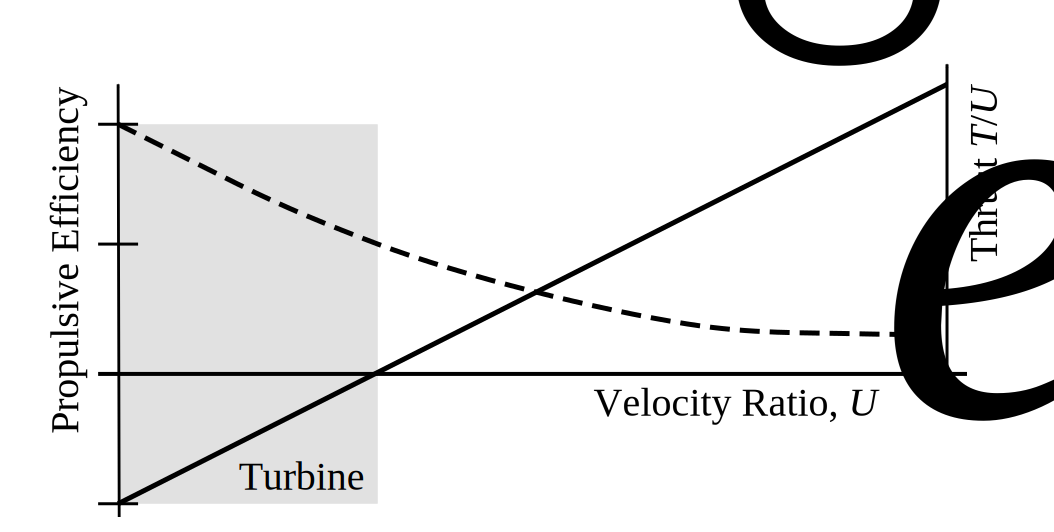
\includegraphics[width=0.6\textwidth]{efficiencyThrustCurve}
%    \caption{\label{FIG_CV_ANALYSIS_THRUST_EQUATION}Propulsive efficiency and thrust vs. velocity ratio.}
%  \end{center}
%\end{figure}
%%================================================================
%\vspace*{1in}

\clearpage
%%%%%%%%%%%%%%%%%%%%%%%%%%%%%%%%%%%%%%%%%%%%%%%%%%%%%%%%%%%%%%%%%
\section{Altitude Effects}
%%%%%%%%%%%%%%%%%%%%%%%%%%%%%%%%%%%%%%%%%%%%%%%%%%%%%%%%%%%%%%%%%

The thermodynamic state of the atmosphere changes with altitude, thereby affecting the aircraft performance (thrust and lift, etc). 

The temperature in the atmosphere follows a complicated function (see \cref{FIG_ALTITUDE}), in which different physical processes become important (such as buoyancy and radiation, etc) in controlling the ambient state at different altitude. 

%================================================================
\begin{figure}[!h!]
  \begin{center}
    \includegraphics[width = 0.95\textwidth]{atmosphere}
  \end{center}
  \caption{\label{FIG_ALTITUDE}Earth atmosphere (source: \url{www.theozonehole.com}).}
\end{figure}
%================================================================

Since the flight altitude of airbreathing vehicles is limited by constraints on the required lift (density), available oxygen concentration, and environmental impact and emissions, we restrict our analysis to the troposphere ($h\le 12$ km). To good accuracy, this layer can be characterized by an isotropic process, and from a force balance between buoyancy and pressure forces acting on a differential control volume, we can derive the following altitude-dependent state relation for temperature $T(z)$, density $\rho(z)$, and pressure $p(z)$:
\begin{subeqnarray}
  \f{T(z)}{T_s} &=& \left[1-\f{\gamma-1}{\gamma}\left(\f{z}{\wt{z}}\right)\right]\\
  \f{\rho(z)}{\rho_s} &=& \left[1-\f{\gamma-1}{\gamma}
                          \left(\f{z}{\wt{z}}\right)\right]^{\f{1}{\gamma-1}}\\
  \f{p(z)}{p_s} &=& \left[1-\f{\gamma-1}{\gamma}\left(\f{z}{\wt{z}}\right)\right]^{\f{\gamma}{\gamma-1}}
\end{subeqnarray}
where
\begin{equation}
  \wt{z} = \f{p_s}{\rho_s g}\, \text{,}
\end{equation}
and $p_s=101$,325 Pa, $\rho_s=1.23$ kg/m$^3$, and $T_s=288$ K.

A comparison of the isentropic model with the International Standard Atmosphere (ISA) is shown in Fig.~\ref{FIG_ISAISENCOMPARE}. The ISA model is created by presuming a temperature profile (piece-wise linear for the altitudes shown), and computing the pressure and density from the hydrostatic pressure distribution and ideal gas law. That is,

\begin{equation}
	\begin{aligned}
		\frac{\d p}{\d z}&=-\rho g\ , \\
		\rho &= \frac{p}{RT(z)}.
	\end{aligned}
\end{equation}
Combining and integrating, one obtains
\begin{equation}
	\begin{aligned}
		\frac{p(\hat z)}{p_\mathrm{s}}=\exp\left(-\int_0^{\hat z} \frac{T_\mathrm{s}}{T(\hat z')}\d \hat z'\right)\ ,
	\end{aligned}
\end{equation}
where $\hat z=z/\tilde z$ is used for brevity.

As shown in the figure, the two models follow rather closely for the density and pressure but not the temperature. MATLAB contains the function "atmosisa", which gives the ISA model's thermodynamic conditions as a function of altitude. It is recommended that this function be used in the homework .

%================================================================
\begin{figure}[!h!]
	\begin{center}
		\includegraphics[width = 0.95\textwidth]{atmosphericPropertiesComparison.pdf}
	\end{center}
	\caption{\label{FIG_ISAISENCOMPARE} The ISA model (--) compared against the isentropic model (- -).}
\end{figure}
%================================================================\clearpage
%%%%%%%%%%%%%%%%%%%%%%%%%%%%%%%%%%%%%%%%%%%%%%%%%%%%%%%%%%%%%%%%%
\section{Thermodynamics}
%%%%%%%%%%%%%%%%%%%%%%%%%%%%%%%%%%%%%%%%%%%%%%%%%%%%%%%%%%%%%%%%%
In the previous sections, we already used basic concepts of gas dynamics to derive the thrust equation. Here, we review all essential gas-dynamic and thermodynamic concepts that we need for the gas turbine cycle analysis.
%%%%%%%%%%%%%%%%%%%%%%%%%%%%%%%%%%%%%%%%%%%%%%%%%%%%%%%%%%%%%%%%%
\subsection{Conservation Equations}
%%%%%%%%%%%%%%%%%%%%%%%%%%%%%%%%%%%%%%%%%%%%%%%%%%%%%%%%%%%%%%%%%
Recall the general form of a conservation equation of any quantity $\phi = \{{\text{mass},\, \text{momentum},\, \text{energy}}$\},
\begin{equation}
\text{accumulation}(\phi) + \text{outflow}(\phi) - \text{inflow}(\phi) = \text{production}(\phi)\,.
\end{equation}
For the following analysis, we will consider a control volume analysis, which is illustrated in \cref{FIG_CONTROL_VOLUME}.

%================================================================
\begin{figure}[!hbt!]
  \begin{center}
    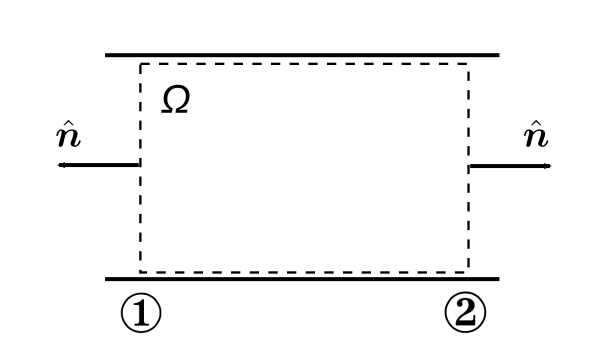
\includegraphics[width=0.38\textwidth]{ControlVolume}
    \caption{\label{FIG_CONTROL_VOLUME}Control volume.}
  \end{center}
\end{figure}
%================================================================

%%%%%%%%%%%%%%%%%%%%%%%%%%%%%%%%%%%%%%%%%%%%%%%%%%%%%%%%%%%%%%%%%
\subsubsection{Mass Conservation}
%%%%%%%%%%%%%%%%%%%%%%%%%%%%%%%%%%%%%%%%%%%%%%%%%%%%%%%%%%%%%%%%%
The governing equation describing conservation of mass can be written in the following form:
\begin{equation}
  \f{dm}{dt} = \dot{m}_\text{in} - \dot{m}_\text{out} = - \oint \rho \uvec \cdot \hat{\nvec} dA\,,
\end{equation}
where $\dot{m} = \int \rho u_\perp dA$, in which $u_\perp$ is the velocity component normal to the area $A$. For stationary flows, $dm/dt = 0$, and hence we have $\dot{m}_\text{in} = \dot{m}_\text{out}$, or
\begin{equation}
  \rho_1 u_{\perp1} A_1 = \rho_2 u_{\perp2} A_2\,,
\end{equation}
which is called the one-dimensional mass-flow equation.

%%%%%%%%%%%%%%%%%%%%%%%%%%%%%%%%%%%%%%%%%%%%%%%%%%%%%%%%%%%%%%%%%
\subsubsection{Momentum Conservation}
%%%%%%%%%%%%%%%%%%%%%%%%%%%%%%%%%%%%%%%%%%%%%%%%%%%%%%%%%%%%%%%%%
The governing equation describing conservation of momentum conservation takes the following form:
\begin{equation}
  \begin{split}
    \f{d(m \uvec)}{dt} = \f{d}{dt} \int \rho\uvec dV &= \dot{M}_\text{in} - \dot{M}_\text{out} + \sum_i \Fvec_i \\
                         &= - \oint (\rho \uvec)( \uvec \cdot \hat{\nvec}) dA + \sum_i \Fvec_i\,,
  \end{split}
\end{equation}
which is a vector equation for each velocity component $\uvec=(u_1, u_2,\ldots)^T\in\mathbb{R}^{N_d}$ (with $N_d$ being the spatial dimension). The force terms on the right-hand side are:
\begin{itemizePacked}
  \item Pressure force: $\Fvec_p = -\int \nabla p dV$;
  \item Viscous force: $\Fvec_v = -\oint \hat{\nvec} \cdot \sigmamat dA$;
  \item Gravitational force: $\Fvec_g = \int \rho \gvec dV$.
%  \item Reaction force: $\Fvec_p = -\int \nabla p dV$.
\end{itemizePacked}
Under the assumption of steady-state, the momentum conservation equation reduces to:
\begin{equation}
  \dot{M}_\text{in} - \dot{M}_\text{out}  = -\sum_i \Fvec_i\,,
\end{equation}
or for one-dimensional flows:
\begin{equation}
  (\rho_2 u_{\perp2} A_2)u_{\perp2}-(\rho_1 u_{\perp1} A_1)u_{\perp1} = p_1A_1-p_2A_2-F_D\,,
\end{equation}
where $F_D$ is the drag force, as shown in \cref{FIG_MOMENTUM_CONSERVATION}.

%================================================================
\begin{figure}[!h!]
  \begin{center}
    \includegraphics[width=0.65\textwidth]{MomentumConservation}
    \caption{\label{FIG_MOMENTUM_CONSERVATION}Momentum balance on control volume.}
  \end{center}
\end{figure}
%================================================================

%%%%%%%%%%%%%%%%%%%%%%%%%%%%%%%%%%%%%%%%%%%%%%%%%%%%%%%%%%%%%%%%%
\subsubsection{Energy Conservation}
%%%%%%%%%%%%%%%%%%%%%%%%%%%%%%%%%%%%%%%%%%%%%%%%%%%%%%%%%%%%%%%%%
We define the total energy as $H_T = H + \f{1}{2}m\uvec^2+mgz$ or in mass-specific form
\begin{equation}
h_T = h + \f{1}{2} u^2 + gz = h_0 + gz\,.
\end{equation}
The conservation equation is
\begin{equation}
  \f{d}{dt} \int \rho h_T dV + \oint \rho h_T (\uvec \cdot \hat{\nvec})dA =  \underbrace{\int \dot{Q} dV}_\text{Heat transfer rate}+\underbrace{\f{d}{dt}\int p dV}_\text{Technical work}+\underbrace{\int F_\sigma dV}_\text{Viscous force}\,,
\end{equation}
where $\dot{q}$ is the heat transfer rate (per unit time and unit volume). Using Fourier's law, $\dot{q}$ can be written as $\dot{q} = \nabla \cdot (\lambda \nabla T)$), and $F_\sigma = \nabla \cdot (\sigmamat \cdot \uvec)$ is the viscous dissipation.

%================================================================
\begin{figure}[!h!]
  \begin{center}
    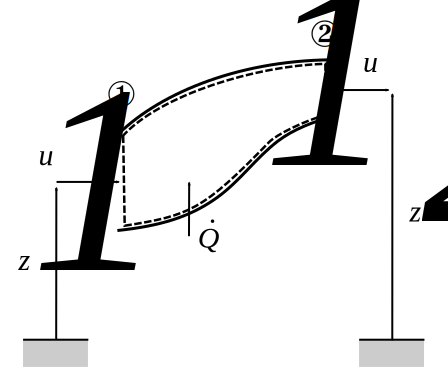
\includegraphics[width=0.52\textwidth]{EnergyConservation}
    \caption{\label{FIG_ENERGY_CONSERVATION}Control volume balance for energy equation.}
  \end{center}
\end{figure}
%================================================================

%%%%%%%%%%%%%%%%%%%%%%%%%%%%%%%%%%%%%%%%%%%%%%%%%%%%%%%%%%%%%%%%%
\subsubsection{Summary of Governing Equations}
%%%%%%%%%%%%%%%%%%%%%%%%%%%%%%%%%%%%%%%%%%%%%%%%%%%%%%%%%%%%%%%%%
In the following, we summarize the set of working equations in differential form that we will use for the subsequent analysis:
\begin{itemizePacked}
  \item Mass conservation: 
    \begin{equation}
      \partial_t \rho + \nabla \cdot (\rho \uvec) = 0\,;
    \end{equation}
  \item Momentum conservation: 
    \begin{equation}
      \partial_t (\rho \uvec) + \nabla \cdot (\rho \uvec \otimes \uvec) = - \nabla p + \nabla \cdot \sigmamat\,;
    \end{equation}
  \item Energy conservation: 
    \begin{equation}
      \partial_t (\rho h_T) + \nabla \cdot (\rho \uvec h_T) = \partial_t p + \nabla \cdot \dot{\qvec} + \nabla \cdot (\sigmamat \cdot \uvec)\,,
    \end{equation}
\end{itemizePacked}
where
\begin{equation}
\sigmamat = \mu(\nabla \uvec + (\nabla \uvec)^T) - \frac{2}{3} \mu (\nabla \cdot \uvec) \Imat\,.
\end{equation}

%%%%%%%%%%%%%%%%%%%%%%%%%%%%%%%%%%%%%%%%%%%%%%%%%%%%%%%%%%%%%%%%%
\subsection{Thermodynamics of Gases}
%%%%%%%%%%%%%%%%%%%%%%%%%%%%%%%%%%%%%%%%%%%%%%%%%%%%%%%%%%%%%%%%%

%%%%%%%%%%%%%%%%%%%%%%%%%%%%%%%%%%%%%%%%%%%%%%%%%%%%%%%%%%%%%%%%%
\subsubsection{First Law of Thermodynamics}
%%%%%%%%%%%%%%%%%%%%%%%%%%%%%%%%%%%%%%%%%%%%%%%%%%%%%%%%%%%%%%%%%
For a closed system (control volume), the first law of thermodynamics takes the following form:
\begin{equation}
  d e = \delta q - \delta w_m\;,
\end{equation}
where the mechanical work (moving-boundary work) is written as $\quad \delta w_m = pdv$. The corresponding energy equation for an open thermodynamic system is;
\begin{equation}
  d h = \delta q - \delta w_t\;,
\end{equation}
where the technical work (compressor/turbine work) is  $\delta w_t =-vdp = 
\f{1}{\rho}dp$.

%%%%%%%%%%%%%%%%%%%%%%%%%%%%%%%%%%%%%%%%%%%%%%%%%%%%%%%%%%%%%%%%%
\subsubsection{Second Law of Thermodynamics}
%%%%%%%%%%%%%%%%%%%%%%%%%%%%%%%%%%%%%%%%%%%%%%%%%%%%%%%%%%%%%%%%%
The second law of thermodynamics provides a relation about the directionality of a thermodynamic process, by introducing entropy as a measure for the reversibility of a thermodynamic process. In general, entropy is a measure for information content, and, in the context of thermodynamics, we associate entropy as direct link between micro- and macro-states. This link can be established through statistical thermodynamics. 

The change in entropy provides information about a reversible process. Consider states (1) and (2): if $dS = S_2 - S1=0$ then the process is reversible. For a system that is not in equilibrium, $d S \ge 0$. To quantify irreversible contributions, we extend the second law by formally introducing an irreversible contribution $\Delta S_{\rm{irr}}$. With this, we can write the second law in a general form as:
\begin{equation}
  dS = \f{\delta Q}{T} + \Delta S_{\rm{irr}}\ge 0 \, \text{.}
\end{equation}
Typical sources of irreversibilities are:
\begin{itemizePacked}
 \item Shocks
 \item Combustion
 \item Friction
 \item Separation
 \item Mixing
 \item Phase transition
\end{itemizePacked}
For practical applications, irreversibilities reduce the thermodynamic efficiency since heat and work is required to overcome $\Delta S_{\rm{irr}}$.
%%%%%%%%%%%%%%%%%%%%%%%%%%%%%%%%%%%%%%%%%%%%%%%%%%%%%%%%%%%%%%%%%
\subsubsection{Equation of State}
%%%%%%%%%%%%%%%%%%%%%%%%%%%%%%%%%%%%%%%%%%%%%%%%%%%%%%%%%%%%%%%%%
From gas dynamic theory, we are able to relate the macroscopic pressure to the mean particle speed $\ol{c}$ (see \cite{VINCENTI_KRUGER_BOOK1965}):
\begin{equation}
  p = \f{1}{3}\rho\ol{c}^2 \, \text{.}
\end{equation}
Since $\ol{c}$ is a function of temperature, we can directly relate pressure to temperature and density:
\begin{equation}
  \label{EQ_STATE_RELATION}
  p = f(\rho,T)\;,
\end{equation}
providing a formal description for a general state-relation. A specific form of the state-equation (\ref{EQ_STATE_RELATION}) is the {\it ideal gas law}:
\begin{equation}
  p = \rho R  T
\end{equation}
where the gas constant $R$ is introduced as proportionality constant. We can express the ideal gas law in the following different, but equivalent, forms:
\begin{itemizePacked}
  \item {\it Mole-specific} quantities:
  \[
   p V=  n \cR T \, \text{;}
  \]
  \item {\it Mass-specific} quantities:
  \[
   p V= m R T \qquad \Leftrightarrow\qquad p = \rho R T \, \text{;}
  \]
  \item {\it Particle-specific} quantities:
  \[
   p V= N k_B T
  \]
  with $k_B = \cR/N_A$ and $N_An=N.$
\end{itemizePacked}
The ideal gas law (IGL) is only one but rather powerful example of a state-equation. In general, we define a {\it state equation} as a constitutive relation between two or more thermodynamic variables. 

The IGL is very accurate as long as the intermolecular spacing between particles is sufficiently large (``Knudsen limit''). However, when the pressure $p$ gets large enough and/or the temperature is low (cryogenic) the intermolecular forces become increasingly important, and the IGL becomes invalid. Such high-pressure conditions require the consideration of so-called real-fluid effects, and can be accommodated by extending the state relation in the following form:
\begin{equation}
  p = Z \rho R T
\end{equation}
where $Z$ is the compressibility factor, with
\begin{eqnarray}
  Z &=&\left\{ 
         \begin{array}{r@{:\quad}l}
          = 1& {\text{for ideal gas}}\\
          \ne 1& {\text{real fluid and extension to super/sub-critical fluid mixtures}}
         \end{array}
         \right. \, \text{.}
\end{eqnarray}

Real fluid effects are often described by {\it cubic state equations}. The general form of a cubic state relation can be written in the form: 
\begin{equation}
  p = \f{\cR T}{V_m -b}- \f{\Theta (V_m-\eta)}{(V_m-b)(V^2_m+\delta V + \eps)}
\end{equation}
where $V_m = M/\rho = V/n$ is the molar volume, and the parameters $\Theta, b, \eta, \eps, \delta$ depend on temperature, mixture and critical conditions. Examples of commonly employed cubic state relations are equations due to
\begin{itemizePacked} 
  \item Peng-Robinson (PR);
  \item Redlich-Kwong (RK);
  \item Soave-Redlich-Kwong (SRK).
\end{itemizePacked}

The consideration of real fluid effects is relevant if either pressure or temperature of the gas exceeds the critical point (see \cref{FIG_PHASE_DIAGRAM}). Relevant applications are  rocket-engines and combustion in high-pressure aviation gas-turbines in which  the combustion chamber pressure exceeds the critical pressure. Values for critical pressure and temperature conditions that are relevant for our lecture are summarized in \cref{TAB_CRITICAL_CONDITIONS}.
 
%================================================================
\begin{figure}[!h!]
  \begin{center}
    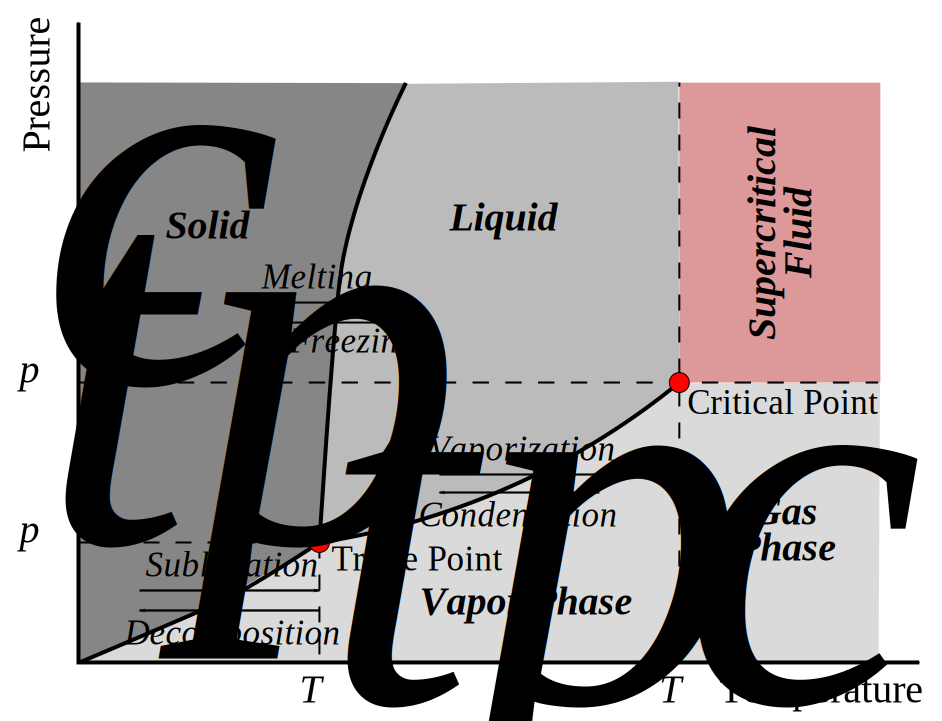
\includegraphics[width=0.58\textwidth]{phaseDiagram}
    \caption{\label{FIG_PHASE_DIAGRAM}Phase diagram.}
  \end{center}
\end{figure}
%================================================================

 %===============================================================
\begin{table}[!h!]
\begin{center}
\begin{tabular}{|c|cc|}\hline
&$T_c$ [K]& $p_c$ [bar]\\\hline\hline
\chem{H_2} & 33.2 & 13.0\\
\chem{O_2} & 154.6 & 50.5 \\
\chem{N_2} & 126.3 & 33.9\\
\chem{CH_4}& 190.9 & 46.4\\\hline
\end{tabular}
\caption{\label{TAB_CRITICAL_CONDITIONS}Critical conditions for selected gases.}
\end{center}
\end{table}
%===============================================================

%%%%%%%%%%%%%%%%%%%%%%%%%%%%%%%%%%%%%%%%%%%%%%%%%%%%%%%%%%%%%%%%%
\subsubsection{Constitutive Relations}
%%%%%%%%%%%%%%%%%%%%%%%%%%%%%%%%%%%%%%%%%%%%%%%%%%%%%%%%%%%%%%%%%
For a thermally perfect  gas, the sensible internal energy and enthalpy are only dependent on temperature:
\begin{equation}
 e = e(T) \quad \text{and} \quad h = h(T)\,.
\end{equation}
The {\it specific heat capacities} are defined as
\begin{equation}
  c_p = \left.\f{dh}{dT}\right|_p \quad \text{and} \quad c_v = \left.\f{de}{dT}\right|_v\,.
\end{equation}
The {\it ratio of specific heat capacities} is then defined as
\begin{equation}
 \gamma = \f{c_p}{c_v}\quad\text{and}\quad R = c_p - c_v \, \text{.}
\end{equation}

Remarks:
\begin{itemizePacked}
 \item For our thermodynamic analysis, we frequently make use of the calorically perfect gas assumption, stating that $c_p$ and $c_v$ are constant and independent of temperature.
 This reduces the mathematical complexity, since it allows to directly evaluate enthalpy and internal energy in terms of algebraic relations of temperature.
 \item In general, the specific heat capacities of a gas mixture are dependent on species composition and temperature
 \begin{equation}
  c_p = c_p(\Yvec,T)\qquad\text{with}\qquad c_p = \sum_{i=1}^{N_s} Y_i c_{p,i}\;.
 \end{equation}
 \item For practical applications, the species-specific heat capacities at constant pressure are commonly tabulated in terms of higher-order 
 polynomial expressions:
 \[
  \f{c_{p}}{R} = \sum^4_{i=-2} a_i T^i \, \text{.}
 \]
Coefficients of these polynomials are tabulated in the form of NASA polynomial tables~\cite{MCBRIDE_ZEHE_GORDON_NASA2002}.
\end{itemizePacked}
%%%%%%%%%%%%%%%%%%%%%%%%%%%%%%%%%%%%%%%%%%%%%%%%%%%%%%%%%%%%%%%%%
\subsubsection{Isentropic Relation}
%%%%%%%%%%%%%%%%%%%%%%%%%%%%%%%%%%%%%%%%%%%%%%%%%%%%%%%%%%%%%%%%%
The entropy relation takes the following form
\begin{equation}
  ds = \f{dh}{T} - \f{dp}{\rho T}
\end{equation}
for a reversible process and with $dh = c_p dT$, $c_p = \f{\gamma}{\gamma-1}R$, and $\rho T = p/R$, we have two other forms of the entropy relation:
\begin{equation}
  ds = \f{\gamma}{\gamma-1}R \f{dT}{T} - R \f{dp}{p}\,,
\end{equation}
and
\begin{equation}
  ds = \f{1}{\gamma-1}R \f{dT}{T} - R \f{d\rho}{\rho}\,.
\end{equation}
These equations are commonly referred to as Gibbs' equations or as Gibbs-Duhem equation for multicomponent mixtures.

The speed of sound is defined by:
\begin{equation}\label{a2}
  a^2 \equiv \left( \frac{\partial p}{\partial \rho} \right)_s \, \text{,}
\end{equation}
where the subscript `s' indicates that the partial derivative is evaluated at constant entropy. It is useful to write \cref{a2} as the sum of constant energy and constant density processes, giving:
\begin{equation}
a^2 = \left(\frac{\partial p}{\partial \rho} \right)_e +
\frac{p}{\rho^2} \left(\frac{\partial \rho}{\partial e}
\right)_\rho \, \text{.}
\end{equation}
By introducing the calorically-perfect gas approximation, and rewriting the internal energy as:
\begin{equation}
e = c_v T = \frac{1}{\gamma-1}RT = \frac{1}{(\gamma -
1)}\frac{p}{\rho}\qquad\Rightarrow\qquad
p = (\gamma -1) \rho e \,
\end{equation}
%using the equation of state in the form of Eq. (\ref{EOS2}),
%which states $p=(\gamma-1)\rho e$, 
(setting the reference condition to zero). We can write the following useful expressions for the speed of sound:
\begin{equation}
  \begin{split}
a^2 &= (\gamma-1)e + \frac{p}{\rho^2}(\gamma-1)\rho  \\
&=(\gamma-1) \left(e + \frac{p}{\rho} \right) \\
&= (\gamma - 1)h\\
&= (\gamma-1)c_p T  \\
&= \gamma R T  \\
&= \frac{\gamma p}{\rho} \, \text{.}
  \end{split}
\end{equation}

%%%%%%%%%%%%%%%%%%%%%%%%%%%%%%%%%%%%%%%%%%%%%%%%%%%%%%%%%%%%%%%%%
\subsubsection{Stagnation Conditions}
%%%%%%%%%%%%%%%%%%%%%%%%%%%%%%%%%%%%%%%%%%%%%%%%%%%%%%%%%%%%%%%%%
For gas turbine analysis, it is convenient to perform the analysis in terms of stagnation conditions. For this, we define the total enthalpy (or stagnation enthalpy) as:
\begin{equation}
 \label{EQ_stagnation_ENTH}
  h_0 = h + \f{1}{2} u^2 \,.
\end{equation}
combining sensible enthalpy and mass-specific kinetic energy. For a calorically perfect gas, we write:
\begin{equation}
  h = c_p (T-T_\text{ref})\,,
\end{equation}
so that \cref{EQ_stagnation_ENTH} can be written as:
\begin{equation}
T_0 = T + \frac{u^2}{2c_p}\;,
\end{equation}
with $c_p = \f{\gamma}{\gamma-1}R$, $\gamma R T = a^2$ and the Mach number as $\text{M} = {u}/{a}$, it follows:
\begin{equation}
  \f{T_0}{T} = 1+ \left(\f{\gamma-1}{2}\right) \text{M}^2\;.
\end{equation}
With isentropic state relations: 
\begin{equation}
  \f{p_0}{p} = \left(\f{T_0}{T}\right)^\f{\gamma}{\gamma-1} \quad \text{and} \quad \f{\rho_0}{\rho} = \left(\f{p_0}{p}\right)^\f{1}{\gamma}\,,
\end{equation}
we obtain relation for stagnation pressure and stagnation temperature:
\begin{eqnarray}
  \f{p_0}{p} &=& \left[1+ \left(\f{\gamma-1}{2}\right) \text{M}^2\right]^\f{\gamma}{\gamma-1}\,,\\
  \f{\rho_0}{\rho} &=& \left[1+ \left(\f{\gamma-1}{2}\right) \text{M}^2\right]^\f{1}{\gamma-1}\,.
\end{eqnarray}

%===============================================================
\setboolean{@twoside}{false}
\includepdf[pages=-,scale=0.82,offset=75 -75,pagecommand={},angle=180]{handout06TDProcesses.pdf}
%===============================================================



\clearpage
%%%%%%%%%%%%%%%%%%%%%%%%%%%%%%%%%%%%%%%%%%%%%%%%%%%%%%%%%%%%%%
\section{Aircraft Jet Engines}
%%%%%%%%%%%%%%%%%%%%%%%%%%%%%%%%%%%%%%%%%%%%%%%%%%%%%%%%%%%%%%

%%%%%%%%%%%%%%%%%%%%%%%%%%%%%%%%%%%%%%%%%%%%%%%%%%%%%%%%%%%%%%
\subsection{General Gas Turbine Engine Concepts}
%%%%%%%%%%%%%%%%%%%%%%%%%%%%%%%%%%%%%%%%%%%%%%%%%%%%%%%%%%%%%%

%%%%%%%%%%%%%%%%%%%%%%%%%%%%%%%%%%%%%%%%%%%%%%%%%%%%%%%%%%%%%%
\subsubsection{Engine Design}
%%%%%%%%%%%%%%%%%%%%%%%%%%%%%%%%%%%%%%%%%%%%%%%%%%%%%%%%%%%%%%
\Cref{FIG_TSFC_MACH} shows functional relations between TFSC and Mach number for different types of jet engines. The objective of the engine design is to maximize the thrust. Since $T \sim \dot{m}_A(U_e - U_0)$, this is similar to maximizing the air flow rate and $U_0$. This is best accomplished with continuous flow engines, compared to cyclic engine concepts, such as IC/reciprocating engines.

At low-speed conditions, propellers are best suited to handle the airflows and piston engines are more efficient at low power setting. However, propellers become inefficient $\M > 0.5.$ Reason for this is that propeller-tip speed becomes supersonic, which results in substantial losses and noise generation. 

%==============================================================
\begin{figure}[!htb!]
 \centering
    {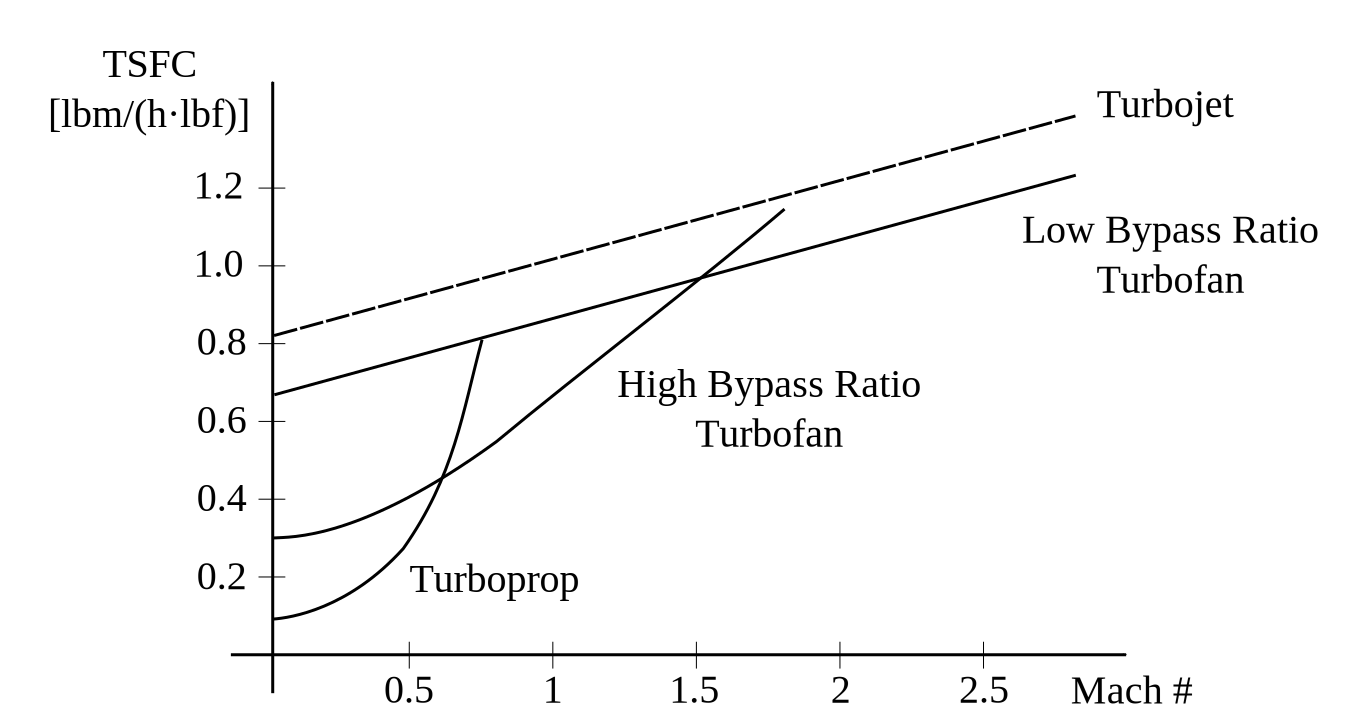
\includegraphics[width=0.85\textwidth, clip=, keepaspectratio]{TSFCMachRelation}}
    \caption{\label{FIG_TSFC_MACH}Relation between TSFC and Mach number for different jet engines.}
\end{figure}
%==============================================================

%%%%%%%%%%%%%%%%%%%%%%%%%%%%%%%%%%%%%%%%%%%%%%%%%%%%%%%%%%%%%%
\subsubsection{Categories of Gas Turbine Engines}
%%%%%%%%%%%%%%%%%%%%%%%%%%%%%%%%%%%%%%%%%%%%%%%%%%%%%%%%%%%%%%
In the following, we provide graphic illustrations of relevant gas-turbine engine concepts.
\begin{itemizePacked}
\item Basic gas generator (\cref{FIG_BASIC_GAS_GENERATOR})

%==============================================================
\begin{figure}[!h!]
 \centering
    {\includegraphics[width=0.74\textwidth, clip=, keepaspectratio]{basicGasGenerator}}
    \caption{\label{FIG_BASIC_GAS_GENERATOR}Basic gas generator.}
\end{figure}
%==============================================================

\item Turbojet (\cref{FIG_TURBOJET})

%==============================================================
\begin{figure}[!htb!]
 \centering
    {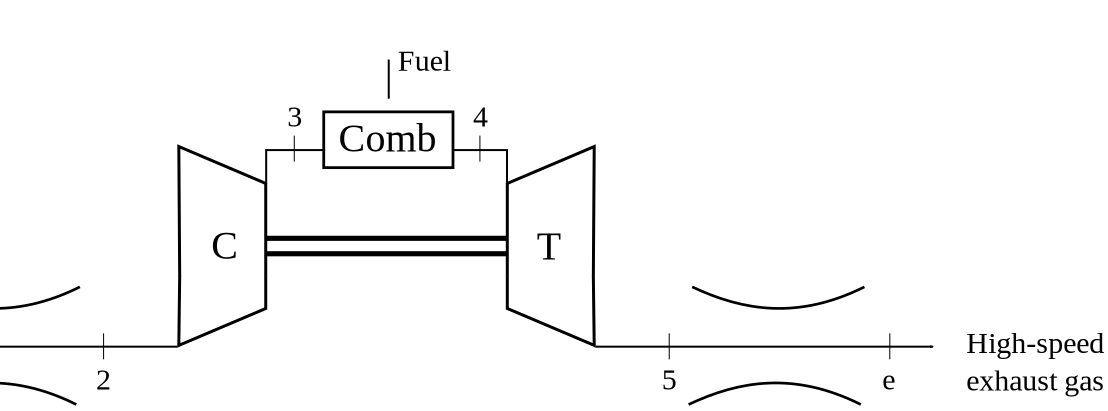
\includegraphics[width=0.88\textwidth, clip=, keepaspectratio]{turbojet}}
    \caption{\label{FIG_TURBOJET}Turbojet engine.}
\end{figure}
%==============================================================

\item Turbofan (\cref{FIG_TURBOFAN})

%==============================================================
\begin{figure}[!htb!]
 \centering
    {\includegraphics[width=0.95\textwidth, clip=, keepaspectratio]{turbofan}}
    \caption{\label{FIG_TURBOFAN}Turbofan engine.}
\end{figure}
%==============================================================

\item Multi-spool turbofan (\cref{FIG_MULTI_TURBOFAN})

%==============================================================
\begin{figure}[!htb!]
 \centering
    {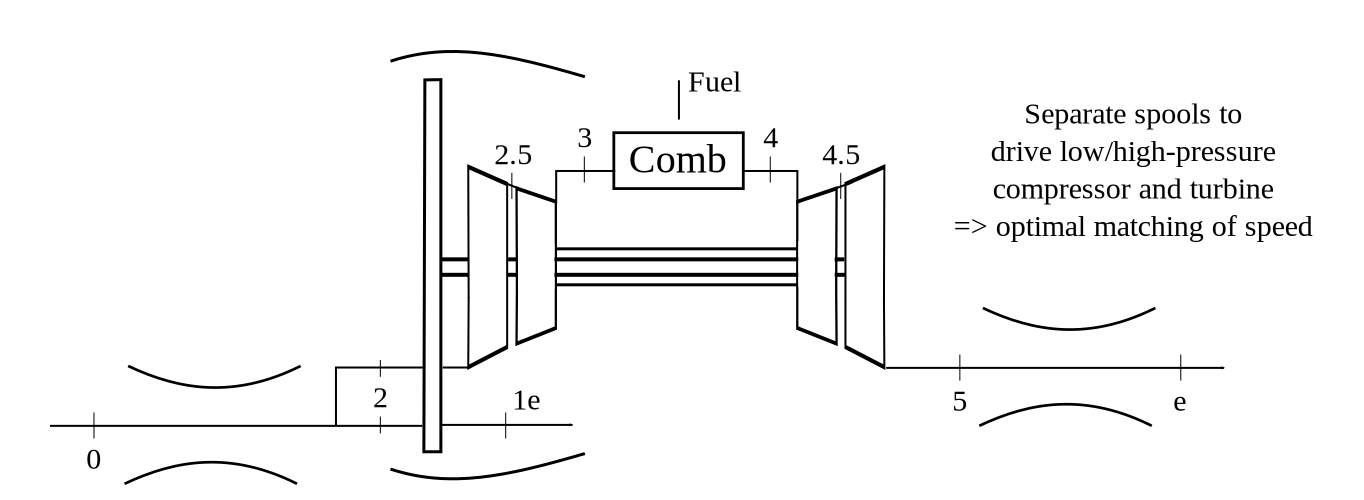
\includegraphics[width=0.9\textwidth, clip=, keepaspectratio]{multiSpoolTurbofan}}
    \caption{\label{FIG_MULTI_TURBOFAN}Multi-spool turbofan engine.}
\end{figure}
%==============================================================

\item Open rotor turboprop (\cref{FIG_TURBOPROP})

%==============================================================
\begin{figure}[!htb!]
 \centering
    {\includegraphics[width=0.82\textwidth, clip=, keepaspectratio]{turboprop}}
    \caption{\label{FIG_TURBOPROP}Turboprop engine.}
\end{figure}
%==============================================================

\item Low bypass-ratio turbofan with afterburner (\cref{FIG_TURBOFANAB})

%==============================================================
\begin{figure}[!htb!]
 \centering
    {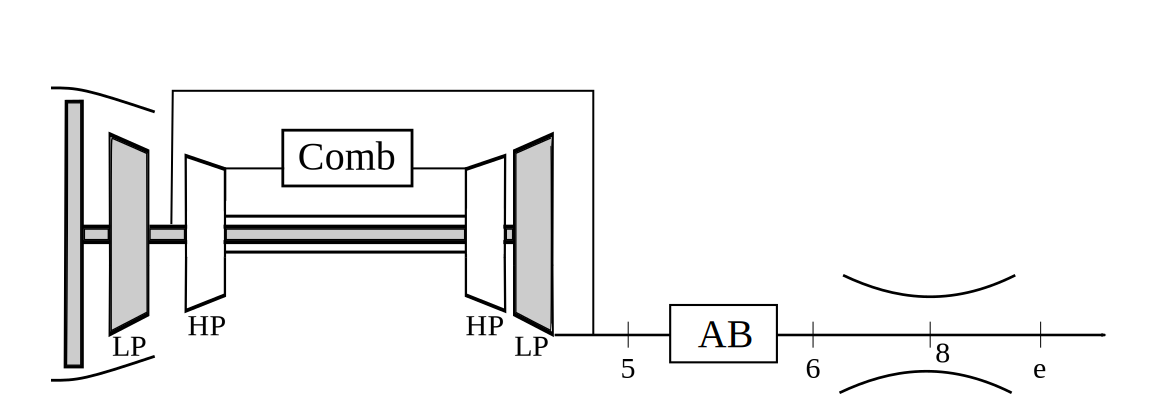
\includegraphics[width=0.82\textwidth, clip=, keepaspectratio]{turbofanAB}}
    \caption{\label{FIG_TURBOFANAB}Low bypass-ratio turbofan with afterburner (AB).}
\end{figure}
%==============================================================

\end{itemizePacked}
%%%%%%%%%%%%%%%%%%%%%%%%%%%%%%%%%%%%%%%%%%%%%%%%%%%%%%%%%%%%%
\subsubsection{Objectives of Engine Analysis}
%%%%%%%%%%%%%%%%%%%%%%%%%%%%%%%%%%%%%%%%%%%%%%%%%%%%%%%%%%%%%%
The objectives of engine analysis includes:
\begin{itemizePacked}
\item Estimate the best possible engine performance as a function of principle design parameters:
  \begin{itemizePacked}
  \item Maximum engine temperature
  \item Pressure ratio
  \item Flight speed
  \item Ambient conditions
  \end{itemizePacked}
\item Evaluate effects of departure from ideality in engine components:
  \begin{itemizePacked}
  \item Compressor
  \item Turbine
  \item Nozzle
  \end{itemizePacked}
\item Establish methods to enable the assessment of strategies for future performance increase.
\item Design components to match the engine performance (compressor and turbine).
\item Evaluate effects of engine performance on aircraft performances.
\end{itemizePacked}
The input for the engine design analysis includes:
\begin{itemizePacked}
\item Flight conditions: $\M_0,\, T_0, \,p_0,\, c_p$
\item Design parameters: $T_{04}$ (combustor exit temperature)
\item Component performances: $A_C,\, \eta_C,\, \eta_\text{comb},\, \eta_T$
\end{itemizePacked}
and the output or the design choices are $A_C,\, U_e,\, T,\, \dot{m}_F,\, f$.

%%%%%%%%%%%%%%%%%%%%%%%%%%%%%%%%%%%%%%%%%%%%%%%%%%%%%%%%%%%%%%
\subsection{Analysis of Turbojet Engines}
%%%%%%%%%%%%%%%%%%%%%%%%%%%%%%%%%%%%%%%%%%%%%%%%%%%%%%%%%%%%%%
Here we perform a basic analysis of turbojet engines. A schematic of this engine is shown in \cref{FIG_TURBOJET_ANALYSIS}.
%==============================================================
\begin{figure}[!htb!]
 \centering
    {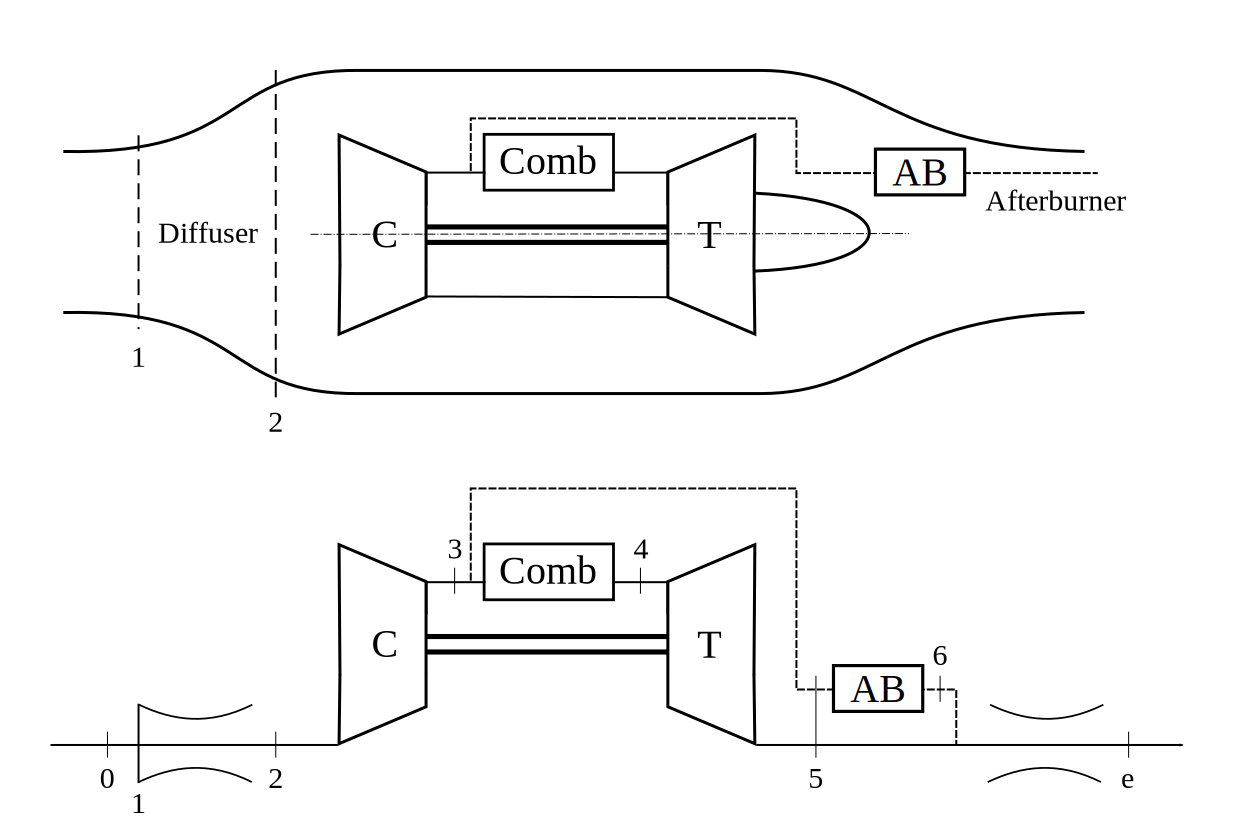
\includegraphics[width=0.82\textwidth, clip=, keepaspectratio]{turbojetAnalysis}}
    \caption{\label{FIG_TURBOJET_ANALYSIS}Schematic of a turbojet engine.}
\end{figure}
%==============================================================
The flow through this engine is described by the following processes:
\begin{itemizePacked}
\item 0 $\rightarrow$ 1: Air at freestream/flight condition is brought to intake condition (typically involving acceleration or deceleration of the flow-velocity)
\item 1 $\rightarrow$ 2: Decrease in air velocity as air passes through diffuser
\item 2 $\rightarrow$ 3: Compression of air in compressor
\item 3 $\rightarrow$ 4: ``Heating" of air by mixing and burning with fuel
\item 4 $\rightarrow$ 5: Expansion of air through turbine to extract technical work to drive compressor
\item (5 $\rightarrow$ 6): Further heating of air by combustion in afterburner
\item 5 $\rightarrow$ e: Acceleration of air through exhaust nozzle
\end{itemizePacked}
Some remarks on the afterburner:
\begin{itemizePacked}
\item The bypass flow is utilized for cooling and for providing excess air for combustion in the afterburner
\item The bypass flow is about 30--40\% or ``low bypass ratio".
\end{itemizePacked}

%%%%%%%%%%%%%%%%%%%%%%%%%%%%%%%%%%%%%%%%%%%%%%%%%%%%%%%%%%%%%%
\subsubsection{Ideal Brayton Cycle Analysis}
%%%%%%%%%%%%%%%%%%%%%%%%%%%%%%%%%%%%%%%%%%%%%%%%%%%%%%%%%%%%%%
To illustrate the analysis of an ideal Brayton cycle, we consider the flight conditions at $z$ = 7500 m, $T_0$ = 214.5 K, $p_0$ = 36.1 kPa, $\gamma$ = 1.4, and $M$~=~0.85. The overall pressure ratio for the compressor $p_{03}/p_{02} = 25$. For the combustor, we consider a heating value of  $Q_R = \text{LHV} = 45000$~kJ/kg$_\text{Fuel}$, and the combustor exit temperature is $T_{04}$ = 1500 K.

The $T$-$s$ diagram for the Ideal Brayton cycle is shown in \cref{FIG_IDEAL_BRAYTON}.

%==============================================================
\begin{figure}[!htb!]
 \centering
    {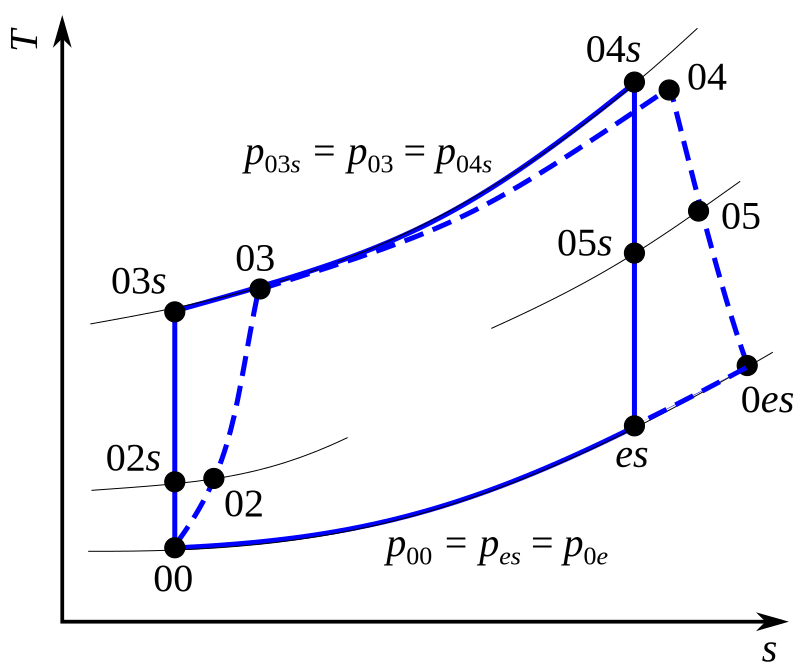
\includegraphics[width=0.52\textwidth, clip=, keepaspectratio]{braytonReal}}
    \caption{\label{FIG_IDEAL_BRAYTON}$T$-$s$ diagram of ideal and real Brayton cycle. Solid blue line for ideal Brayton cycle and dashed blue line for real Brayton cycle.}
\end{figure}
%==============================================================

%%%%%%%%%%%%%%%%%%%%%%%%%%%%%%%%%%%%%%%%%%%%%%%%%%%%%%%%%%%%%%
\subsubsection{Real Brayton Cycle Analysis}
%%%%%%%%%%%%%%%%%%%%%%%%%%%%%%%%%%%%%%%%%%%%%%%%%%%%%%%%%%%%%%

%==============================================================
\begin{figure}[!htb!]
 \centering
    {\includegraphics[width=0.88\textwidth, clip=, keepaspectratio]{turbojetAnalysis_MEffects}}
    \caption{\label{FIG_turbojetAnalysis_MEffects}Thrust specific fuel consumption and specific thrust as a function of Mach number and $\pi_C$.}
\end{figure}
%==============================================================

%==============================================================
\begin{figure}[!htb!]
 \centering
    {\includegraphics[width=0.88\textwidth, clip=, keepaspectratio]{turbojetAnalysis_TSFC}}
    \caption{\label{FIG_turbojetAnalysis_TSFC}Thrust specific fuel consumption as a function of temperature and $\pi_C$.}
\end{figure}
%==============================================================

%==============================================================
\begin{figure}[!htb!]
 \centering
    {\includegraphics[width=0.88\textwidth, clip=, keepaspectratio]{turbojetAnalysis_SpecificThrust}}
    \caption{\label{FIG_turbojetAnalysis_SpecificThrust}Specific thrust as a function of temperature and $\pi_C$.}
\end{figure}
%==============================================================

For practical turbojets, we need to consider non-idealities that arise from irreversibility due to:
\begin{itemizePacked}
\item Friction
\item Mixing
\item Pressure drop
\item Flow separation
\end{itemizePacked}
%The real Brayton cycle is also shown in \cref{FIG_IDEAL_BRAYTON} in comparison with the ideal Brayton cycle.
To account for such effects we introduce the {\it adiabatic efficiency} $\eta$:
\begin{itemizePacked}
\item Diffuser: 
\begin{equation}
  \eta_D = \f{h_{02s}-h_{0}}{h_{02}-h_{0}}\,;
\end{equation}
\item Compressor:
\begin{equation}
  \eta_C = \f{h_{03s}-h_{02}}{h_{03}-h_{02}}\,;
\end{equation}
\item Turbine:
\begin{equation}
  \eta_T = \f{h_{04}-h_{05}}{h_{04}-h_{05s}}\,;
\end{equation}
\item Nozzle:
\begin{equation}
  \eta_N = \f{h_{05}-h_{0e}}{h_{05}-h_{es}}\,.
\end{equation}
\end{itemizePacked}
Typical values for the adiabatic efficiencies are $\eta_D = 0.7-0.9$, $\eta_C = 0.85-0.9$, $\eta_\text{comb} = 0.9-0.95$, $\eta_T = 0.97-0.99,$ and $\eta_N = 0.95-0.98.$

To include these efficiencies in our analysis, we consider the following numerical values:
\begin{itemizePacked}
\item Diffuser: $\eta_D = 0.95$
\item Compressor: $\eta_C = 0.87$
\item Combustor: $\eta_\text{comb} = 1.0$
\item Turbine: $\eta_T = 0.91$
\item Nozzle: $\eta_N = 0.98$
\end{itemizePacked}
The pressure drop $p_{04}/p_{03} = 0.96 = \pi_\text{comb}$. With this, we can perform the engine analysis. For this, we proceed successively through the engine, and consider each component.

\begin{itemizePacked}
\item Compressor inlet condition:
\begin{equation}
T_{02} = T_0 \left(1+\f{\gamma_D-1}{2}\text{M}_0^2 \right)\,.
\end{equation}
From
\begin{equation}
\eta_D = \f{h_{02s}-h_{0}}{h_{02}-h_{0}} = \f{T_{02s}-T_{0}}{T_{02}-T_{0}}\,,
\end{equation}
and rearrange to solve for the isentropic stagnation temperature at stage 2
\begin{equation}
\f{T_{02s}}{T_{0}} = 1+\eta_D\left( \f{T_{02}}{T_{0}} -1 \right)\,.
\end{equation}
Since $p_{02} = p_{02s}$,
\begin{equation}
\f{p_{02s}}{p_{0}} = \f{p_{02}}{p_{0}} = \left( \f{T_{02s}}{T_{0}} \right)^\f{\gamma_D}{\gamma_D-1} = \left[1+\eta_D\left( \f{T_{02}}{T_{0}} -1 \right) \right]^\f{\gamma_D}{\gamma_D-1}\,,
\end{equation}
where $\gamma_D$ is the specific heat ratio in the diffuser.
\item Compressor outlet condition:
\begin{equation}
p_{03} = p_{02} \pi_C\,.
\end{equation}
From 
\begin{equation}
\eta_C = \f{T_{03s}-T_{02}}{T_{03}-T_{02}} \quad \text{and} \quad \f{T_{03s}}{T_{02}} = \left( \f{p_{03}}{p_{02}} \right)^\f{\gamma_C-1}{\gamma_C}\,,
\end{equation}
we have
\begin{eqnarray}
  \f{T_{03}}{T_{02}} &=& 1+\f{1}{\eta_C}\left( \pi_C^\f{\gamma_C-1}{\gamma_C} -1 \right)\;,\\
  \f{p_{03}}{p_{02}} &=& \pi_C
\end{eqnarray}
\item Combustor (fuel/air ratio): 
Typically $T_{04}$ is specified and determined by material properties of the turbine. From the overall conservation: 
$\left.{dh}\right|_3^4 = \Delta \dot{Q}$, we have (here we assume that the fuel has the same temperature as the air at the combustor inlet):
\begin{eqnarray}
(\dot{m}_A+\dot{m}_F)h_{04} - (\dot{m}_A +\dot{m}_F) h_{03} &=& \dot{m}_F \text{LHV}\,,\\
(1+f)(h_{04} - h_{03}) &=& f \text{LHV}\,,
\end{eqnarray}
where $h_{03} = c_p (T_{03}-T_\text{ref})$ and $h_{04} = c_p (T_{04}-T_\text{ref})$. Solving for the fuel-air ratio $f$:
\begin{eqnarray}
  f &=& \f{\f{T_{04}}{T_{03}}-1}{\f{\text{LHV}}{c_p T_{03}}-\left( \f{T_{04}}{T_{03}}-1 \right)}\,,\\
  p_{04} &=& p_{03} \pi_\text{comb}\,.
\end{eqnarray}
\item Turbine exit condition:
The work extracted from the turbine is used to drive the compressor. For an adiabatic system: $dh = - \delta w_t$,
\begin{eqnarray}
(\dot{m}_A+\dot{m}_F)c_p (T_{05}-T_{04}) &=& -\dot{m}_A c_p (T_{03}-T_{02})\,,\\
T_{05} &=& T_{04} - \f{c_p^C (T_{03}-T_{02})}{(1+f) c_p^T}\,,\\
T_{05} &=& T_{04} - (T_{03}-T_{02})\,,
\end{eqnarray}
for $f \sim 0$ and $c_p^T = c_p^C$.
With the adiabatic efficiency
\begin{equation}
\eta_T = \f{h_{04}-h_{05}}{h_{04}-h_{05s}} = \f{\f{T_{05}}{T_{04}}-1}{\f{T_{05s}}{T_{04}}-1}\,,
\end{equation}
we have
\begin{align}
\f{T_{05s}}{T_{04}} &= 1+\f{1}{\eta_T} \left( \frac{T_{05}}{T_{04}}-1 \right)\,,\\
\f{p_{05}}{p_{04}} &= \left(\f{T_{05s}}{T_{04}}\right)^\f{\gamma^T}{\gamma^T-1} = \left[ 1+\frac{1}{\eta_T} \left( \f{T_{05}}{T_{04}}-1 \right) \right]^\f{\gamma^T}{\gamma^T-1}\,. \label{eq:p05_over_p04}
\end{align}
\item Nozzle exit condition: From enthalpy conservation
\begin{eqnarray}
\f{1}{2}u_e^2 &=& h_{05} - h_e = \eta_p(h_{05}-h_{es})\,,\\
\f{1}{2}u_e^2 &=& \eta_p c_p T_{05}(1-\f{T_{es}}{T_{05}})\,,
\end{eqnarray}
and solving for $u_e$
\begin{equation}
u_e = \sqrt{2 \eta_p c_p T_{05}\left[1- \left(\f{p_{es}}{p_{05}}\right)^\f{\gamma_N-1}{\gamma_N} \right]}
\end{equation}
for an unchoked nozzle flow.
\end{itemizePacked}

For the performance analysis, we are mostly interested in the following two parameters:
\begin{itemizePacked}
\item Specific thrust:
\begin{equation}
  \f{T}{\dot{m}_A} = [(1+f)U_e - U_0]\,;
\end{equation}
\item Specific fuel consumption:
\begin{equation}
  \f{\dot{m}_F}{T} = \f{f}{[(1+f)U_e-U_0]}\,.
\end{equation}
\end{itemizePacked}

%%==============================================================
%\begin{figure}[!htb!]
% \centering
%   \subfigure[\label{FIG_REAL_BRAYONR_ANALYSIS_MO}Static condition (M = 0).]
%    {\includegraphics[width=0.42\textwidth, clip=, keepaspectratio]{piCM0} \quad}
%   \subfigure[\label{FIG_REAL_BRAYONR_ANALYSIS_M085}Cruise thrust (M = 0.85).]
%    {\includegraphics[width=0.42\textwidth, clip=, keepaspectratio]{piCM085}}
%   \subfigure[\label{FIG_REAL_BRAYONR_ANALYSIS_M2}Supersonic cruise thrust (M = 2).]
%    {\includegraphics[width=0.42\textwidth, clip=, keepaspectratio]{piCM2}}
%    \caption{\label{FIG_REAL_BRAYONR_ANALYSIS}Specific thrust and specific fuel consumption as a function of $\pi_C$ at different Mach numbers.}
%\end{figure}
%%==============================================================

Performing the real-Brayton-cycle analysis for a range of pressure ratios and Mach-numbers provides information about the engine performance. These results are schematically illustrated in \crefrange{FIG_turbojetAnalysis_MEffects}{FIG_turbojetAnalysis_TSFC}:
\begin{itemizePacked}
\item For given $\M$ and $T_{04}$, $\pi_C$ for the minimum fuel consumption and the maximum thrust do not coincide. Both $\dot{m}_F$ and $T_{04}$ require consideration for selecting best compressor pressure ratio.
\item Increasing $T_{04}$ substantially improves thrust, maximum thrust $T_\text{max} \sim 1700$~K is well below adiabatic flame temperature. Blade cooling and high-temperature alloys are required to facilitate thermal stability at these high combustor exit temperatures.
\item Increase $T_{04}$ can affect $\dot{m}_F/T$.
\item $\pi_C$ for supersonic flight is much less than that for subsonic condition (limit of ramjet).
\end{itemizePacked}

%%%%%%%%%%%%%%%%%%%%%%%%%%%%%%%%%%%%%%%%%%%%%%%%%%%%%%%%%%%%%%
\subsection{Analysis of Turbofan Engines}
%%%%%%%%%%%%%%%%%%%%%%%%%%%%%%%%%%%%%%%%%%%%%%%%%%%%%%%%%%%%%%
From the general performance analysis (see \cref{eqn:etaPropulsive}), we found that the overall efficiency is related to the propulsive and thermal efficiency, $\eta_o = \eta_p \eta_{th}$, with
\[
\eta_p = \f{2}{1+\f{U_e}{U_0}}\,.
\]
Therefore, for a fixed $\eta_{th}$, we can maximize $\eta_p$ and $\eta_o$ by letting $U_e \rightarrow U_0$. For a turbojet engine, $U_e$ is defined by the exit enthalpy and nozzle design. Considering different engine-design concepts, the relation between $\eta_p$ and $U_0$ is shown in \cref{FIG_RELATION_U0ETAP}.

%==============================================================
\begin{figure}[!htb!]
 \centering
    {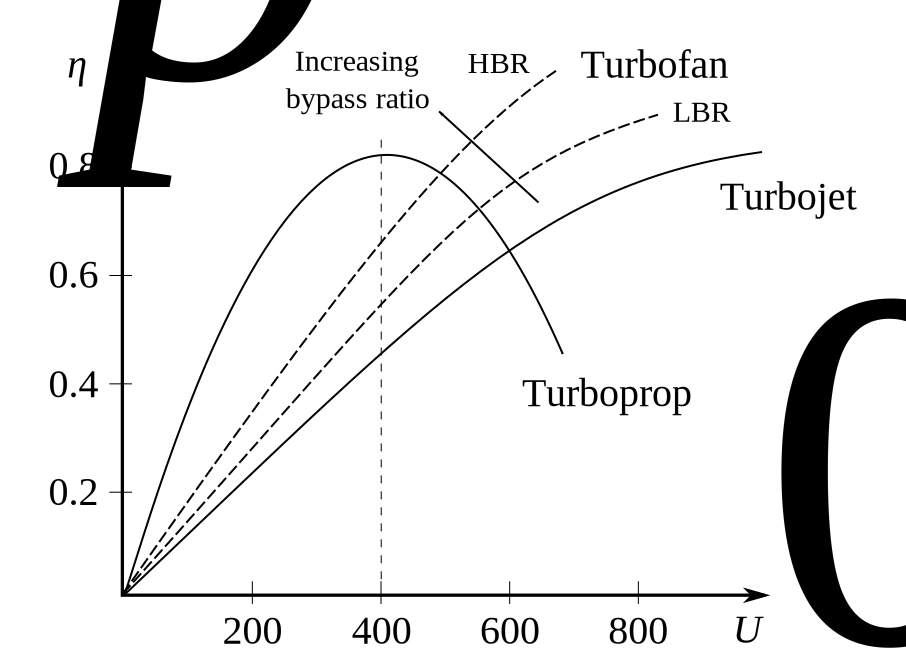
\includegraphics[width=0.58\textwidth, clip=, keepaspectratio]{relationU0Etap}}
    \caption{\label{FIG_RELATION_U0ETAP}Relation between $\eta_p$ and $U_0$ for different types of engines.}
\end{figure}
%==============================================================

%==============================================================
\begin{figure}[!htb!]
 \centering
    {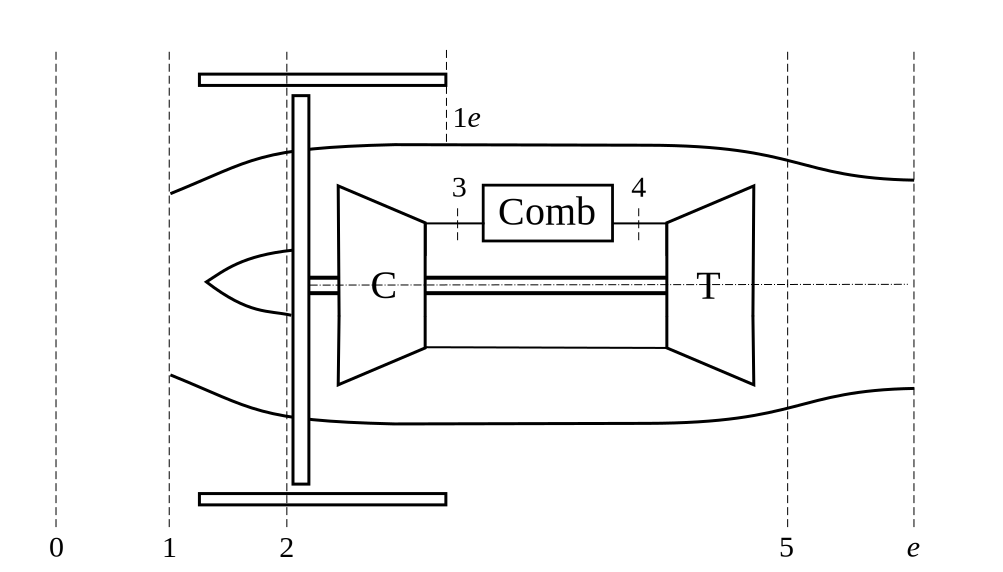
\includegraphics[width=0.72\textwidth, clip=, keepaspectratio]{turbofanAnalysis}}
    \caption{\label{FIG_TURBOFAN_ANALYSIS}Schematic of the turbofan engine.}
\end{figure}
%==============================================================

For a turboprop engine or unducted fan-engine, we obtain the highest bypass ratio since $\beta\to\infty$. However, these engines are limited by the flight Mach number to less than 0.5 (so that the blade tip-speed doesn't exceed supersonic condition). For $\M > 0.5$, the engine will become noisy and we will have supersonic tip velocity, shock waves and flow separation. 

Recall the thrust equation for a turbofan engine (\cref{FIG_TURBOFAN_ANALYSIS})
\begin{equation}
   T = \dot{m}_{A\,,C} \left[ (1+f) U_e + \beta U_{1e} - (1+\beta) U_0 \right] \, \text{.}
\end{equation}
We have
\begin{equation}
  \text{TSFC} = \f{\dot{m}_F}{T} = \f{f}{(1+f)U_e+\beta U_{1e} - (1+\beta)U_0}\,.
\end{equation}

The analysis of a turbofan engine follows that of the turbojet engine with some additional component analysis:
\begin{itemizePacked}
\item Fan inlet condition: Air is supplied from the diffusor, so that pressure and temperature are identical to that of the core flow
\begin{eqnarray}
T_{012} &=& T_{02}\,,\\
p_{012} &=& p_{02}\,.
\end{eqnarray}
\item Fan outlet condition: Define fan pressure rate $\pi_F = \f{p_{018}}{p_{02}}$ and fan adiabatic efficiency $\eta_F = \f{h_{018s}-h_{012}}{h_{018}-h_{012}}$, we have
\begin{eqnarray}
p_{018} &=& p_{02}\pi_F\,,\\
T_{018} &=& T_{02}\left[1+\f{1}{\eta_F}\left(\pi_F^\f{\gamma_F-1}{\gamma_F}-1\right)\right]\,.
\end{eqnarray}
\item Fan nozzle exit condition: The evaluation of the fan-nozzle exit velocity directly follows from the enthalpy conservation:
\begin{equation}
  u_{1e} = \sqrt{2\eta_F c_p T_{018} \left[1-\left(\f{p_0}{p_{018}}\right)^\f{\gamma_F-1}{\gamma_F}\right]}\,.
\end{equation}
\item Turbine exit condition: Considering work-balance between compressor and turbine provides a relation to evaluate the turbine work that is required to drive the compressor and fan:
\begin{equation}
(\dot{m}_{A,C}+\dot{m}_F)c_p^T (T_{05}-T_{04}) = -\dot{m}_{A,C} c_p^C (T_{03}-T_{02}) -\dot{m}_{A,B} c_p^F (T_{018}-T_{02})\,.
\end{equation}
With $\beta = \dot{m}_{A,B}/\dot{m}_{A,C}$, we can simplify:
\begin{eqnarray}
(1+f) c_p^T (T_{05}-T_{04}) &=& - c_p^C (T_{03}-T_{02}) -\beta c_p^F (T_{018}-T_{02})\,,\\
T_{05} &=& T_{04} - \f{c_p^C(T_{03}-T_{02}) + \beta c_p^F (T_{018}-T_{02})}{(1+f)c_p^T}\,,
\end{eqnarray}
with $f \sim 0$ and $c_p = c_p^T = c_p^C$, we have
\begin{equation}
	T_{05} = T_{04} - (T_{03}-T_{02})-\beta(T_{018}-T_{02}).
\end{equation}
The pressure at the turbine exit can be obtained using the same expression as shown in~\cref{eq:p05_over_p04} for the turbojet.
% \begin{eqnarray}
% T_{05} &=& T_{04} - (T_{03}-T_{02})-\beta(T_{08}-T_{02})\,,\\
% \f{p_{05}}{p_{04}} &=& \left[1+\f{1}{\eta_T}\left(\f{T_{05}}{T_{04}}-1\right)^\f{\gamma_T}{\gamma_T-1}\right]\,.
% \end{eqnarray}
\item Nozzle exit condition:
\[
  u_e = \sqrt{2 \eta_N c_p^N T_{05} \left[ 1 - \left(\f{p_{es}}{p_{05}}\right)^\f{\gamma_N-1}{\gamma_N}\right]}\,,
\]
where $p_{es} = p_0$.
\end{itemizePacked}
Some remarks are in order:
\begin{itemizePacked}
\item The main benefit of higher bypass ratios is achieved at take-off condition
\item The benefit of the higher bypass ratio reduces with increasing flight Mach number and altitude
\item No benefits of bypass ratio at trans/supersonic conditions; losses due to the increase engine cross-section and shock losses exceed the gain that is achieved by the bypass ratio
\item For aircraft operating at sub/supersonic conditions, it is essential to optimize the design of the bypass ratio
\item Criteria for limitation on bypass ratio:
  \begin{itemizePacked}
  \item Speed mismatch between fan and turbine
  \item Weight consideration
  \item Aerodynamic drag
  \item Gear box design.
  \end{itemizePacked}
\end{itemizePacked}

%%%%%%%%%%%%%%%%%%%%%%%%%%%%%%%%%%%%%%%%%%%%%%%%%%%%%%%%%%%%%%
\subsection{Examples of Turbofan Engines}
%%%%%%%%%%%%%%%%%%%%%%%%%%%%%%%%%%%%%%%%%%%%%%%%%%%%%%%%%%%%%%
This section provides a summary of relevant turbofan engines that are currently employed as propulsion systems for military and civil aircraft.

%%%%%%%%%%%%%%%%%%%%%%%%%%%%%%%%%%%%%%%%%%%%%%%%%%%%%%%%%%%%%%
\subsubsection{Military Aircraft Engines}
%%%%%%%%%%%%%%%%%%%%%%%%%%%%%%%%%%%%%%%%%%%%%%%%%%%%%%%%%%%%%%

%%%%%%%%%%%%%%%%%%%%%%%%%%%%%%%%%%%%%%%%%%%%%%%%%%%%%%%%%%%%%%
\paragraph{Pratt \& Whitney F135:}
%%%%%%%%%%%%%%%%%%%%%%%%%%%%%%%%%%%%%%%%%%%%%%%%%%%%%%%%%%%%%%
The Pratt \& Whitney F135 propulsion system (\cref{FIG_PW135_SCHEMATIC_FIG}) is the engine of choice for the advanced, single-engine tactical fighter F-35 (Joint Strike Fighter, JSF), which has been developed by Lockheed Martin. The F-35 has unique capabilities for land-based conventional takeoff and landing (CTOL), carrier-variant takeoff and landing (CVTOL) and short takeoff and vertical landing (STOVL). The F135 propulsion system has already proved that it can meet these diverse requirements. As planned, the new F-35 JSF aircraft will replace the F-16 Fighting
Falcon, A-10 Thunderbolt II, AV-8B Harrier, and F/A-18 Hornet.

%==============================================================
\begin{figure}[!htb!]
 \centering
   \subfigure[\label{FIG_PW135_SCHEMATIC}Engine schematic.]
    {\includegraphics[width=0.59\textwidth, clip=, keepaspectratio]{pwF135Schematic}}
   \subfigure[\label{FIG_PW135_IMAGE}Engine assembly.]
    {\includegraphics[width=0.4\textwidth, clip=, keepaspectratio]{pwF135Engine}}
    \caption{\label{FIG_PW135_SCHEMATIC_FIG}Schematic and image of Pratt \& Whitney's F135 engine (source: \url{www.pw.utc.com}).}
\end{figure}
%==============================================================
The F135 is an evolution of the F119-PW-100, a technologically advanced turbofan that powers the Air Force's F/A-22 Raptor. It integrates the proven F119 core (see Paragraph \ref{SUBSEC_F119}), a high-performance six-stage compressor and single-stage turbine unit with a new low-pressure spool. In addition, the propulsion system features advanced prognostic and on-condition management systems that provide maintenance awareness, autonomic logistic support, and automatic field data and test systems. All line-replaceable components (LRCs) can be removed and replaced with a set of six common hand tools. The first production propulsion system for operational service was scheduled for delivery in 2007.

Engine Characteristics: 
\begin{itemize}[noitemsep=2pt,topsep=0pt]
 \item {\it Thrust}: 43,000 lbf (191.35 kN).
 \item {\it Intake}: Ring of 21 fixed radial guide vanes, with hinged trailing flaps, which carry front LP bearing.
 \item {\it Fan (LP Compressor)}: Three integrally bladed rotors, derived from F119 but with new features giving greater mass flow with higher pressure ratio, improved stability, maximum resistance to bird and other impact damage, and minimum signature. Rotors 2 and 3 are made of  flank-milled titanium alloy.
 \item {\it  HP Compressor}: Six-stage compressor derived from F119, rotating in opposition to LP spool. Split forward case in titanium alloy housing two stages of asymmetric variable-incidence guide vanes (stators). Cast nickel-alloy rear stators grouped in segments in titanium-alloy ring casing of high creep strength. All stators integrally bladed, either flat-milled like the fan or high-speed milled.
 \item {\it  Combustor}: Short annular diffuser/combustor, derived from F119. Outer casing about 762 mm in both diameter and length, weighing 91 kg  including HPT nozzle ring (lighter and less costly than in previous P\&W fighter engines), handling airflow at 4,150 kPa  at 649$^\circ$C, and containing air-conditioning connections. The combustion chamber is 510 mm in diameter and 230 mm long, weighting 32 kg. Liner with impingement and film cooling containing Floatwall ceramic-coated nickel-based cast segments, each containing ``thousands of holes'', which ``float'' from their anchored location. Intense combustion with fuel/air ratio 20 per cent higher than in F100 engine to give near-record gas temperature exceeding 2,200$^\circ$C (4,000F).
 \item {\it  HP Turbine}: High-pressure single stage turbine based on F119, with advanced airfoil coating and cooling derived from F119, but with cooling airflow doubled. Impingement cooling augmented by closing down rear stator angles. Nozzle ring c120 organic-matrix vanes with wall thickness 0.5 mm. The rotor comprises a main disk, miniature disk and cover plates, all incorporating the same high-strength powder-metallurgy (sintered) high-rotor blades of second-generation single-crystal Ni-based alloy, with advanced outer air
seals. Unit diameter 914 mm, length 356 mm, weight 183 kg. The HPT rotates at speeds exceeding 15,000 rpm, generating 47,725 kW from gas at just over 1,649$^\circ$C, cooled by air supplied at 538$^\circ$C from the HPC. To minimize pressure loss the rotor blades are
cooled by Tangential On-Board Injection (TOBI), each blade being a complex casting with multiple cooling passages. Growth in blade-tip diameter is controlled by a unique slow-responding thermally isolated support ring in materials selected for their low thermal expansion, giving passive clearance control through the normal engine-operating range.
 \item {\it  LP Turbine}: Two-stage design giving significantly greater shaft power than the single-stage LPT of the F119. Rotates in opposition to the HP turbine. Typical of the simplified design of the F135 are the main shaft bearings, (see note under HP compressor), and it is possible that the full production F135 may have a corrosion-resistant ceramic (silicon nitride) bearing.
 \item {\it  Afterburner}: Advanced flame-holder system. Fully variable convergence-divergence nozzle, with 15 hydraulically driven hinged flaps, controlling propulsive jet at 621 kPa at up to 1,927$^\circ$C. In the F135-PW-600 the complete nozzle can vector through 95$^\circ$ in 2.5 s to give 80.34 kN lift force for STOVL, driven by a Smiths Aerospace actuation system.
\end{itemize}

%==============================================================
\begin{table}[!htb!]
  \centering
\begin{tabular}{|p{0.25\textwidth}|p{0.7\textwidth}|}\hline
Variants & F135-PW-100: F-35A Conventional take-off and landing\\
         & F135-PW-400: F-35C Carrier variant\\
         & F135-PW-600: F-35B Short take-off vertical landing\\
Dimensions & F135-PW-100/400: Length 5,588 mm, diameter 1,295 mm\\
           & F135-PW-600: Length 9,373 mm, diameter 1,295 mm\\
Maximum thrust &43,000 lbf (191.35 kN)\\
TSFC& 0.886 lb/(lbf-h), 25 mg/(N-s) (without afterburner)\\
Thrust-to-weight ratio& 11.5\\
Implementation & F-35\\\hline
\end{tabular}
  \caption{\label{TAB_F135}Engine specification for F135.}
\end{table}
%==============================================================

%%%%%%%%%%%%%%%%%%%%%%%%%%%%%%%%%%%%%%%%%%%%%%%%%%%%%%%%%%%%%%
\paragraph{\label{SUBSEC_F119}Pratt \& Whitney F119:}
%%%%%%%%%%%%%%%%%%%%%%%%%%%%%%%%%%%%%%%%%%%%%%%%%%%%%%%%%%%%%%
Pratt \& Whitney's F119 turbofan engine, the world's most technologically advanced aircraft engine in
production, meets the need for greater speed and lower weight for new military weapon systems. In the
35,000 pound thrust class, the engine is a dual spool, counter-rotating turbofan that enables aircraft
operation at supersonic speeds for extended periods without thrust augmentation.

%==============================================================
\begin{figure}[!htb!]
 \centering
    {\includegraphics[width=0.85\textwidth, clip=, keepaspectratio]{pwF119Schematic}}
    \caption{\label{FIG_PW119}Schematic of Pratt \& Whitney's F119 engine (source: \url{www.pw.utc.com}).}
\end{figure}
%==============================================================

The F119 is equipped with a number of advanced technologies: Its three-stage fan has shroudless titanium fan blades and is powered by a single-stage low-pressure turbine. The engine's core has an aerodynamically efficient six-stage compressor driven by a single-stage high-pressure turbine featuring the next generation of single-crystal super-alloy blades with improved cooling management. The robust, but compact, high-pressure compressor features integrally bladed rotor disks for improved durability. The engine delivers unparalleled aircraft maneuverability with its unique two-dimensional thrust vectoring exhaust nozzle. This convergent/divergent nozzle vectors thrust 20$^\circ$ either up or down. Nozzle position management is automatically controlled by the full-authority digital electronic control (FADEC), which controls hundreds of other engine and aircraft operating parameters. The FADEC also features advanced diagnostic and on-condition management systems for maintenance awareness, autonomic logistics support, and automatic field data and test systems.
%==============================================================
\begin{table}[!htb!]
  \centering
\begin{tabular}{|p{0.25\textwidth}|p{0.7\textwidth}|}\hline
Engine Type &  Twin-Spool, augmented turbofan\\
Thrust & 35,000 lb Thrust class\\
Compressor & Twin-spool/Counter-rotating/Axial flow\\
Combustor & Annular\\
Turbine & Axial flow/Counter-rotating\\
Nozzle & Two Dimensional Vectoring Convergent/Divergent\\
Implementation& F/A-22 Raptor\\\hline
\end{tabular}
  \caption{\label{TAB_F119}Specification of F119 engine.}
\end{table}
%==============================================================

%%%%%%%%%%%%%%%%%%%%%%%%%%%%%%%%%%%%%%%%%%%%%%%%%%%%%%%%%%%%%%
\paragraph{Pratt \& Whitney F100:}
%%%%%%%%%%%%%%%%%%%%%%%%%%%%%%%%%%%%%%%%%%%%%%%%%%%%%%%%%%%%%%
Pratt \& Whitney's family of F100 engines is the mainstay of air forces worldwide. With more than 6,900 engines produced and over 16 million flight hours, the F100 is the safest and most reliable fighter engine in the world. It is the only Increased Performance Engine (IPE) operationally matured in both the F-15E and F-16 Block 52 aircraft. Using technology developed from the F119 and F135 engine programs for the F/A-22 Raptor and F-35 Joint Strike Fighter, the current production PW-229 incorporates modern turbine materials, cooling management techniques, compressor aerodynamics and electronic controls.

%==============================================================
\begin{figure}[!htb!]
 \centering
%   \subfigure[\label{FIG_PW100_SCHEMATIC}Engine schematic.]
    {\includegraphics[width=0.85\textwidth, clip=, keepaspectratio]{pwF100-PW-229}}
%   \subfigure[\label{FIG_PW100_TEST_STAND}Teststand.]
%    {\includegraphics[width=0.34\textwidth, clip=, keepaspectratio]{pwF100TestStand}}
    \caption{\label{FIG_PW100_SCHEMATIC}Schematic of Pratt \& Whitney's F100 engine (source: \url{www.pw.utc.com}).}
\end{figure}
%==============================================================

%==============================================================
\begin{table}[!htb!]
  \centering
\begin{tabular}{|p{0.25\textwidth}|p{0.7\textwidth}|}\hline
Engine Thrust & 23,770--29,160 lb\\
Dimensions & Weight: 3,740 lb, length: 191 in, diameter: 46.5 in\\
Bypass Ratio& 0.36\\
Overall Pressure Ratio& 25--32\\
Implementation& F-15, F-16\\\hline
\end{tabular}
  \caption{\label{TAB_F100}Specification of F100 engine.}
\end{table}
%==============================================================

%%%%%%%%%%%%%%%%%%%%%%%%%%%%%%%%%%%%%%%%%%%%%%%%%%%%%%%%%%%%%%
\subsubsection{Civil Aircraft Engines}
%%%%%%%%%%%%%%%%%%%%%%%%%%%%%%%%%%%%%%%%%%%%%%%%%%%%%%%%%%%%%%

%%%%%%%%%%%%%%%%%%%%%%%%%%%%%%%%%%%%%%%%%%%%%%%%%%%%%%%%%%%%%%
\paragraph{Pratt \& Whitney JT9D:}
%%%%%%%%%%%%%%%%%%%%%%%%%%%%%%%%%%%%%%%%%%%%%%%%%%%%%%%%%%%%%%
These engines opened a new era in commercial aviation: the high-bypass-ratio engine to power wide-bodied aircraft. Although production ended in 1990, Pratt \& Whitney continues to support the JT9D family. Upgrade programs are in place to enable operators to improve durability, increase thrust and reduce noise. 
%==============================================================
\begin{table}[!htb!]
  \centering
\begin{tabular}{|p{0.25\textwidth}|p{0.7\textwidth}|}\hline
Dimensions & Fan tip diameter: 93.4 in, Length: 132.7 in\\
Takeoff thrust & 48,000--56,000 lb\\
Bypass ratio & 0.36\\
Overall pressure ratio& 26.7\\
Fan pressure ratio& 1.67\\
Implementation& Boeing \{747,767\},  Airbus \{A300,A310\}, McDonnell Douglas DC-10\\\hline
\end{tabular}
  \caption{\label{TAB_JT9D}Engine characteristics of PW-JT9D engine.}
\end{table}
%==============================================================

%%%%%%%%%%%%%%%%%%%%%%%%%%%%%%%%%%%%%%%%%%%%%%%%%%%%%%%%%%%%%%
\paragraph{Pratt \& Whitney PW4000:}
%%%%%%%%%%%%%%%%%%%%%%%%%%%%%%%%%%%%%%%%%%%%%%%%%%%%%%%%%%%%%%
Today's PW4000 meets all current and anticipated emissions and noise regulations with margin. For a further reduction in emissions -- especially NO$_x$ -- TALON (Technology for Advanced Low NO$_x$) combustor technology is now available as an option. Derived from the 112-inch fan model, TALON has segmented, replaceable liner panels for easy maintainability and air blast fuel nozzles for excellent fuel
atomization and mixing.

%==============================================================
\begin{figure}[!htb!]
 \centering
    {\includegraphics[width=0.75\textwidth, clip=, keepaspectratio]{pw4000}}
    \caption{\label{FIG_PW4000}Cutaway of PW 4000 (source: \url{www.pw.utc.com}).}
\end{figure}
%==============================================================

%==============================================================
\begin{table}[!htb!]
  \centering
\begin{tabular}{|p{0.25\textwidth}|p{0.7\textwidth}|}\hline
Thrust range& 52,000--62,000 lb\\
Dimensions & Fan diameter: 94 in, Length: 132.7 in\\
Bypass ratio& 4.8--5.1\\
Overall pressure ratio & 27.5--32.3\\
Fan pressure ratio&  1.65--1.80\\
Implementation& Boeing \{747-400,767-200/300\},  Airbus \{A300-600,A310-300\}, McDonnell Douglas MD-11\\\hline
\end{tabular}
  \caption{\label{TAB_PW4000}Engine characteristics of PW 4000 engine.}
\end{table}
%==============================================================

%%%%%%%%%%%%%%%%%%%%%%%%%%%%%%%%%%%%%%%%%%%%%%%%%%%%%%%%%%%%%%
\paragraph{General Electric GE90:}
%%%%%%%%%%%%%%%%%%%%%%%%%%%%%%%%%%%%%%%%%%%%%%%%%%%%%%%%%%%%%%
The GE90 represents GE's investment in the future of wide-body aircraft. Over the past two decades, GE's CF6 and CFM56\footnote{CFM56 engines are produced by CFM International, a 50/50 joint company between Snecma Moteurs and General Electric Company} engines have been chosen to power more than 50 percent of all new aircraft ordered with a capacity of 100 passengers or more. The GE90 combines the best proven technology from these engine programs, NASA and military programs with advanced technology to provide a highly reliable, fuel-efficient powerplant for the next generation of wide-body aircraft.

Originally certified in 1995 at 84,700 pounds of thrust, today's GE90 engines power newer, more advanced Boeing 777 aircraft capable of flying farther, faster and more efficiently than their predecessors. The most recent derivative of the GE90, the GE90-115B, is the sole powerplant for Boeing's longer-range 777-300ER and 777-200LR aircraft. The GE90-115B is certified at 115,000 lbs of thrust and has broken a number of aviation records. The Guinness Book of World Records recognized the engine as the ``World's Most Powerful Commercial
Jet Engine'' in 2001 after it recorded an amazing 123,000 lbs of steady-state thrust while undergoing initial ground testing. In late 2002, the engine shattered its original record by reaching 127,900 lbs of thrust during required certification testing.

%==============================================================
\begin{figure}[!htb!]
 \centering
   \subfigure[\label{FIG_GE90_SCHEM}Engine schematic.]
    {\includegraphics[width=0.54\textwidth, clip=, keepaspectratio]{ge90-115BSchematic}}
   \subfigure[\label{FIG_GE90}Engine assembly.]
    {\includegraphics[width=0.45\textwidth, clip=, keepaspectratio]{ge90-115BAssembly}}
    \caption{\label{FIG_PW100_SCHEMATIC_FIG}Schematic and image of GE90-115B engine (source: \url{www.geaviation.com}).}
\end{figure}
%==============================================================

The GE90-115B engine was designed, initially for 511.6 kN (115,000 lbs). The most obvious change is an even larger fan, with so-called `swept' blades. This is driven by an upgraded LP turbine, via a mid-shaft of improved material. By July 2000, testing of the nine-stage HPC, with Stage-4 variable stator vane (VSV) removed, was essentially complete, with VSV schedule optimized. The first new fan mid-shaft was finish-machined at IHI in Japan in March 2000. At that time the planned number of test cycles was 14,400, following 17,876 on the original GE90-76B/85B engines. Of course, the larger GE90-110B and GE90-115B engines require an enormous redesigned nacelle, hung on considerably modified struts, but this counts as airframe. It was first attached to GE's 747 testbed, which completed its testing in 48 flights (217 h) over a 152-day period ending in April 2003. By that time a prolonged maturation program had begun, in which three engines have been put through 30,000 cycles of simulated operation by GE, Snecma and IHI. Of these, 13,000 cycles were logged by the first maturation engine (906-001), which was to be put through five shop visits (a surprisingly modest average of 2,600 cycles per visit). The second maturation engine, 906-003, was scheduled to make two 3,000-h ETOPS (Extended range Twin Operations) demonstrations. The third engine, 906-006, will run three operating blocks of 3,000, 3,500 and 4,000 cycles, mainly in studying the hot section. This program ended in 2006. Flight testing of the first two B777-300 aircraft confirmed that air miles per unit fuel burn are about one per cent better than predicted. A record set during these tests was a single-engine ETOPS of 6 h 29 min. The engine and 777-300ER aircraft were finally certificated (jointly by the FAA and
the newly formed EASA) on 15 March 2004. First aircraft delivery (to ILFC, for lease to Air France) was achieved in late April, entering service on 10 May. By autumn 2005, two customers, Air France and the 12 new Icelandic carrier Avion, had taken delivery of the first B777 freight aircraft powered by the  GE90-110B1 engine. Like earlier GE90 engines, the GE90-115B engines are assembled at Durham, North Carolina. 

%==============================================================
\begin{table}[!htb!]
  \centering
\begin{tabular}{|p{0.25\textwidth}|p{0.7\textwidth}|}\hline
Thrust range& 115,300 lb\\
Dimensions & Fan diameter: 128 in, Length: 216 in\\
Fan/Compressor Stages & 1F/4LPC/9HPC\\
HPT/LPT & 2/6\\
Bypass ratio& 9\\
Overall pressure ratio & 42\\
Implementation& Boeing 777-200/300\\\hline
\end{tabular}
  \caption{\label{TAB_GE90}GE90 engine specifications.}
\end{table}
%==============================================================

%%%%%%%%%%%%%%%%%%%%%%%%%%%%%%%%%%%%%%%%%%%%%%%%%%%%%%%%%%%%%%
\paragraph{General Electric GEnx:}
%%%%%%%%%%%%%%%%%%%%%%%%%%%%%%%%%%%%%%%%%%%%%%%%%%%%%%%%%%%%%%
The GEnx-engine (GE Next Generation) family is a derivation of the GE90-engine, and has been developed for the Boeing 787 Dreamliner. The GEnx will feature an advanced TAPS (twin annular premixed swirl) combustor that will produce a lower temperatures and more uniform gas stream temperature profile. The GEnx represents a giant leap forward in propulsion technology. The engine will use the latest generation materials and design processes to reduce weight, improve performance and lower maintenance. The GEnx will deliver 15\,\%  better specific fuel consumption than the engines it replaces. It is designed to stay on wing 30\,\%  longer, while using 30\,\% fewer parts, greatly reducing maintenance. The GEnx's emissions will be as much as 95\,\%  below current regulatory limits, ensuring clean compliance for years to come, and it will be the quietest, most passenger-friendly commercial engine ever produced. All of the these improvements are thanks to the incorporation of advanced and proven technologies from other engine families and on-going R\&D programs. Like lightweight, durable composite materials and specialized coatings. An innovative, clean-burning combustor, a counter-rotating architecture, and a fan module that's virtually maintenance free.

%%%%%%%%%%%%%%%%%%%%%%%%%%%%%%%%%%%%%%%%%%%%%%%%%%%%%%%%%%%%%%%%%
\subsection{Combustion and Combustor}
%%%%%%%%%%%%%%%%%%%%%%%%%%%%%%%%%%%%%%%%%%%%%%%%%%%%%%%%%%%%%%%%%

%%%%%%%%%%%%%%%%%%%%%%%%%%%%%%%%%%%%%%%%%%%%%%%%%%%%%%%%%%%%%%%%%
\subsubsection{Combustion Fundamentals}
%%%%%%%%%%%%%%%%%%%%%%%%%%%%%%%%%%%%%%%%%%%%%%%%%%%%%%%%%%%%%%%%%
Combustion is the process of converting chemical bond energy into thermal energy. Combustion processes are characterized by chemical reactions and here we will only consider overall/global reactions.

Global reactions or overall reactions represent stoichiometric relations among major species which are a result of (systematic) reduction of a detailed (complex) kinetics mechanism to a simpler reaction sequence, involving a small number of reactions and species. Contribution of intermediate and other species is ignored.

Consider a global reaction:
\begin{equation}
  \sum_i\nu'_i A_i \overset{k_g}{\rightarrow} \sum_i \nu''_i A_i\,,
\end{equation}
with $A_i$: chemical species $i$; $\nu'_i, \nu''_i$: stoichiometric coefficients or mole-number of species $i$ for reactants and products; and $k_g$: rate coefficient.

The definition of {\it stoichiometric condition} is: a fuel-to-oxidizer ratio at which the reactants burn completely to form stable products only (\chem{CO_2}, \chem{H_2O}, for hydrocarbon fuels). In other words, under stoichiometric conditions neither fuel nor oxygen is present in excess in the product mixture (equivalent to chemically correct, 100\% theoretical air, 0\% excess air). This is thermodynamically the most economic reaction.

To find the stoichiometric coefficients, $\nu'_i, \nu''_i$, we need to enforce atomic balance, that is the number of atoms of reactants is equal to the number of atoms of the products. Consider the following reaction:
\[
  \nu'_\chem{CH_4} \chem{CH_4} + \nu'_\chem{O_2} \chem{O_2} \rightarrow \nu''_\chem{CO_2} \chem{CO_2} + \nu''_\chem{H_2O} \chem{H_2O} \, \text{,}
\]
we have three equations for the four stoichiometric coefficients from the balance of atoms C, H, and O. The results from the elemental mass balance are given in \cref{TAB_ELEMENT_BALANCE}. The resulting system is undetermined, since we have 3 equations in 4 unknowns. To overcome this, we are normalizing the equation with respect to the fuel by setting $\nu'_\chem{CH_4} = 1$. With this, we can solve for: $\nu'_{\chem{O_2}}=2$, $\nu''_{\chem{CO_2}}=1$, and  $\nu''_{\chem{H_2O}}=2$, resulting in the following stoichiometric reaction:
%==============================================================================
\begin{table}[!tb!]
\centering
\begin{tabular}{|c|cc|}\hline
element $i$ & Balance $\nu'$ & Balance $\nu''$ \\\hline\hline
O & $2\nu'_{\chem{O_2}}$ & $2\nu''_{\chem{CO_2}} + \nu''_{\chem{H_2O}}$ \\
H & $4\nu'_{\chem{CH_4}}$& $2\nu''_{\chem{H_2O}}$\\
C & $\nu'_{\chem{CH_4}}$ & $\nu''_{\chem{CO_2}}$ \\\hline
\end{tabular}
  \caption{\label{TAB_ELEMENT_BALANCE}Elemental balance.}
\end{table}
%==============================================================================
\[
  \chem{CH_4} + 2 \chem{O_2} \rightarrow \chem{CO_2} + 2\chem{H_2O} \, \text{.}
\] 

Generally, stoichiometry is characterized through the {\it equivalence ratio} $\phi$:
\begin{equation}
  \phi = \f{\dot{m}_{\rm{Fuel}}/\dot{m}_{\rm{Air}}}{(\dot{m}_{\rm{Fuel}}/\dot{m}_{\rm{Air}})_{\rm{st}}} = \f{f}{f_\text{st}}\,.
\end{equation}
where $f$ is the fuel/air ratio. Depending on the numerical value of $\phi$, we distinguish between the following conditions:
\begin{equation}
  \phi = \left\{ 
         \begin{array}{r@{:\quad}l}
          <1 & {\text{fuel-lean condition}}\\
          =1 & {\text{stoichiometric}}\\
          >1 & {\text{fuel-rich condition}}\\
         \end{array}
         \right. \,.
\end{equation}
Consider combustion of hydrocarbon fuel with air. Air consists of 21\% $\chem{O_2}$ and 79 \% $\chem{N_2}$ (by volume). Expressed in terms of mole-fraction ratio, this is $X_\chem{N_2} / X_\chem{O_2} = 0.79 / 0.21 = 3.76$, meaning that for each mole of air we have 3.76 mole of $\chem{N_2}$. Therefore, for stoichiometric combustion ($\phi = 1$):
\[
  \chem{C}_n\chem{H}_m + \left(n+\f{m}{4}\right)(\chem{O_2}+3.76\chem{N_2}) \rightarrow n\chem{CO_2} + \f{m}{2}\chem{H_2O} + 3.76\left(n+\f{m}{4}\right)\chem{N_2} \, \text{.}
\]
For fuel-lean combustion ($\phi < 1$):
\[
\begin{split}
  \phi \chem{C}_n\chem{H}_m + \left(n+\f{m}{4}\right)(\chem{O_2}+3.76\chem{N_2}) \rightarrow \phi n\chem{CO_2} + \phi \f{m}{2}\chem{H_2O} + 3.76\left(n+\f{m}{4}\right)\chem{N_2}
   + \left(n+\f{m}{4}\right) (1- \phi) \chem{O_2} \, \text{.}
\end{split}
\]
For fuel-rich combustion ($\phi > 1$):
\[
\begin{split}
  \phi \chem{C}_n\chem{H}_m + \left(n+\f{m}{4}\right)(\chem{O_2}+3.76\chem{N_2}) \rightarrow n\chem{CO_2} + \f{m}{2}\chem{H_2O} + 3.76\left(n+\f{m}{4}\right)\chem{N_2} + (\phi-1) \chem{C}_n\chem{H}_m \, \text{.}
\end{split}
\]

%%%%%%%%%%%%%%%%%%%%%%%%%%%%%%%%%%%%%%%%%%%%%%%%%%%%%%%%%%%%%%%%%
\paragraph{Heat/Enthalpy of Reaction/Combustion}
%%%%%%%%%%%%%%%%%%%%%%%%%%%%%%%%%%%%%%%%%%%%%%%%%%%%%%%%%%%%%%%%%
Recall the thermal efficiency of an ideal Brayton cycle: $\eta_\text{th} = 1- T_4/ T_2$. Combustor exit temperature is derectly related to the thermal efficiency of the Brayton cycle. The question we want to answer is how to compute the combustor exit temperature.

To answer this question, we consider an energy balance between chemical bond energy and sensible energy. Recall that we introduced the sensible enthalpy as a measure for storing internal energy (no bond breaking). The sensible energy, however, doesn't account for the energy that is stored in the molecular bonds. A measure for the chemical-bond energy is the chemical energy or {\it heat of formation:} ${h}^0_f$ where the superscript ``0'' refers to the reference state, and the subscript ``f'' indicates that this is the formation enthalpy.

The heat of formation is measured with respect to a reference state (consisting of a set of reference species, reference temperature and pressure). In the following, we define the references state as:
\[
  T\REF = 298.15 \text{ K}\qquad\text{and}\qquad p\REF = 1 \text{ bar,}
\]
and the reference species correspond to all elements in their stable form; that is \chem{H_2}, \chem{O_2}, \chem{N_2}, etc. For these species, the formation enthalpy is by definition zero:
\[
  h^0_{f,\chem{O_2}}=0\;,\quad h^0_{f,\chem{N_2}}=0\;,\quad h^0_{f,\chem{H_2}}=0 \, \text{.}
\]

The physical meaning of the formation enthalpy is: the amount of energy that is required to form a compound (molecule) from its elemental components (reference species) at the reference state:
\[
    h^0_f = h^0_f(\text{Compound}) - \sum_i a_i h^0_f(\text{Element})
\]
where $a_i$ is the number of atoms of element $i$ contained in the compound. A list of formation enthalpies is given in \cref{FIG_HEAT_OF_FORMATIONS}.

%==============================================================================
\begin{table}[!t!]
  \begin{center}
    \begin{tabular}{cc}
      \includegraphics[width=0.82\textwidth]{heatOfFormation}
    \end{tabular}
    \caption{\label{FIG_HEAT_OF_FORMATIONS}Heat of formation at reference conditions: $p\REF=1$ atm and $T\REF=298.15$ K~\cite{LAW_BOOK2006}.}
  \end{center}
\end{table}
%==============================================================================

The heat of reaction $ H^0_r$ corresponds to the change in the heat of formation, $h^0_f$, resulting from chemical transformation of reactants into products:
\begin{equation}
  \begin{split}
   H^0_r &= \left(\sum^{N_s}_i \nu''_i  {h}^0_{f,i}\right)_{\text{Products}} - \left(\sum^{N_s}_i \nu'_i  {h}^0_{f,i}\right)_{\text{Reactants}}\\
                &=\sum^{N_s}_{i}(\nu''_i - \nu'_i) {h}^0_{f,i}
  \end{split}
\end{equation}
in which the summation $i$ is over all species participating in the reaction and
\begin{equation}
    H^0_r = \left\{
     \begin{array}{r@{:\quad}l}
          <0 & {\text{exothermic}}\\
          >0 & {\text{endothermic}}\\
      \end{array}
    \right. \, \text{.}
\end{equation}

In the combustion community often the notion of heating value ($HV$) is used, which 
is defined as: 
\begin{equation} 
 HV = - H^0_r \, \text{.}
\end{equation}
Water is a major reaction product and is typically contained in gaseous form \chem{H_2O}${(g)}$ in the product stream. In this case, not all enthalpy of the water is liberated as heat, so that this state is referred to as lower heating value (LHV). If, however, the water is present in liquid form, \chem{H_2O}${(l)}$, more heat is release, which comes from the transition from the gaseous to the liquid state. This is referred to as higher heating value (HHV). The difference between LHV and HHV is the latent heat of vaporization, corresponding to the heat that is required for the condensation/vaporization of the water.

\paragraph*{Example:} Consider the stoichiometric oxidation of methane, compute the heat of combustion $H^0_r.$
\\
Solution: To answer this question, we start by writing the stoichiometric reaction:
\[
  \chem{CH_4} (\text{g}) + 2 \chem{O_2} (\text{g}) = \chem{CO_2} (\text{g}) + 2\chem{H_2O} (\text{g}) \, \text{,}
\]
and the heat of combustion is computed as
\begin{equation}
  \Delta H^0_r =\left(\nu''_\chem{CO_2}  {h}^0_{f,\chem{CO_2}} + \nu''_\chem{H_2O}  {h}^0_{f,\chem{H_2O}}\right) - 
                 \left(\nu'_\chem{CH_4}  {h}^0_{f,\chem{CH_4}} + \nu'_\chem{O_2}  {h}^0_{f,\chem{O_2}}\right) \, \text{,}
\end{equation}
and with values from \cref{FIG_HEAT_OF_FORMATIONS}:
\begin{eqnarray*}
  {h}^0_{f,\chem{CO_2}} &=& -94\; \text{kcal/mol}\\
  {h}^0_{f,\chem{H_2O}} &=& -57.8\; \text{kcal/mol}\\
  {h}^0_{f,\chem{O_2}} &=&  0\qquad\text{(Reference Species)}\\
  {h}^0_{f,\chem{CH_4}} &=& -17.8\; \text{kcal/mol}\\
\end{eqnarray*}
resulting in
\begin{equation}
  \label{HEAT_OF_COMB_CH4_O2}
  H^0_r = -191.8\;\text{kcal} \, \text{.}
\end{equation}
That means that we liberate 802.5 kJ of energy when combusting 1 mole of methane with oxygen at stoichiometric conditions.

%%%%%%%%%%%%%%%%%%%%%%%%%%%%%%%%%%%%%%%%%%%%%%%%%%%%%%%%%%%%%%%%%
\paragraph{\label{SUBSEC_ADIABATIC_FLAME_TEMP}Adiabatic Flame Temperature}
%%%%%%%%%%%%%%%%%%%%%%%%%%%%%%%%%%%%%%%%%%%%%%%%%%%%%%%%%%%%%%%%%
The adiabatic flame temperature $T_{ad}$ corresponds to the temperature that is obtained when a homogeneous mixture at given initial temperature $T_i$ reaches a chemical equilibrium through an adiabatic, isobaric process (``$HP$'' -- constant enthalpy, pressure). Since we are hereby only interested in the initial and final states of the combustion process,  the adiabatic flame temperature is a thermodynamic concept and path-independent. Information about the adiabatic flame temperature is relevant for
\begin{itemizePacked}
  \item Selecting material and assessing thermal resistance;
  \item Determining the thermal efficiency;
  \item Combustion stability and knock-resistance; 
  \item Analyzing pollutant emissions: \chem{NO_x} and soot.
\end{itemizePacked}
The adiabatic flame temperature can be evaluated from the first law of thermodynamics. For this we consider an open thermodynamic system without extraction of any work ($\delta W_t=0$):
\begin{equation}
  \delta Q=d H\qquad \text{and}\qquad dH = C_p(T)d T + H^0_f
\end{equation}
where $C_p = m c_p = \sum_i m_i c_{p,i}$.

Upon integration from state 1 (reactants) to state 2 (products) (see \cref{FIG_ADIABATIC_FLAME_TEMPERATURE} for graphical representation of the integration pathway) we obtain:
\begin{equation}
  \begin{split}
  Q_{12} &= \int^2_1 d Q = \int^2_1 d H\\
              &= \left.\int^{T_{1'}=T_0}_{T_1=T_i} C_p(T) d T\right|_{\rm{Reactants}} + 
        \underbrace{\int^{2'}_{1'} d H}_{H^0_r} + \left.\int^{T_2=T_{ad}}_{T_{2'}=T_0} C_p(T) d T\right|_{\rm{Products}}
  \end{split}
\end{equation}
where $T_0$ is the reference state at which we evaluate the formation enthalpy. Since we are considering an adiabatic process, $Q_{12}=0$, the above equation can be solved by recognizing that $T_1=T_i$, $T_{1'}=T_{2'}=T_0$ (reference state), and  $T_2=T_{ad}$.
%\item For examples on the computation of $T_{ad}$ see class notes and homework problem
%\end{itemizePacked}

%================================================================
\begin{figure}[!h!]
\begin{center}
  \includegraphics[width=0.76\textwidth]{adiabaticFlameTemperature}
  \caption{\label{FIG_ADIABATIC_FLAME_TEMPERATURE}$H$-$T$ diagram for evaluation of adiabatic flame temperature.}
\end{center}
\end{figure}
%================================================================

\paragraph*{Adiabatic Flame Temperature of Methane Oxidation:} Consider the combustion of a stoichiometric methane/oxygen mixture at a constant pressure of $p_0=1$ bar and initial temperature $T_i=500$ K. Assume that only major products are formed, the gas is calorically perfect with $\gamma=1.1$, and the system is adiabatic. Compute the adiabatic flame temperature $T_{ad}?$
\\
Solution: The global reaction for the methane/oxygen combustion is 
\[
 \chem{CH_4+2O_2}=\chem{CO_2 + 2 H_2O}
\]
and the enthalpy differential from the first law is
\[
 Q_{12} = 0 = \left.\int^{T_{1'}=T_0}_{T_1=T_i} C_p(T) d T\right|_{\rm{Reactants}} + H^0_r + 
              \left.\int^{T_2=T_{ad}}_{T_{2'}=T_0} C_p(T) d T\right|_{\rm{Products}} \, \text{.}
\]
Note that this expression is formulated in units of energy, and we are not working with mass- or mole-specific quantities. 
Recall the following expressions for specific heat capacity, mass, and gas constant of species $i$:
\[
 C_{p,i} = m_i c_{p,i}\;,\qquad c_{p,i} = \f{\gamma}{\gamma-1}R_i\;,\qquad m_i = \nu_iM_i\;,\qquad R_i = \f{\cR}{M_i}\;.
\]
From \cref{HEAT_OF_COMB_CH4_O2} we found that the heat of combustion for this global reaction is $H^0_r = -191.8\;\text{kcal}$.

Upon integrating the energy equation, we obtain the following algebraic expression:
\[
 C_{p,\text{Reactants}}(T_0-T_1) +  H^0_r + C_{p,\text{Product}}(T_{ad}-T_0) = 0\;,
\]
and solving for $T_{ad}$ gives:
\begin{eqnarray*}
 T_{ad} &=& T_0 - \f{(T_0-T_1)\sum_i\nu'_i + \f{(\gamma-1) H^0_r}{\gamma \cR}}{\sum_i\nu''_i}\\
        &=& 3425\,\text{K} \, \text{.}
\end{eqnarray*}

Note that an iterative approach is required to solve for $T_{ad}$ for the case that the specific heat capacities are temperature-dependent.

Finally, we have some remarks on the specific heat capacity. We considere the mass-specific heat capacity of species ``$i$"
\[
  c_{p, i} = \sum_{j = -2}^N a_j T^j \quad \left[\f{\text{J}}{\text{kg} \cdot \text{K}}\right]
\]
which is here written in polynomial form using NASA's expressions. To compute the specific heat capacity of a mixture of $M$ gases, we can weight each contribution on a mass-specific basis. This can be written as
\[
  m_\text{mix} c_{p, \text{mix}} = \sum_{j = 1}^N m_j c_{p,j}\;,
\] 
where $m_\text{mix} = \sum_{j = 1}^N m_j$ is the total mass of the mixture, $m_j = M_j \nu_j$ is the mass of each species ``$j$" ($M_j$: molecular weight, $\nu_j$: mole number), $c_{p, \text{mix}}$ is the specific heat capacity of the mixture, and $c_{p, j}$ is the specific heat capacity of species ``$j$". By introducing the mass fraction of species ``$j$" as
\[
  Y_j = \f{m_j}{m_\text{mix}} = \f{m_j}{\sum_i m_i}\,,
\]
we  can write
\[
  c_{p,\text{mix}} = \sum_{j = 1}^M Y_j c_{p, j}\,.
\]


%%%%%%%%%%%%%%%%%%%%%%%%%%%%%%%%%%%%%%%%%%%%%%%%%%%%%%%%%%%%%%%%%
\subsubsection{Combustor Requirements and Types}
%%%%%%%%%%%%%%%%%%%%%%%%%%%%%%%%%%%%%%%%%%%%%%%%%%%%%%%%%%%%%%%%%
The requirements of the combustor include:
\begin{itemizePacked}
\item Combustor efficiency (fuel conversion to convert all chemically bond energy into heat);
\item Reliability, smooth ignition:
  \begin{itemizePacked}
  \item at ground;
  \item at high altitude after flame-out;
  \end{itemizePacked}
\item Wide stability limit (stable flame over range of pressures and fuel/air ratio);
\item Low pressure losses;
\item homogeneous  combustor exit temperature profile (pattern factor) to maximize life of turbine blades and nozzle guide vanes;
\item Low emissions of soot (smoke) and pollutants;
\item No combustion instabilities;
\item Reduce size and shape;
\item Cost and ease of manufacturing;
\item Maintainability;
\item Durability;
\item Multifuel capability.
\end{itemizePacked}
%================================================================
\begin{figure}[!htb!]
\begin{center}
  \includegraphics[width=0.64\textwidth]{combustorType}
  \caption{\label{FIG_COMBUSTOR_TYPE}Three main combustor types \cite{LEFEBVRE_BOOK1999}.}
\end{center}
\end{figure}
%================================================================
Three main combustor types are (see \cref{FIG_COMBUSTOR_TYPE}):
\begin{itemizePacked}
\item Tubular (can):
  \begin{itemizePacked}
  \item Cylindrical liner in cylindrical casing;
  \item Early engine designs (Whittle W2B, Juno 004);
  \item Advantages: inexpensive in design;
  \item Disadvantages: excessive length and weight (main application to industrial application for power generation).
  \end{itemizePacked}
\item Tubo-annular (can-annular):
  \begin{itemizePacked}
  \item 6\textendash10 tabular liners;
  \item Inside single annular casing;
  \item Compact design of annular chamber and mechanical stability of tubular combustor;
  \item Need for interconnectors (cross-fire tubes);
  \item GE J79, Olympus (Concorde).
  \end{itemizePacked}
\item Annular:
  \begin{itemizePacked}
  \item Annular liner inside annular casing;
  \item Compact design and low pressure-losses;
  \item Issue: dynamic strength (buckling) integrated engine tests are expensive since it requires entire annular test;
  \item GE90 and PW6000, etc.
  \end{itemizePacked}
\end{itemizePacked}

%================================================================
\begin{figure}[!htb!]
\begin{center}
  \includegraphics[width=0.8\textwidth]{combustor}
  \caption{\label{FIG_COMBUSTOR}Main components of a conventional combustor \cite{LEFEBVRE_BOOK1999}.}
\end{center}
\end{figure}
%================================================================

Components of a typical rich-quench-lean combustor are illustrated in \cref{FIG_COMBUSTOR}.
%%%%%%%%%%%%%%%%%%%%%%%%%%%%%%%%%%%%%%%%%%%%%%%%%%%%%%%%%%%%%%%%%
\paragraph*{Pattern Factor}
%%%%%%%%%%%%%%%%%%%%%%%%%%%%%%%%%%%%%%%%%%%%%%%%%%%%%%%%%%%%%%%%%
We would like to achieve homogeneous/constant temperature at the combustor exit to reduce thermal stresses on turbine blades and to achieve homogeneous emission/temperature field. To characterize the temperature distribution, we introduce the {\it pattern factor} as (see \cref{FIG_PF_DEF}):
\begin{equation}
\text{PF} = \f{T_{4, \text{max}}-\overline{T}_4}{\overline{T}_4-\overline{T}_3}\,.
\end{equation}
For practical design considerations, we consider a pattern factor of $\text{PF} < 0.1$ as desirable.

%================================================================
\begin{figure}[!htb!]
\begin{center}
  \includegraphics[width=0.88\textwidth]{patternFactor}
  \caption{\label{FIG_PF_DEF}Definition of pattern factor.}
\end{center}
\end{figure}
%================================================================

General correlation for the pattern factor is $\text{PF} = f(\dot{m}_L, \Delta p)$, where $\Delta p$ is the liner pressure-loss factor. A typical form is
\begin{equation}
  \text{PF} \sim 1 - \text{exp}\left(\f{L_L}{D_L} \f{\Delta p}{q_\infty}\right)^{-1}\,,
\end{equation}
where $L_L$ is the total liner length, $D_L$ is the liner height, $\Delta p$ is the pressure loss across the liner, and $q_\infty$ is the dynamic pressure.

%%%%%%%%%%%%%%%%%%%%%%%%%%%%%%%%%%%%%%%%%%%%%%%%%%%%%%%%%%%%%%%%%
\subsubsection{Aviation Fuels}
%%%%%%%%%%%%%%%%%%%%%%%%%%%%%%%%%%%%%%%%%%%%%%%%%%%%%%%%%%%%%%%%%
Gas turbine combustors are relatively fuel-independent. Today's daily fuel consumption for aviation fuel is approximately 100 million gallons. However, kerosene was not always used as aviation fuel. For instance, the Wright brothers used standard oil motor gasolines. The Whittle engine used kerosene instead of Diesel because of the lower freezing point of the kerosene. Von Ohain first considered hydrogen for engine demonstration and later switched to Avgas as aviation fuel.

The specification of aviation fuel is classified in the norm ASTM D1655, and includes conditions on: freezing point (relevant for high altitude operation); fuel volatility/vapor pressure (high altitude relight). To improve operability and stability of aviation fuels, additives are added to achieve certain properties, such as:
\begin{itemizePacked}
\item Corrosion inhibitor;
\item Fuel lubricants;
\item Icing inhibitor: fuel system icing inhibitor;
\item Inhibitor of growth of micro-organisms;
\item Static dissipator additives to increase electric conductivity (reduce electro static discharge in flammable fuels): static dissipator additives;
\item antioxidants to prevent formation of gums and peroxides;
\item Thermal stability to enable regenerative cooling.
\end{itemizePacked}
Typically, an aviation fuels considers of a large number of compounds. These compounds can be categorized into different classes:
\begin{itemizePacked}
\item Normal paraffin: straight/linear alkane
  \begin{itemizePacked}
  \item n-Heptane: \chemfig{C(-[:90,0.4])(-[:180,0.4])(-[:270,0.4])(-[:0,0.6]C(-[:90,0.4])(-[:270,0.4])(-[:0,0.6]C(-[:90,0.4])(-[:270,0.4])(-[:0,0.6]C(-[:90,0.4])(-[:270,0.4])(-[:0,0.6]C(-[:90,0.4])(-[:270,0.4])(-[:0,0.6]C(-[:90,0.4])(-[:270,0.4])(-[:0,0.6]C(-[:90,0.4])(-[:270,0.4])(-[:0,0.4])))))))}
  \end{itemizePacked}
\item iso-Paraffin: branched alkane
  \begin{itemizePacked}
  \item iso-Octane: \chemfig{C(-[:90,0.4])(-[:180,0.4])(-[:270,0.4])(-[:0,0.6]C(-[:90,0.6]C(-[:0,0.4])(-[:90,0.4])(-[:180,0.4]))(-[:270,0.6]C(-[:0,0.4])(-[:180,0.4])(-[:270,0.4]))(-[:0,0.6]C(-[:90,0.4])(-[:270,0.4])(-[:0,0.6]C(-[:90,0.6]C(-[:0,0.4])(-[:90,0.4])(-[:180,0.4]))(-[:270,0.4])(-[:0,0.6]C(-[:90,0.4])(-[:270,0.4])(-[:0,0.4])))))}
  \end{itemizePacked}
\item Olefine: double bond (reactive due to the double bond)
  \begin{itemizePacked}
  \item 1-Pentene: \chemfig{C(-[:90,0.4])(-[:270,0.4])(=[:0,0.6]C(-[:90,0.4])(-[:270,0.4])(-[:0,0.6]C(-[:90,0.4])(-[:270,0.4])(-[:0,0.6]C(-[:90,0.4])(-[:270,0.4])(-[:0,0.6]C(-[:90,0.4])(-[:270,0.4])(-[:0,0.6]C(-[:90,0.4])(-[:270,0.4])(-[:0,0.6]C(-[:90,0.4])(-[:270,0.4])(-[:0,0.4])))))))}
  \end{itemizePacked}
\item Aromatics:
  \begin{itemizePacked}
  \item Benzene: \chemfig{*6([,0.6]=-=-=-)}
  \item Toluene: \chemfig{*6([,0.6]=-(-[,0.6]CH_3)=-=-)}
  \end{itemizePacked}
\item Cycloparaffin: saturated ring
  \begin{itemizePacked}
  \item cyclo-Hexane: \chemfig{*6([,0.6]--(-[,0.6]CH_3)-----)}
  \end{itemizePacked}
\end{itemizePacked}
Some of the most common aviation fuels are:
\begin{itemizePacked}
\item Jet-A: standard commercial aviation fuel (similar to military JP-8);
\item JP-4: USAF military fuel prior to JP-8 (replaced by JP-8);
\item JP-5: NAVY-fuel, replaced by F-76 Diesel fuel;
\item JP-7: USAF supersonic aircraft,
  \begin{itemizePacked}
  \item High flash point, thermal stability;
  \item Poor relight capability;
  \item SR-71;
  \end{itemizePacked}
\item JP-8: main USAF fuel (Jet A + additives);
\item JP-10: Missile-fuel. 
\end{itemizePacked}

The specifications and components of Jet A/A-1 and JP-8 fuels are listed in \cref{TAB_CURRENT_FUEL}.

%===============================================================
\begin{table}[!h!]
  \begin{center}
    \begin{tabular}{|c|c|}\hline
    Approximate formula & $\chem{C}_{11}\chem{H}_{21}$\\
    Boiling range & 165$^\circ$C \textendash $\,265^\circ$C \\
    Freeze point & $-51^\circ$C \textendash$\,-45^\circ$C\\
    Flash point & $53^\circ$C\\
    Critical temperature/pressure & 410$^\circ$C/23 atm\\\hline\hline
    Average composition & Volume percent\\\hline
    Aromatics & 18\%\\
    Naphtalenes & 35\% \\
    Paraffins & 45\%\\
    Olefins & 2\%\\\hline
    \end{tabular}
    \caption{\label{TAB_CURRENT_FUEL}Specifications and compositions of Jet A/A-1 and JP-8.}
  \end{center}
\end{table}
%===============================================================

%%%%%%%%%%%%%%%%%%%%%%%%%%%%%%%%%%%%%%%%%%%%%%%%%%%%%%%%%%%%%%%%%
\paragraph{Non-petroleum and Alternative Fuels} \mbox{} \\[0.5em]
%%%%%%%%%%%%%%%%%%%%%%%%%%%%%%%%%%%%%%%%%%%%%%%%%%%%%%%%%%%%%%%%%
Synthetic fuel is the fuel made of $\chem{CO}+\chem{H_2}$ through the Fischer-Tropsch process. The merits of this fuel are clean burning, no sulfur and higher thermal stability. The disadvantages includes poor lubrication properties, lower volumetric heat content, lack of aromatics (reduces seal swell) and high energy consumption for production.

Biofuels are fuels made from corn, grain, palm oil and algae, which have a low freeze point, poor high-temperature thermal stability and are supplied from food production. 

The current fuel strategy is to use petroleum-based fuels such as Jet-A and JP-8. Near-term goals are the consideration of drop-in fuels with synthetic fuel. Mid-term solutions include the blend of synthetic and processed bio-fuels, requiring moderate changes in the engine configuration. Potential long-term goals are the consideration of hydrocarbon-free fuel sources. 
%%%%%%%%%%%%%%%%%%%%%%%%%%%%%%%%%%%%%%%%%%%%%%%%%%%%%%%%%%%%%%%%%
\subsubsection{Liquid Fuel Injection, Preparation and Combustion of Fuel}
%%%%%%%%%%%%%%%%%%%%%%%%%%%%%%%%%%%%%%%%%%%%%%%%%%%%%%%%%%%%%%%%%
A main requirement in the combustor design is the fuel injection and fuel-preparation process. Several injector configurations for achieving rapid fuel break-up have been considered. These include (see \cref{FIG_INJECTOR}):
\begin{itemizePacked}
\item Simplex/duplex pressure atomizer;
\item Air blast;
\item Rotary (slinger);
\item Simplex swirlers.
\end{itemizePacked}
%==============================================================================
\begin{figure}[!htb!]
  \begin{center}
  \begin{subfigmatrix}{1}
   \subfigure[Plain orifice pressure swirl atomizer.]{\includegraphics[width = 0.44\textwidth,clip=]{injectorPlain}}
   \subfigure[Simplex pressure swirl atomizer.]{\includegraphics[width = 0.4\textwidth,clip=]{injectorSimplex}}
   \subfigure[Air blast atomizer.]{\includegraphics[width = 0.5\textwidth,clip=]{injectorAirblast}}
   \subfigure[Rotary (slinger).]{\includegraphics[width = 0.48\textwidth,clip=]{injectorSlinger}}
  \end{subfigmatrix}
  \caption{\label{FIG_INJECTOR}Examples of fuel injectors \cite{LEFEBVRE_BOOK1999}.}
  \end{center}
\end{figure}
%==============================================================================

The processes of injection, preparation and combustion of the liquid fuel includes the following steps (see \cref{FIG_COMBUSTOR_FLOW}):
\begin{itemizePacked}
\item Primary breakup of liquid fuel into liquid fragments and ligaments;
\item Secondary breakup of liquid fragments into droplets;
\item Vaporization of droplets;
\item Mixing of gaseous fuel with air;
\item Combustion of duel/air mixtures;
\item Post combustion and Pollutant formation.
\end{itemizePacked}
%================================================================
\begin{figure}[!htb!]
\begin{center}
  \includegraphics[width=0.88\textwidth]{combustorFlow}
  \caption{\label{FIG_COMBUSTOR_FLOW}Air flow pattern in combustor.}
\end{center}
\end{figure}
%================================================================
General requirements for atomizers are:
\begin{itemizePacked}
\item Provide good atomization over rage of fuel flow rates;
\item Rapid response to flow rate;
\item No instabilities;
\item Low power requirements, cost, weight, and maintenance;
\item Uniform fuel distribution.
\end{itemizePacked}

%%%%%%%%%%%%%%%%%%%%%%%%%%%%%%%%%%%%%%%%%%%%%%%%%%%%%%%%%%%%%%%%%
\paragraph{Liquid Fuel Breakup and Droplet Formation}
%%%%%%%%%%%%%%%%%%%%%%%%%%%%%%%%%%%%%%%%%%%%%%%%%%%%%%%%%%%%%%%%%
Characteristic parameter for droplet breakup is the Weber number (We, comparing inertia and surface tension forces). Consider force balance between the aerodynamic drag and the surface tension force as shown in \cref{FIG_DROPLET_FORCE}, we have
\[
  F_D = F_\sigma\,,
\]
with the drag force defined from the drag coefficient. 
\[
C_D = \f{F_D}{\f{1}{2}\rho_A U_A^2 S}\,
\]
and the surface tension force follows from:
\[
\sigma = \f{F}{L} = \f{F}{\pi D}\,.
\]
With this, we can rewrite the force balance as:
\[
\f{1}{2} C_D \rho_A U_A^2 \f{\pi}{4} D^2 = \pi D \sigma\,,
\]
which gives:
\begin{equation}
  \text{We}_\text{crit} = \left(\f{\rho_A U_A^2 D}{\sigma}\right)_\text{crit} = \f{8}{C_D}\,.
\end{equation}
Typical values for We$_\text{crit}$ for low-viscosity fuels range from 1 to 12 in turbulent flows. With the critical Webber number, we can evaluate the maximum droplet size to be
\begin{equation}
  D_\text{max} = \f{\text{We}_\text{crit}\sigma}{\rho_A U_A^2}\,.
\end{equation}

%==============================================================
\begin{figure}[!htb!]
 \centering
    {\includegraphics[width=0.32\textwidth, clip=, keepaspectratio]{dropletForce}}
    \caption{\label{FIG_DROPLET_FORCE}Droplet force balance.}
\end{figure}
%==============================================================

%%%%%%%%%%%%%%%%%%%%%%%%%%%%%%%%%%%%%%%%%%%%%%%%%%%%%%%%%%%%%%%%%
\paragraph{Droplet Size Distribution}
%%%%%%%%%%%%%%%%%%%%%%%%%%%%%%%%%%%%%%%%%%%%%%%%%%%%%%%%%%%%%%%%%
The breakup of the liquid fuel film results in a wide droplet distribution, consisting of droplets with different diameters.
%==============================================================
\begin{figure}[!htb!]
 \centering
    {\includegraphics[width=0.74\textwidth, clip=, keepaspectratio]{dropletDistribution}}
    \caption{\label{FIG_DROPLET_DISTRIBUTION}Droplet distribution of a pressure swirl atomizer.}
\end{figure}
%==============================================================
\Cref{FIG_DROPLET_DISTRIBUTION} schematically shows the droplet size distributions with different fuel line pressure for a pressure swirl atomizer. This figure shows that with increasing fuel line pressure the droplet size reduces which is a favorable effect on emissions. A model for the representation of the droplet distribution, $f(D)$, is the Rosin-Rammler distribution:
\begin{equation}
  f(D) = 1-\text{exp}\left[-\left(\f{D}{D_\sigma}\right)^\alpha\right]\,,
\end{equation}
where $\alpha$ is a distribution parameter and $D_\sigma$ is the droplet size constant.

Another common parameter for the characterization of the spray distribution is the Sauter mean diameter (SMD). This quantity is the equivalent diameter equal to that of the volume-to-surface ratio of the entire spray relevant for vaporization and fuel conversion:
\begin{equation}
  \text{SMD} \equiv D_{32} = 6 \f{V_p}{A_p}\,.
\end{equation}
with 
\[
  A_p \simeq \pi D_s^2\,,
\]
\[
  V_p \simeq \f{\pi}{6} D_v^3\,,
\]
where $D_s$ and $D_v$ are the equivalent surface and volume diameters, respectively. 
A commonly employed correlations for SMD is
\begin{equation}
  \f{D_{32}}{D} = C \rm{Re}^\alpha \rm{We}^{-\beta} \left(\f{\mu_l}{\mu_g}\right)^\gamma \left(\f{\rho_l}{\rho_g}\right)^\delta\,,
\end{equation}
where $C, \alpha, \beta, \gamma, \delta$ are the fitting parameters.
%%%%%%%%%%%%%%%%%%%%%%%%%%%%%%%%%%%%%%%%%%%%%%%%%%%%%%%%%%%%%%%%%
\paragraph{Drop Evaporation Theory}
%%%%%%%%%%%%%%%%%%%%%%%%%%%%%%%%%%%%%%%%%%%%%%%%%%%%%%%%%%%%%%%%%
%==============================================================
\begin{figure}[!h!]
 \centering
    {\includegraphics[width=0.48\textwidth, clip=, keepaspectratio]{dropletEvaporation}}
    \caption{\label{FIG_DROPLET_EVAP}Droplet evaporation theory.}
\end{figure}
%==============================================================
From the energy balance, the heat conduction from the gas to the droplet is equal to the energy of vaporization (see Fig.~\ref{FIG_DROPLET_EVAP}),
\begin{equation}
  (4 \pi r_s^2) \lambda_g \left.\f{dT}{dr}\right|_{r = r_s} = \dot{m}_\text{evap} h_v\,,
\end{equation}
where $\lambda_g$ is the thermal conductivity of the gas, $4\pi r_s^2 = A_p$ is the droplet surface area, $\dot{m}_\text{evap}$ is the mass flow rate of evaporated fuel, $h_v$ is the heat of vaporization, $T_B$ is the boiling temperature of liquid fuel ($\simeq$ 170$^\circ$C for Jet-A), $T_F$ is the flame temperature and $T_\infty$ is the temperature of the surrounding air ($\simeq$ 700$^\circ$C). We approximate the derivative of the temperature at the droplet surface as:
\[
\left.\f{dT}{dr}\right|_{r = r_s} \simeq \f{T_F-T_B}{r_F}\,,
\]
where $r_F \simeq C_1 r_s$, and evaluate the evaporation mass flow rate as:
\[
\dot{m}_\text{evap} = \f{4\pi r_s}{C_1} \f{\lambda_g}{c_p} \mathcal{B}\,,
\]
with $\mathcal{B} \equiv c_p (T_F-T_B)/h_v$. With
\[
\dot{m}_\text{evap} = - \f{d m_\text{evap}}{dt}\,,
\]
and $m_\text{evap} = \rho_L \f{4}{3} \pi r_s^3$, we can integrate the equation in the following form
\[
\int^0_{D_0/2} r_s dr_s = - \int_0^{\tau_\text{evap}} \f{\lambda_g}{c_p \rho_L C_1}\mathcal{B} dt\,,
\]
hence we have
\[
\f{1}{8} D_0^2 = \f{\lambda_g}{c_p \rho_L C_1} \mathcal{B} \tau_\text{evap}\,,
\]
and finally 
\begin{equation}
  \label{eqn:evaporation}
  \tau_\text{evap} = \f{D_0^2}{\beta}\,,\qquad\text{with}\qquad
  \beta = \f{8\lambda_g}{c_p \rho_L C_1} \f{c_p (T_F-T_B)}{h_v}
\end{equation}
where $\beta$ defines the evaporation time coefficient, and $D_0$ is the initial droplet diameter.

By considering typical gas-turbine operating conditions with air as oxidizer and kerosene as fuel: $\lambda_g =0.024$ W/(m K), $\rho_L=700$ kg/(m$^3$), $T_F =2500$ K, $T_B=430$ K, $C_1 \simeq 1$, $h_v =251$ kJ/kg, and $D_0 =50 \mu$m. Inserting these values into \cref{eqn:evaporation} results in an evaporation time of $\tau_\text{evap} \simeq 1$~ms.

Note that this model assumes that combustion takes place in the so-called isolated droplet regime, meaning that each droplet is surrounded by a flame. This is typically only observed for droplets with large diameters, and the most common combustion regime observed in gas turbine combustors is the group combustion regime. The different regimes are a function of droplet density (number of droplets per area), droplet distribution, evaporation time, and surrounding environment.
%%%%%%%%%%%%%%%%%%%%%%%%%%%%%%%%%%%%%%%%%%%%%%%%%%%%%%%%%%%%%%%%%
\paragraph{Fuel and Air Mixing Theory}
%%%%%%%%%%%%%%%%%%%%%%%%%%%%%%%%%%%%%%%%%%%%%%%%%%%%%%%%%%%%%%%%%
Shear layer instabilities cause the entrainment of air into the vaporized fuel and the liquid jet spreads due to the centrifugal forces that are introduces due to the initial swirl motion (see \cref{FIG_MIXING_SCHEMATIC_ENTRAINMENT}). Here we develop a model for the fuel/air jet mixing length using the following assumptions:
\begin{itemizePacked}
\item At the end of the jet, the mixture becomes stoichiometric;
\item $L_\text{mix} \simeq \text{distance}$ for mixing into stoichiometry;
\item Assume that the entrainment velocity $U_e$ (see \cref{FIG_MIXING_ENTRAINMENT}) is constant across the jet.
\end{itemizePacked}

%==============================================================
\begin{figure}[!htb!]
 \centering
   \subfigure[\label{FIG_MIXING_SCHEMATIC}Schematic of fuel and air mixing.]
    {\includegraphics[width=0.45\textwidth, clip=, keepaspectratio]{mixingSchematic}}
    \subfigure[\label{FIG_MIXING_ENTRAINMENT}Fuel and air mixing theory.]
    {\includegraphics[width=0.45\textwidth, clip=, keepaspectratio]{mixingEntrainment}}
    \caption{\label{FIG_MIXING_SCHEMATIC_ENTRAINMENT}Problem description to describe the fuel/air mixing process.}
\end{figure}
%==============================================================


The fuel/air ratio at stoichiometry is $f_\text{st} = \dot{m}_F/\dot{m}_A$. With $\dot{m} = \rho UA$, we can rewrite this ratio as:
\[
\f{\dot{m}_F}{\dot{m}_A} = \f{\rho_F U_F \f{\pi}{4} d_F^2}{\rho_A U_e \pi d_F L_\text{mix}}\,.
\]
The entrainment velocity can be expressed using the empirical correlation
\begin{equation}
  U_e = C_2 U_A \left(\f{\rho_F}{\rho_A}\right)^\f{1}{2} [1+C_1 S_N]^{-1}\,,
\end{equation}
where $S_N \simeq 0.7$ is the swirl number, which is the ratio of angular momentum flux to axial momentum flux. With this expression, we can estimate the mixing length as:
\begin{equation}
\f{L_\text{mix}}{d_F} = \f{1}{4C_2} \f{1}{f_{st}} \left(\f{\rho_F}{\rho_A}\right)^\f{1}{2}[1+C_1 S_N]^{-1} \f{U_F}{U_A}\,,
\end{equation}
showing that $L_\text{mix}$ is dependent on swirl number and air velocity. Increasing the swirl number and/or surround air velocity reduces the mixing length, and thereby allows for a smaller combustor section. 

%%%%%%%%%%%%%%%%%%%%%%%%%%%%%%%%%%%%%%%%%%%%%%%%%%%%%%%%%%%%%%%%%
\paragraph{Pressure-Swirl Atomization}
%%%%%%%%%%%%%%%%%%%%%%%%%%%%%%%%%%%%%%%%%%%%%%%%%%%%%%%%%%%%%%%%%

The Linear Instability Sheet Atomization~\cite{SCHMIDT_SAE99} (LISA) model estimates the length scale of the primary atomization region. This is done by relating the length scale of the primary break-up to a characteristic velocity and time scale:

\begin{equation}
	\begin{aligned}
    	L_\mathrm{PBU}=U_\mathrm{PBU}\tau_\mathrm{PBU}
    \end{aligned}
\end{equation}

The characteristic velocity, $U_\mathrm{PBU}$, is taken to be the speed of the liquid sheet far downstream of the swirler:

\begin{equation}
	\begin{aligned}
    	U_\mathrm{PBU}^2=U_\mathrm{F}^2+U_{r}^2\ ,
    \end{aligned}
\end{equation}
where $U_\mathrm{F}$ and $U_r$ are the axial and radial velocities. Due to the conservation of angular momentum, the swirl velocity $U_\theta$ decreases quickly for large swirl angles, $\theta=\arctan\left(U_r/U_\mathrm{F}\right)$, and hence, is not included in the definition of the characteristic velocity $U_\mathrm{PBU}$. The characteristic velocity is found by assuming the that the pressure drop across the injector scales with the kinetic energy: 

\begin{equation}
	\begin{aligned}
    	\frac{1}{2}\rho_FU_\mathrm{PBU}^2&=k_v\Delta p\ ,\\
        \implies U_\mathrm{PBU}&=\sqrt{\frac{2k_v\Delta p}{\rho_F}}
    \end{aligned}
\end{equation}
where $k_v$ is an empirical constant determined to be approximately 0.7, but does depend on the injector geometry in general. The pressure drop across an injector is known from the reservoir pressure of the fuel and the pressure in the combustor, $p_{04}$.

The time scale, $\tau_\mathrm{PBU}$, is found by assuming a linear growth in an initial disturbance, $\eta_0$, in the liquid sheet:

\begin{equation}
	\begin{aligned}
    	\frac{\d \eta}{\d t}&=\Omega\eta\ ,\\
    	\implies \eta&=\eta_0\exp(\Omega t)\ ,\\
        \implies \tau_\mathrm{PBU}&=\frac{\log(\eta_{\mathrm{PBU}}/\eta_0)}{\Omega}\ ,
    \end{aligned}
\end{equation}
where $\eta_\mathrm{PBU}$ is a postulated disturbance magnitude, which leads to the break up of the liquid sheet. The log ratio of the break up disturbance to the initial disturbance is set to be $\log(\eta_{\mathrm{PBU}}/\eta_0)=12$. The maximum growth rate, $\Omega$, is determined from a linear instability analysis on the thin film sheet. The details of this analysis are beyond the scope of this text but may be found in Senecal~\emph{et al.}~\cite{SENECAL_IJMF99}. The key result is the dispersion relation relating the disturbance wavenumber of the liquid sheet, $k$, to the growth rate, $\omega$:

\begin{equation}
	\label{EQ_GROWTHRATE}
	\begin{aligned}
    	\omega = -2\nu_F k^2+\sqrt{4\nu_F^2k^4+\frac{\rho_A}{\rho_F}U_\mathrm{PBU}^2k^2-\frac{\sigma k^3}{\rho_F}}\ ,
    \end{aligned}
\end{equation}
where $\nu_F$ is the kinematic viscosity of the fuel, and $\sigma$ is the surface tension. Furthermore, the maximum growth rate is found by maximizing~\cref{EQ_GROWTHRATE} (i.e., $\Omega=\max_k \omega(k;\nu_F,\rho_A,\rho_F, U_\mathrm{PBU},\sigma)$). Hence, the length scale of the primary break up region may be estimated with known pressure drops, empirical constants, and fuel properties. 

%%%%%%%%%%%%%%%%%%%%%%%%%%%%%%%%%%%%%%%%%%%%%%%%%%%%%%%%%%%%%%%%%
\paragraph{The Taylor Analogy Break up Model}
%%%%%%%%%%%%%%%%%%%%%%%%%%%%%%%%%%%%%%%%%%%%%%%%%%%%%%%%%%%%%%%%%

Subsequent to the primary atomization of the primary fuel jet, individual droplets are formed which oscillate equatorially. The magnitude of this oscillation is proposed to be the means for which a secondary break up occurs. The dynamics are described according to the Taylor Analogy Break up Model (TAB)~\cite{OROURKE_SAE87}, where a forced-spring-mass-damper system is used:

\begin{equation}
	\begin{aligned}
    	F = m\ddot{x}+b\dot{x}+kx
    \end{aligned}
\end{equation}

In accordance to the Taylor analogy, the applied force, $F$, is taken to be the drag on the particle given by:

\begin{equation}
	\begin{aligned}
    	\frac{F}{m} = C_F\frac{\rho_AU_{\mathrm{rel}}^2}{\rho_F r_0}\,
    \end{aligned}
\end{equation}
where $x$ is the displacement of the equatorial extent of the droplet from the initial radius, $r_0$, and $U_\mathrm{rel}$ is the relative velocity between the gas and the particle. The drag coefficient $C_F=1/3$ is found by matching the critical Weber number found in experiment. 

For the oscillating droplet, the damping coefficient is related to the viscosity of the droplet:

\begin{equation}
	\begin{aligned}
    	\frac{b}{m} = C_b\frac{\nu_F}{r_0^2}\ ,
    \end{aligned}
\end{equation}
where $C_b=5$ is the damping coefficient and is found in a similar manner to $C_F$.

Finally in this system, the surface tension within the droplet acts as the restorative force:

\begin{equation}
	\begin{aligned}
    	\frac{k}{m} = C_k\frac{\sigma}{\rho_F r_0^3}\ ,
    \end{aligned}
\end{equation}
where $C_k=8$. Furthermore for the fundamental mode of the droplet, the amplitude of the polar oscillation is twice that of the equatorial oscillation. Hence,

\begin{equation}
	\begin{aligned}
    	x_\mathrm{crit} = \frac{r_0}{2}\ ,
    \end{aligned}
\end{equation}

where $x_\mathrm{crit}$ is the critical equatorial displacement at which break up occurs. Now the dynamics of secondary break-up are fully described. 

%%%%%%%%%%%%%%%%%%%%%%%%%%%%%%%%%%%%%%%%%%%%%%%%%%%%%%%%%%%%%%%%%
\paragraph{Length of Combustor}
%%%%%%%%%%%%%%%%%%%%%%%%%%%%%%%%%%%%%%%%%%%%%%%%%%%%%%%%%%%%%%%%%
By combining the characteristics properties that describe evaporation, mixing and combustion, we can estimate a characteristic length of the combustor:
\begin{equation}
  L_\text{comb} = L_\text{evap} + L_\text{mix} + L_\text{dilute}\,,
\end{equation}
where $L_\text{comb}$ is the combustor length, $L_\text{evap}$ is the length to evaporate all droplets, $L_\text{mix}$ is the length to mix the fuel and air and $L_\text{dilute}$ is the length to dilute and reduce the temperature. Each individual length can be estimated using the corresponding characteristic time scale:
\[
L_\text{evap} \simeq \overline{U} \tau_\text{evap}\,,
\]
\[
L_\text{mix} \simeq \overline{U} \tau_\text{mix}\,,
\]
\[
L_\text{dilute} \simeq \overline{U} \tau_\text{dilute}\,.
\]

%%%%%%%%%%%%%%%%%%%%%%%%%%%%%%%%%%%%%%%%%%%%%%%%%%%%%%%%%%%%%%%%%
\subsubsection{Emissions of Pollutant, Noise and Soot}
%%%%%%%%%%%%%%%%%%%%%%%%%%%%%%%%%%%%%%%%%%%%%%%%%%%%%%%%%%%%%%%%%
Environmental concerns of emissions by gas turbines are listed in \cref{TAB_EMISSIONS}. Reaction products of $\chem{H_2O}$, $\chem{CO_2}$ are not considered pollutants since they are a natural consequence of complete combustion. However, they contribute to the global warming. 
%===============================================================
\begin{table}[!htb!]
  \begin{center}
    \begin{tabular}{|l|p{0.4\textwidth}|}\hline
    Pollutants & Impact\\\hline\hline
    Carbon Monoxide ($\chem{CO}$) & Toxic \\
    Unburned Hydrocarbons & Toxic (photochemical smog)\\
    Particulate Matter (Soot) & Visible (radiation)\\
    Oxides of Nitrogen ($\chem{NO_x}$) & Toxic, precursor of chemical smog, none depletion in stratosphere, acid rain\\
    Oxides of Sulfur ($\chem{SO_x}$) & Toxic, corrosive\\\hline
    \end{tabular}
    \caption{\label{TAB_EMISSIONS}Principle emissions from gas turbines.}
  \end{center}
\end{table}
%===============================================================

%%%%%%%%%%%%%%%%%%%%%%%%%%%%%%%%%%%%%%%%%%%%%%%%%%%%%%%%%%%%%%%%%
\paragraph{Aircraft Regulations} \mbox{} \\[0.5em]
%%%%%%%%%%%%%%%%%%%%%%%%%%%%%%%%%%%%%%%%%%%%%%%%%%%%%%%%%%%%%%%%%
Aircraft regulations are regulations by the International Civil Aviation Organization (ICAO). Emission regulations are commonly specified for a LTO-cycle, which includes the landing and take-off; these regulations are specific for engine type and thrust level, and are given in the form:
\begin{equation}
  \underset{[\text{g/kN}]}{\text{Emission}} = \underset{[\text{g/kg}_\text{Fuel}]}{\text{Emission Index}} \times \underset{[\text{kg}_\text{Fuel}\text{/(hr kN)}]}{\text{Engine SFC}} \times \underset{[\text{hr}]}{\text{Time in mode}} \,.
\end{equation}
The ICAO standards for the turbofan/jet engines with take-off thrust with $T> 26.7$ kN are listed in \cref{TAB_ICAO_EMISSIONS}.

%===============================================================
\begin{table}[!h!]
  \begin{center}
    \begin{tabular}{|c|c|c|}\hline
    Emissions & Subsonic [g/kN] & Supersonic [g/kN]\\\hline\hline
    UHC & 19.6 & 140(0.92)$^{\pi_{00}}$ \\
    $\chem{CO}$ & 118 & 4550$\pi_{00}^{-1.03}$\\
    $\chem{NO_x}$ & 32+1.6$\pi_{00}$ & 36+2.42$\pi_{00}$\\\hline
    \end{tabular}
    \caption{\label{TAB_ICAO_EMISSIONS}ICAO emission regulation [g/kN] for takeoff thrust~$> 26.7$~kN.}
  \end{center}
\end{table}
%===============================================================

The $\chem{NO_x}$ emission index (EI$\chem{NO_x}$) is defined as
\begin{equation}
  \text{EI}\chem{NO_x} = \f{\dot{m}_\chem{NO_x}}{\dot{m}_F} = \f{\text{g/s}\chem{NO_x}}{\text{kg/s Fuel}}\,.
\end{equation}
The (thrust) specific $\chem{NO_x}$ level (SP$\chem{NO_x}$) is defined as
\begin{equation}
  \text{SP}\chem{NO_x} = \f{\dot{m}_\chem{NO_x}}{T} = \f{\text{g/s \chem{NO_x}}}{kN}\,.
\end{equation}

%%%%%%%%%%%%%%%%%%%%%%%%%%%%%%%%%%%%%%%%%%%%%%%%%%%%%%%%%%%%%%%%%
\paragraph{Mechanisms for Pollutant Formation}
%%%%%%%%%%%%%%%%%%%%%%%%%%%%%%%%%%%%%%%%%%%%%%%%%%%%%%%%%%%%%%%%%
Emission formation is dependent on i) the equivalence ratio, and ii) the pressure (take off-power), which are depicted in \cref{FIG_EMISSION_EQ_POWER}.

%==============================================================
\begin{figure}[!htb!]
 \centering
   \subfigure[\label{FIG_EMISSION_EQ}Dependence of emission on equivalence ratio.]
    {\includegraphics[width=0.4\textwidth, clip=, keepaspectratio]{emissionEQ}}
    \subfigure[\label{FIG_EMISSION_POWER}Dependence of emission on take-off power level.]
    {\includegraphics[width=0.5\textwidth, clip=, keepaspectratio]{emissionPower}}
    \caption{\label{FIG_EMISSION_EQ_POWER}Emissions characteristics of gas turbine~\cite{LEFEBVRE_BOOK1999}.}
\end{figure}
%==============================================================


\paragraph*{\bf CO-Emissions}
Fuel rich combustion leads to the formation of CO due to the lack of oxygen and incomplete combustion. At high temperature condition $\chem{CO_2}$ dissociates into CO. At these conditions, emissions of CO exceed the equilibrium predictions, and sources of CO due to incomplete fuel combustion include:
\begin{itemizePacked}
\item Inadequate burning rates due to insufficient residence time;
\item Incomplete mixing;
\item Quenching of flame.
\end{itemizePacked}]
The two main reaction for the oxidation of CO are:
\[
  \begin{split}
  \text{Branching:}& \quad \chem{CO} + \chem{OH} \rightarrow \chem{CO_2} + \chem{H} \,\,\text{(fast, exothermal)} \, ,\\
  \text{Low Temperature:}&\quad \chem{CO} + \chem{H_2O} \rightarrow \chem{CO_2} + \chem{H} \, .
  \end{split}
\]
and effects of the equivalence ratio and pressure on the CO-emission are shown in \cref{FIG_EMISSION_CO}.

%==============================================================
\begin{figure}[!htb!]
 \centering
    {\includegraphics[width=0.5\textwidth, clip=, keepaspectratio]{emissionCO}}
    \caption{\label{FIG_EMISSION_CO}Influence of equivalence ratio and pressure on CO \cite{LEFEBVRE_BOOK1999}.}
\end{figure}
%==============================================================

Common for gas-turbine combustor design is to work with correlations that provide a first-order estimate of the emission to essential operating conditions and geometric combustor dimensions. One of such correlation for the CO-formation in the primary combustion zone is given as:
\begin{equation}
\label{eqn:CO_corr}
  \chem{CO} [\text{g/kg}_\text{Fuel}] = \f{86\dot{m}_A T_\text{st} \text{exp}\{-0.00345T_\text{st}\}}{(V_c-V_e) \left(\f{\Delta p_c}{p_c}\right)^{0.5} p_c^{1.5}}\,,
\end{equation}
where $p_c$ is the pressure in combustor, $\Delta p_c$ is the pressure drop (typically $\cO(5)$ \%), $V_c$ is the combustor volume, $T_\text{st}$ is the stoichiometric temperature, $\dot{m}_A$ is the mass flow rate of air, and $V_e \sim D_p^3$, with $D_p$ being the droplet diameter.

Note that correlations of the form of~\cref{eqn:CO_corr} are often specific to certain engine designs and manufacturers. While they provide useful estimates to capture essential emission trends, they exhibit limitations in applications to new engine concepts and the description of fundamental physical processes.

\paragraph*{\bf Unburned Hydrocarbons (UHC)}
Unburned hydrocarbons refer to unburned fuel (fuel vapor, drops, spray) or partially dissociated fuel products due to poor fuel atomization and inadequate burning rate.

\paragraph*{\bf Smoke/Soot}
Soot production path way:
\begin{equation*}
\begin{split}
  \text{Fuel} &\rightarrow \text{Dissociation, pyrolysis, oxidation} \\ 
  &\rightarrow \text{Formation of precursor species} \\
  &\rightarrow \text{Particle inception}\\
  &\rightarrow \text{Surface growth and particle agglomeration}\\
  & \rightarrow \text{Particle oxidation}\,.
\end{split}
\end{equation*}
Due to the fuel-rich environment in RQL-combustors, soot is primarily formed in the primary reaction zone, and subsequently oxidized as it passes in through the fuel-lean secondary zone.

\paragraph*{\bf Oxides of Nitrogen}
Less than 3\% of the global $\chem{NO_x}$-emission arise from aircraft. However, while small these emissions are particular harmful since they are main contributors to the groundlevel ozone production (for $<12$ km) via photochemical smoke:

\[
  \begin{split}
  \chem{NO_2} + h\nu \rightarrow \chem{NO} + \chem{O} \, ,\\
  \chem{O} + \chem{O_2} + \chem{M} \rightarrow \chem{O_3} + \chem{M} \, .
  \end{split}
\]
Responsible for the stratosphere ozone depletion (supersonic flight, $>$ 12 km) is the reaction pathway:
\[
  \begin{split}
  \chem{NO} + \chem{O_3} \rightarrow \chem{NO_2} + \chem{O_2} \, ,\\
  \chem{NO_2} + \chem{O} \rightarrow \chem{NO} + \chem{O_2} \,,
  \end{split}
\]
where NO produced in the second reaction step is recycled and acts as reactant in the first reaction so that the overall reaction is: $\chem{O_3}+\chem{O}= 2\chem{O_2}.$

Other relevant NO-formation mechanisms include:
\begin{itemizePacked}
\item Thermal NO (most relevant);
\item Prompt NO;
\item Nitrous Oxide mechanism;
\item Fuel NO.
\end{itemizePacked}
The thermal NO (or Zeldovich) mechanisms is described by the following reaction sequence:
\[
\begin{split}
  \chem{O_2} &= 2 \chem{O}\,,\\
  \chem{N_2} + \chem{O} &= \chem{NO} + \chem{N}\,,\\
  \chem{N} + \chem{O_2} &= \chem{NO} + \chem{O}\,,\\
  \chem{N} + \chem{OH} &= \chem{NO} + \chem{H}\,.\\
\end{split}
\]

For thermal NO, no peak formation at the fuel-lean side occurs due to competition between fuel and nitrogen for available oxygen. However, the thermal NO-mechanism exhibits an exponential dependence on flame temperature as a result of the exothermic reaction of the \chem{O_2}-oxidation. Key points for thermal NO formation:
\begin{itemizePacked}
\item Thermal NO formation controlled by flame temperature;
\item No significant NO formation below $T = 1850$ K;
\item NO emission increases linearly with time, the characteristic time-scale is estimated as:
\begin{equation}
  t \simeq \f{1}{k[\chem{O_2}]} \quad\text{from QSS}\,.
\end{equation}
\end{itemizePacked}
Relevant reactions for prompt NO:
\[
\begin{split}
  \chem{N_2} + \chem{CH} \rightarrow \chem{HCN} + \chem{N}\,,\\
  \chem{HCN} \rightarrow \chem{CN} \rightarrow \chem{NCO} \rightarrow \chem{NO}\,.\\
\end{split}
\]
The accurate description of NO-emission requires detailed simulations, which remain computationally expensive. For practical applications, we often rely on empirical correlations that are written in general form:
\begin{equation}
\label{eqn:NO_corr}
  \chem{NO} [\text{g/kg}_\text{Fuel}] \sim C_1 p_c^\alpha V_c^\beta \exp\{C_2 T_\text{st}\} \dot{m}_A^\gamma T_\text{st}\,,
\end{equation}
where $\alpha$, $\beta$, $\gamma$, $C_1$, and $C_2$ are fitting coefficients (specific to certain engine). 
An example of a specific correlation for NO-formation is:
\begin{equation}
\label{eqn:NO_corr_2}
  \chem{NO} [\text{g/kg}_\text{Fuel}] = 9\times10^{-8} p_c^{1.24} V_c \exp\{0.01 T_\text{st}\} \f{1}{\dot{m}_A T_\text{st}}\,.
\end{equation}
which has been developed for GE J79 and F101 engines.

Note that correlations (\cref{eqn:CO_corr,eqn:NO_corr,eqn:NO_corr_2}) are specific to certain engine types, and this method is not predictive for new combustion concepts.

%%%%%%%%%%%%%%%%%%%%%%%%%%%%%%%%%%%%%%%%%%%%%%%%%%%%%%%%%%%%%%%%%
\paragraph{Advanced Combustor Technology}
%%%%%%%%%%%%%%%%%%%%%%%%%%%%%%%%%%%%%%%%%%%%%%%%%%%%%%%%%%%%%%%%%
Design improvements of conventional combustor systems to 
\begin{itemizePacked}
\item Improve emission;
\item Increase combustion/flame stability;
\item Increase mixture homogeneity;
\item Reduce combustor size.
\end{itemizePacked}

\paragraph*{\bf Temperature-controlled combustion}

Temperature plays a primary role in the emission formation. Conventional combustors exhibit a wide range of temperature conditions between 1000 and 2500 K at low and high-power conditions. Effects of temperature on the emissions are illustrated in \cref{FIG_EMISSION_TEMP}.
%==============================================================
\begin{figure}[!htb!]
 \centering
    {\includegraphics[width=0.65\textwidth, clip=, keepaspectratio]{emissionTemperature}}
    \caption{\label{FIG_EMISSION_TEMP}Influence of primary-zone temperature on CO and $\chem{NO_x}$ emissions \cite{LEFEBVRE_BOOK1999}.}
\end{figure}
%==============================================================
Currently, the primary objectives are to reduce emissions by operating over a narrow temperature rage ($\sim$ 1700 K \textendash$\,$1900 K) to reduce emissions below 5 ppmv CO and 15 ppmv $\chem{NO_x}$; to maintain combustion zones within narrow temperature-range over the entire engine power range.

%%%%%%%%%%%%%%%%%%%%%%%%%%%%%%%%%%%%%%%%%%%%%%%%%%%%%%%%%%%%%%%%%
\subsection{Turbomachinery}
%%%%%%%%%%%%%%%%%%%%%%%%%%%%%%%%%%%%%%%%%%%%%%%%%%%%%%%%%%%%%%%%%
Here, we will analyze compressor and turbine, both of which components can be treated using the same tools so that we will develop the theory by considering a compressor. Refer to \cref{FIG_HONDAHF120} to remind yourself of the different components of gas turbine.

%==============================================================
\begin{figure}[!htb!]
 \centering
    {\includegraphics[width=0.95\textwidth, clip=, keepaspectratio]{HONDAHF120}}
    \caption{\label{FIG_HONDAHF120}GE Honda HF120 turbofan engine (see \url{http://world.honda.com/HondaJet/Background/TurbofanEngine/}).}
\end{figure}
%==============================================================

Main questions that we will consider are:
\begin{itemizePacked}
\item Flow physics in turbomachineries;
\item Efficiencies and losses;
\item Analysis:
  \begin{itemize}
  \item Velocity triangle;
  \item Compressor map.
  \end{itemize}
\end{itemizePacked}

%%%%%%%%%%%%%%%%%%%%%%%%%%%%%%%%%%%%%%%%%%%%%%%%%%%%%%%%%%%%%%%%%
\subsubsection{Flow Physics of Fan and Compressor}
%%%%%%%%%%%%%%%%%%%%%%%%%%%%%%%%%%%%%%%%%%%%%%%%%%%%%%%%%%%%%%%%%
The compressor/fan raises the pressure of working fluid. For high bypass ratio turbofan, $\dot{m}_\text{fan} \sim$~1~t/s, which corresponds to 75\% of the engine thrust generation. Compression ratio can be as high as 50:1, $T_{03} \sim 700^\circ$C. Analysis of turbomachinery requires
\begin{itemizePacked}
\item Aerodynamics;
\item Noise;
\item Mechanics;
\item Manufacturing;
\item Cost.
\end{itemizePacked}
Optimal turbomachinery design is obtained from trade-study.

Our objectives are
\begin{itemizePacked}
\item Perform component analysis of compressor stage;
\item Derive relation between geometry, pressure increase and work input;
\item Link flow kinetics to technical work.
\end{itemizePacked}

There are three common compressor designs:
\begin{itemizePacked}
\item Axial:
  \begin{itemizePacked}
  \item Most common for large engine;
  \item combination of states to achieve specific pressure ratio.
  \end{itemizePacked}
\item Centrifugal:
  \begin{itemizePacked}
  \item Limited pressure ratio (restricted to small engines).
  \end{itemizePacked}
\item Axi-centrifugal:
  \begin{itemizePacked}
  \item Combination of axial and centrifugal compressor (Honda Jet).
  \end{itemizePacked}
\end{itemizePacked}

%==============================================================
\begin{figure}[!htb!]
 \centering
   \subfigure[\label{FIG_TURBO_COMPRESSOR}Cross section.]
    {\includegraphics[width=0.58\textwidth, clip=, keepaspectratio]{turboRS}}
    \subfigure[\label{FIG_TURBO_RS}Front view.]
    {\includegraphics[width=0.4\textwidth, clip=, keepaspectratio]{turboR}}
    \caption{\label{FIG_TURBO_R}Cross section and front view of a typical axial compressor.}
\end{figure}
%==============================================================

Due to the limitation on pressure raise given by flow-separation (adverse pressure gradient), we use multiple stages to facilitate the overall compression ratio. See \cref{FIG_TURBO_RS}, where IGV is short for inlet guide vane which straightens flow from compressor to be stationary w.r.t. the rotating hub, R is short for the rotor (rotates with the hub), and S is short for stator (stationary with the casing). Each R-S pair is a ``compressor state". Cross-sectional area through compressor changes through compressor. This is done to achieve constant axial velocity (raising hub, falling casing),
\[
\f{\dot{m}}{U} = \text{constant} = \rho A \quad \text{and} \quad \gamma \f{d\rho}{\rho} = \f{dp}{p}\,,
\]
so we have no ??? of compressor blade.

%%%%%%%%%%%%%%%%%%%%%%%%%%%%%%%%%%%%%%%%%%%%%%%%%%%%%%%%%%%%%%%%%
\paragraph{Work of Compressor Stage and Velocity Triangle} \mbox{} \\[0.5em]
%%%%%%%%%%%%%%%%%%%%%%%%%%%%%%%%%%%%%%%%%%%%%%%%%%%%%%%%%%%%%%%%%
Consider flow field around rotor-stator (see \cref{FIG_AZIMUTHAL_CUT}), we introduce the following terminology:
\begin{itemizePacked}
\item $V_B = r \Omega$: azimuthal velocity of rotor (blade velocity);
\item $U$: fluid velocity approaching blade in fixed coordinate frame (absolute velocity);
\item $W$: fluid velocity relative to rotating blade (relative velocity);
\item $\alpha$: absolute angle of attack;
\item $\beta$: relative approach angle.
\end{itemizePacked}

%==============================================================
\begin{figure}[!htb!]
 \centering
    {\includegraphics[width=0.65\textwidth, clip=, keepaspectratio]{turboAzimuthalCut}}
    \caption{\label{FIG_AZIMUTHAL_CUT}Azimuthal cut at radius $r$ through stage.}
\end{figure}
%==============================================================

As result of pressure force on blade surface, angular momentum changes as fluid travels through stage. The questions we want to ask are i) what is $\Delta p = p_3-p_1$? ii) what is $w_{t13}$ (the technical work)?

To answer these questions, we perform a kinematic analysis around around the rotor and stator (see \cref{FIG_VELOCITY_TRIANGLE}). From kinematic relation, we have
\[
  W + V_B = U\,.
\]
We can now reduce both velocity triangles to find the difference in azimuthal velocity, which determines torque and power requirements of engine.

%==============================================================
\begin{figure}[!htb!]
 \centering
    {\includegraphics[width=0.99\textwidth, clip=, keepaspectratio]{velocityTriangle}}
    \caption{\label{FIG_VELOCITY_TRIANGLE}Velocity triangle.}
\end{figure}
%==============================================================

Increase in azimuthal velocity will result in torque. Consider torque in azimuthal direction in the control mass as shown in \cref{FIG_TURBO_CM}:
\begin{equation}
  T = r F_\theta = \delta m \f{d}{dt} (r U_\theta)\,,
\end{equation}
then the total torque is obtained by converting control mass into control volume
\begin{equation}
T_\text{total} = \f{d}{dt} \int_\text{CV} \rho r U_\theta dV + \int_\text{CS} \rho r U_\theta (\Uvec \cdot \nvec) dA\,.
\end{equation}
With the time-dependent part neglected for steady state, we have
\begin{equation}
T_\text{total} = \int_\text{CS} \rho r U_\theta (\Uvec \cdot \nvec) dA\,.
\end{equation}
Since the velocity on the blade wall is always $V_B$ (see \cref{FIG_TURBO_CV}), so we have
\begin{equation}
T_\text{total} = \int_{A_2} ( r U_\theta ) \rho U_n dA - \int_{A_1} ( r U_\theta ) \rho U_n dA \,.
\end{equation}
For the special case of constant $(r U_\theta)$ at each area (free vortex flow), we have
\begin{equation}
  T_\text{total} = \dot{m} [(rU_\theta)_2-(rU_\theta)_1] \,\, [\text{N} \cdot \text{m}]\,,
\end{equation}
\begin{equation}
\label{eqn:Ttotal}
  T_\text{total} = \dot{m} r \Delta U_\theta\,.
\end{equation}

%==============================================================
\begin{figure}[!htb!]
 \centering
   \subfigure[\label{FIG_TURBO_CM}Control mass.]
    {\includegraphics[width=0.23\textwidth, clip=, keepaspectratio]{turboCM}} \quad
    \subfigure[\label{FIG_TURBO_CV}Control volume.]
    {\includegraphics[width=0.38\textwidth, clip=, keepaspectratio]{turboCV}}
    \caption{\label{FIG_TURBO_CMCV}Control mass and control volume.}
\end{figure}
%==============================================================

\paragraph*{Work/Power of Compressor Stage} From \cref{eqn:Ttotal}, we have the total power
\begin{equation}
  P_\text{total} = T_\text{total} \Omega = T_\text{total}\f{V_B}{r} = \dot{m} V_B \Delta U_\theta\,.
\end{equation}
Therefore, we have the work done by the compressor stage
\begin{equation}
  P_C = -\dot{m} V_B \Delta U_\theta\,,
\end{equation}
\begin{equation}
\label{eqn:compressorWork}
  w_C = V_B \Delta U_\theta \quad \text{(specific work)}\,.
\end{equation}

\paragraph*{Stage Pressure Ratio} Compute $\Delta p$ across the stage. With the compressor work \cref{eqn:compressorWork} and the first law
\[
  dh = w_C = V_B \Delta U_\theta\,,
\]
\[
  h_{02}-h_{01} = V_B (U_{02} - U_{01})  = V_B \Delta U_\theta\,,
\]
\[
\f{T_{02}-T_{01}}{T_{01}} = \f{V_B \Delta U_\theta}{c_p T_{01}}\,.
\]
By assuming adiabatic flow across stator $T_{03} = T_{02}$ (no work extraction from stator).

%%%%%%%%%%%%%%%%%%%%%%%%%%%%%%%%%%%%%%%%%%%%%%%%%%%%%%%%%%%%%%%%%
\paragraph{Characteristic Performance of Single Compressor Stage} \mbox{} \\[0.5em]
%%%%%%%%%%%%%%%%%%%%%%%%%%%%%%%%%%%%%%%%%%%%%%%%%%%%%%%%%%%%%%%%%
Consider single compressor stage (see \cref{FIG_TURBO_SINGLE}). From velocity triangle:
\begin{equation}
  \begin{split}
  U_{2, \theta} &= V_B - U_x \text{tan} \beta_2\\
  U_{1, \theta} &= U_x \text{tan} \alpha_1
  \end{split} \,,
\end{equation}
and from energy balance,
\begin{equation}
  \begin{split}
  h_{02} - h_{01} &= V_B \Delta U_\theta = V_B (U_{2, \theta} - U_{1, \theta})\\
                           &= V_B [V_B - U_x (\text{tan} \beta_2 + \text{tan} \alpha_1 )]\,.
  \end{split}
\end{equation}
Normalized azimuthal velocity increment
\begin{equation}
  \f{\Delta U_\theta}{V_B} = \f{h_{02} - h_{01}}{V_B^2} = 1 - \f{U_x}{V_B} (\text{tan} \beta_2 + \text{tan} \alpha_1)\,.
\end{equation}

%==============================================================
\begin{figure}[!htb!]
 \centering
    {\includegraphics[width=0.98\textwidth, clip=, keepaspectratio]{turboSingle}}
    \caption{\label{FIG_TURBO_SINGLE}Single compressor stage.}
\end{figure}
%==============================================================

We have two remarks:
\begin{itemizePacked}
\item Changes in flow rate affect
  \begin{itemizePacked}
  \item Axial velocity;
  \item Relative approach angle $\beta_1$.
  \end{itemizePacked}
\item Changes in engine speed affect blade speed $V_B$.
\end{itemizePacked}

One common assumption is that $\beta_2$ (outflow angle) remains constant and not affected by changes in operating conditions, so we have
\begin{equation}
  \text{tan} \alpha_1 + \text{tan} \beta_2 \equiv e \simeq \text{constant}\,,
\end{equation}
\begin{equation}
  \f{\Delta U_\theta}{V_B} = \f{h_{02} - h_{01}}{V_B^2} = \f{h_{0}}{V_B^2} = 1 - \f{U_x}{V_B} e \,,
\end{equation}
which is called the ideal stage characteristics.

Stage efficiency is defined as
\begin{equation}
  \eta_{st} = \f{h_{03s}-h_{01}}{h_{03}-h-{01}}\,.
\end{equation}
So we have
\begin{equation}
  \f{T_{03s}}{T_{01}} = 1 + \eta_{st} \left(\f{T_{03}-T_{01}}{T_{01}}\right) = 1 + \eta_{st} \left(\f{V_B \Delta U_\theta}{c_p T_{01}}\right) \,,
\end{equation}
with isentropic compression
\begin{equation}
  \f{p_{03}}{p_{01}} = \f{p_{03s}}{p_{01}} = \left[1 + \eta_{st}  \left(\f{V_B \Delta U_\theta}{c_p T_{01}}\right) \right]^{\f{\gamma}{\gamma-1}} \,.
\end{equation}

In general, we want $p_{03}/p_{01}$ stage pressure ratio to be as large as possible to minimize number of stages required for given over pressure ratio (OPR), but if $p_{03}/p_{01}$ is too large $\eta_{st}$ becomes unacceptably low (due to flow separation).

%==============================================================
\begin{figure}[!htb!]
 \centering
   \subfigure[\label{FIG_TURBO_DESIGN1}]
    {\includegraphics[width=0.52\textwidth, clip=, keepaspectratio]{turboDesign1}} \quad
    \subfigure[\label{FIG_TURBO_DESIGN2}]
    {\includegraphics[width=0.44\textwidth, clip=, keepaspectratio]{turboDesign2}}
    \caption{\label{FIG_TURBO_DESIGN}Ideal stage characteristics.}
\end{figure}
%==============================================================

\Cref{FIG_TURBO_ANGLE} shows changes in performance due to change in approach angle. Any deviation from design point leads to reduction in efficiency (stage efficiency drops). The implication for multi-stage compressor is that any departure from design point at entrance causes progressively increasing departure from design condition on ???. For example, at stage 1, reduced $U_x$ will cause
\begin{itemizePacked}
\item More work on fluid;
\item Higher density;
\item Reduced $U_x$ at stage 2, $\dots$
\end{itemizePacked}

%==============================================================
\begin{figure}[!htb!]
 \centering
    {\includegraphics[width=0.98\textwidth, clip=, keepaspectratio]{turboAngle}}
    \caption{\label{FIG_TURBO_ANGLE}Changes in performance due to change in approach angle (constant absolute approach angle $\alpha_1$).}
\end{figure}
%==============================================================

Most extreme engine mismatch between front and back stage during engine start-up (see \cref{FIG_TURBO_STARTUP}). During startup, the engine has low compression ratio and $\rho_{03}/\rho_{03} \simeq 1$. Low $U_x$ in first stage due to the initially low compression ratio. compression remains small so that $U_x$ increases due to constant work addition. This may result in engine chocking! Operation at below-design-density-ratio causes variations in $U_x$ that tend to overload leading stage, causing stall and ??? proper compression.

Solutions for self-starting high pressure compressors:
\begin{itemizePacked}
\item Air blast augmentation to increase $U_x$;
\item Blade speed variation not useful since different speeds for stages are needed
  \begin{itemizePacked}
  \item Blow-off valve to bypass air the second half of ??? "bleed-port".
  \end{itemizePacked}
\item Use of multi-spool compressor to drive LPC and HPC at different speed;
\item Variable blade angle.
\end{itemizePacked}

Recall stage pressure
\[
  \f{p_{03}}{p_{01}} = \left[1 + \eta_{st}  \f{V_B^2 }{c_p T_{01}}\f{\Delta U_\theta}{V_B} \right]^{\f{\gamma}{\gamma-1}} = \left[1 + \eta_{st}  \left(\f{V_B }{\sqrt{\gamma R T_{01}}}\right) \f{\Delta U_\theta}{V_B} \right]^{\f{\gamma}{\gamma-1}} \,,
\]
where $\text{M}_{BS} = \f{V_B}{\sqrt{\gamma R T_{01}}}$ is the blade-speed Mach number.

%==============================================================
\begin{figure}[!htb!]
 \centering
    {\includegraphics[width=0.62\textwidth, clip=, keepaspectratio]{turboStartUp}}
    \caption{\label{FIG_TURBO_STARTUP}Velocity triangles at first and last stages.}
\end{figure}
%==============================================================

%%%%%%%%%%%%%%%%%%%%%%%%%%%%%%%%%%%%%%%%%%%%%%%%%%%%%%%%%%%%%%%%%
\paragraph{Characteristic Performance of Multistage Axial Compressor} \mbox{} \\[0.5em]
%%%%%%%%%%%%%%%%%%%%%%%%%%%%%%%%%%%%%%%%%%%%%%%%%%%%%%%%%%%%%%%%%

See \cref{FIG_TURBO_MULTI}, where the overall stagnation pressure ratio is defined as $p_{02}/p_{01}$ and the overall adiabatic efficiency is defined as 
\begin{equation}
  \eta_C = \f{h_{02s}-h_{01}}{h_{02}-h_{01}}\,.
\end{equation}
The dependence of the pressure ratio and efficiency on operating conditions is
\[
  \left(\f{p_{02}}{p_{01}}; \eta_C\right) = f(\dot{m}, p_{01}, T_{01}, \Omega, \gamma, R, \nu, D) \,,
\]
where $\nu$ is the viscosity and $D$ is the engine diameter. It can also be expressed in nondimensional parameters:
\[
  \left(\f{p_{02}}{p_{01}}; \eta_C\right) = f(\underbrace{\f{\dot{m}\sqrt{\gamma R T_{01}}}{p_{01}D^2}}_\f{\text{Momentum}}{\text{Pressure force}}, \underbrace{\f{\Omega D}{\sqrt{\gamma R T_{01}}}}_\text{Mach number}, \underbrace{\f{\Omega D^2}{\gamma}}_\text{Reynolds number}) \,,
\]
where . Since Reynolds number is not relevant, we have
\begin{equation}
  \left(\f{p_{02}}{p_{01}}; \eta_C\right) = f(\f{\dot{m}\sqrt{\gamma R T_{01}}}{p_{01}D^2}, \f{\Omega D}{\sqrt{\gamma R T_{01}}}) \,.
\end{equation}
A more common parameterization is obtained by introducing the non-dimensional temperature and pressure:
\begin{equation}
\Theta = \f{T_{01}}{T_\text{std}},\quad T_\text{std} = 288.15 \, \text{K}\,, 
\end{equation}
\begin{equation}
\delta = \f{p_{01}}{p_\text{std}},\quad p_\text{std} = 101325 \, \text{Pa}\,, 
\end{equation}
and we have
\begin{equation}
  \left(\f{p_{02}}{p_{01}}; \eta_C\right) = f(\f{\dot{m}\sqrt{\Theta}}{\delta}, \f{N}{\sqrt{\Theta}}) \,,
\end{equation}
where $N$ is the shaft speed (RPM).

%==============================================================
\begin{figure}[!htb!]
 \centering
    {\includegraphics[width=0.95\textwidth, clip=, keepaspectratio]{turboMulti}}
    \caption{\label{FIG_TURBO_MULTI}Multistage compressor.}
\end{figure}
%==============================================================

See \cref{FIG_TURBO_PERFORMANCE} for compressor/stage performance and \cref{FIG_TURBO_CHAR} for compressor characteristics. The compressor map shows contributions from all stages. Mass flow rate and engine speed change during mission (cruise, take-off, landing and idling).

%==============================================================
\begin{figure}[!htb!]
 \centering
   \subfigure[\label{FIG_TURBO_ETAC}]
    {\includegraphics[width=0.48\textwidth, clip=, keepaspectratio]{turboEtaC}} \quad
    \subfigure[\label{FIG_TURBO_PRESSURE}]
    {\includegraphics[width=0.48\textwidth, clip=, keepaspectratio]{turboPressure}}
    \caption{\label{FIG_TURBO_PERFORMANCE}Compressor/stage performance.}
\end{figure}
%==============================================================

%==============================================================
\begin{figure}[!htb!]
 \centering
    {\includegraphics[width=0.95\textwidth, clip=, keepaspectratio]{turboChar}}
    \caption{\label{FIG_TURBO_CHAR}Compressor characteristics.}
\end{figure}
%==============================================================

Surge line is the locus of unstable operation of the compressor, meaning the compressor is under the condition of unsteady flow as a result of boundary layer separation, which has rapid decrease in $p_{02}/p_{01}$ at highest flow rate. This causes the chocking condition (flow rate independent of pressure ratio). Consequences of surge is the pressure oscillation that will damage or destroy the compressor blades. The principle of surge is displayed in \cref{FIG_TURBO_SURGE}.

%==============================================================
\begin{figure}[!htb!]
 \centering
    {\includegraphics[width=0.62\textwidth, clip=, keepaspectratio]{turboSurge}}
    \caption{\label{FIG_TURBO_SURGE}Principle of surge line.}
\end{figure}
%==============================================================

Stall is boundary layer separation on compressor blade. Rotating stall is progression of local separation cell around compressor azimuthal direction. Rotation occurs due to local mass-flow blockage. This results in increase in mechanical stress on blade (potential resonant oscillation at blade vibrational frequency), large stress, and fatigue failure.

%%%%%%%%%%%%%%%%%%%%%%%%%%%%%%%%%%%%%%%%%%%%%%%%%%%%%%%%%%%%%%%%%
\subsubsection{Compressor Efficiency}
%%%%%%%%%%%%%%%%%%%%%%%%%%%%%%%%%%%%%%%%%%%%%%%%%%%%%%%%%%%%%%%%%
\paragraph*{Efficiency} Compressor efficiency $\eta_C$, which is the adiabatic efficiency across the entire compressor (see \cref{FIG_TURBO_EFFICIENCY} for numbering), is defined as
\begin{equation}
  \eta_C = \f{h_{03s}-h_{02}}{h_{03}-h_{02}} = \f{T_{03s}/T_{02}-1}{T_{03}/T_{02}-1} = \f{(p_{03}/p_{02})^\f{\gamma-1}{\gamma}-1}{T_{03}/T_{02}-1}\,.
\end{equation}

%==============================================================
\begin{figure}[!htb!]
 \centering
    {\includegraphics[width=0.64\textwidth, clip=, keepaspectratio]{turboEfficiency}}
    \caption{\label{FIG_TURBO_EFFICIENCY}Numbering for compressor efficiency analysis.}
\end{figure}
%==============================================================

\paragraph*{Stage efficiency} Relate adiabatic stage efficiency to internal entropy generation. From Gibbs equation
\[
  ds = c_p \f{dT}{T} - R \f{dp_0}{p_0}\quad(\text{integrate from }0cs \rightarrow 0c)\,,
\]
\[
  \Delta s = c_p \text{ln} \left( \f{T_{0c}}{T_{0cs}} \right)\,,
\]
\[
  \f{T_{0c}}{T_{0a}} = \f{T_{0cs}}{T_{0a}}\text{exp}\left(\f{\Delta s}{c_p}\right)\,,
\]
and with definition of adiabatic efficiency
\begin{equation}
  \eta_{st} = \f{h_{0cs}-h_{0a}}{h_{0c}-h_{0a}} = \f{ \f{T_{0c}}{T_{0a}} \text{exp}\left(-\f{\Delta s}{c_p}\right)-1 }{\f{T_{0c}}{T_{0a}}-1} = \f{ \left(\f{p_{0c}}{p_{0a}}\right)^\f{\gamma-1}{\gamma}-1 }{\left(\f{p_{0c}}{p_{0a}} \text{exp}\left(\f{\Delta s}{c_p}\right) \right)^\f{\gamma-1}{\gamma}-1} \,.
\end{equation}

%==============================================================
\begin{figure}[!htb!]
 \centering
    {\includegraphics[width=0.52\textwidth, clip=, keepaspectratio]{turboStageEfficiency}}
    \caption{\label{FIG_TURBO_STAGE_EFFICIENCY}Stage efficiency.}
\end{figure}
%==============================================================

%%%%%%%%%%%%%%%%%%%%%%%%%%%%%%%%%%%%%%%%%%%%%%%%%%%%%%%%%%%%%%%%%
\subsubsection{Cascade Aerodynamics}
%%%%%%%%%%%%%%%%%%%%%%%%%%%%%%%%%%%%%%%%%%%%%%%%%%%%%%%%%%%%%%%%%
Performance of turbomachinery stage is done in static cascade experiments/tests. Characterization of cascade experiments:
\begin{equation}
  \beta_{ii},\, \f{\Delta p}{\f{1}{2} \rho_1 w_i^2} = f( \beta_i; \underbrace{\f{w_i C}{\gamma}}_\text{Cord Reynolds number}; \underbrace{\f{w_i}{\sqrt{\gamma R T}}}_\text{Mach number}; \underbrace{\f{C}{s}}_\text{Solidity}; \underbrace{\lambda}_\text{Stagger angle} )\,,
\end{equation}
where $\f{\Delta p}{\f{1}{2} \rho_1 w_i^2} \equiv \xi$ is the stagnation loss ratio, $C$ is the cord length, $s$ is the spacing, and $lambda$ is the stagger angle.

%==============================================================
\begin{figure}[!htb!]
 \centering
    {\includegraphics[width=0.98\textwidth, clip=, keepaspectratio]{turboCascade}}
    \caption{\label{FIG_TURBO_CASCADE}Cascade experiments/tests.}
\end{figure}
%==============================================================

From velocity triangle, we know that $\beta_i$ does not affect $\beta_{ii}$, but $\beta_i$ increases adverse pressure gradient (which causes boundary layer separation).

%==============================================================
\begin{figure}[!htb!]
 \centering
    {\includegraphics[width=0.82\textwidth, clip=, keepaspectratio]{turboStagnation}}
    \caption{\label{FIG_TURBO_STAGNATION}Stagnation loss ratio.}
\end{figure}
%==============================================================

%%%%%%%%%%%%%%%%%%%%%%%%%%%%%%%%%%%%%%%%%%%%%%%%%%%%%%%%%%%%%%%%%
\subsubsection{Radial Equilibrium}
%%%%%%%%%%%%%%%%%%%%%%%%%%%%%%%%%%%%%%%%%%%%%%%%%%%%%%%%%%%%%%%%%
So far, we neglected radial variations through compressor annulus, and only considered to mean radius. Compressor design requires consideration of radial variations in:
\begin{itemizePacked}
\item Blade speed: $V_B = \Omega r$;
\item Axial velocity: $U_x$;
\item Tangential velocity: $U_\theta$;
\item Static pressure.
\end{itemizePacked}

%==============================================================
\begin{figure}[!htb!]
 \centering
    {\includegraphics[width=0.68\textwidth, clip=, keepaspectratio]{turboRadial}}
    \caption{\label{FIG_TURBO_RADIAL}Radial variation.}
\end{figure}
%==============================================================

The objective is to derive differential equation for enthalpy to consider radial variations of turbine annulus:
\[
  h_{02} - h_{01} = V_B \Delta U_\theta\,.
\]

First, we will derive the pressure variation in the radial direction which will be useful later. Consider the control mass as shown in \cref{fig:radial_mass}. The centripetal acceleration of the mass $\delta m$ (centripetal force) is 
\begin{equation}
  F_r = - \delta m \left( \f{U_\theta^2}{r} \right)\,.
\end{equation}
The force balance with pressure is 
\begin{equation}
  F_r = p r d\theta dx - (p + \f{dp}{dr} dr) (r + dr) d\theta dx + 2(p dr dx) \f{d\theta}{2}\,,
\end{equation}
and hence we have
\begin{equation}
  F_r = - r\f{dp}{dr} dr  d\theta dx\,.
\end{equation}
With $\delta m = \theta r dr d\theta dx$, we have
\begin{equation}
  \label{eqn:radial_dpdr}
  \f{dp}{dr} = \rho \f{U_\theta^2}{r}\,.
\end{equation}

%==============================================================
\begin{figure}[!htb!]
 \centering
    {\includegraphics[width=0.38\textwidth, clip=, keepaspectratio]{radialMass}}
    \caption{\label{fig:radial_mass}Force balance.}
\end{figure}
%==============================================================

From energy balance $\Delta h_0 = V_B \Delta U_\theta$ and differentiating
\begin{equation}
  \f{\partial}{\partial r} (\Delta h_0) = \Omega \f{\partial}{\partial r} (r \Delta U_\theta)
\end{equation}
where $V_B = r \Omega$. To achieve constant stagnation enthalpy, we require that $r\Delta U_\theta$ to be constant and one way to achieve this is the free-vortex design where we have $r U_\theta$ is constant. So we have the velocity in the three radial locations:
\begin{equation}
  \text{Mid-velocity:} \quad U_{\theta, m} r_m = \text{const}\,,
\end{equation}
\begin{equation}
  \text{Hub-velocity:} \quad U_{\theta, h} = U_{\theta, m} \f{r_m}{r_h}\,,
\end{equation}
\begin{equation}
  \text{Tip-velocity:} \quad U_{\theta, t} = U_{\theta, m} \f{r_m}{r_t}\,.
\end{equation}
Issue with this is that it requires large blade twist. To reduce the blade-twist angle, we can invoke $r \Delta U_\theta$ to be constant instead of $r U_\theta$, which results in symmetric velocity triangle.

The distribution of angular momentum is a design choice:
\begin{itemizePacked}
\item Free vortex: $rU_\theta = a$,
\item Forced vortex: $rU_\theta = a r^2$,
\item Exponential: $rU_\theta = a r + b$,
\item Constant reaction: $rU_\theta = a r^2 + b$,
\end{itemizePacked}
where $a > 0$ and $b$ are constants.

From entropy conservation (second law), we have
\begin{equation}
  T \f{ds}{dr} = \f{dh}{dr} - \f{1}{\rho} \f{dp}{dr}\,.
\end{equation}
With stagnation enthalpy $h_0 = h + \f{1}{2} U^2$ and $U^2 \simeq U_\theta^2 + U_x^2$ (with $U_r$ to be small), we have
\begin{equation}
  T \f{ds}{dr} = \f{dh_0}{dr} - \f{1}{2} \f{d}{dr} (U_\theta^2 + U_x^2) -  \f{1}{\rho} \f{dp}{dr}\,,
\end{equation}
and with $dp/dr$ substituted from \cref{eqn:radial_dpdr}, we have
\begin{equation}
  T \f{ds}{dr} = \f{dh_0}{dr} - \f{1}{2} \f{d}{dr} (U_\theta^2 + U_x^2) -  \f{U_\theta^2}{r}\,.
\end{equation}
With requirement for vanishing radial gradients of entropy and enthalpy, we have
\begin{equation}
  \label{eqn:radial_equilibrium}
  \f{d}{dr} (U_x^2) = - \f{1}{r^2} \f{d}{dr} (r U_\theta)^2\,.
\end{equation}

For free vortex ($rU_\theta = a$):
\[
  \f{d}{dr} (U_x^2) = - \f{1}{r^2} \f{d}{dr} a^2 \,,
\]
so we have $U_x$ is constant.

%%%%%%%%%%%%%%%%%%%%%%%%%%%%%%%%%%%%%%%%%%%%%%%%%%%%%%%%%%%%%%%%%
\subsubsection{Design of Single-Stage Subsonic Axial Compressor}
%%%%%%%%%%%%%%%%%%%%%%%%%%%%%%%%%%%%%%%%%%%%%%%%%%%%%%%%%%%%%%%%%
Our objective is the basic system design of axial compressor and to determine flow field that is compatible with high efficiency, given pressure ratio, and minimum compressor size. Design approaches are low-order (0/1D) models and multidimensional models such as
\begin{itemizePacked}
\item Streamline/stream function/potential flow;
\item Euler equation (most common).
\end{itemizePacked}

Here, we consider a preliminary design to address:
\begin{itemizePacked}
\item Radial equilibrium;
\item Velocity triangles;
\item Number of stages;
\item Compressor size;
\item Consequences of small departures.
\end{itemizePacked}

The design strategy is that we will assume high Reynolds number turbulent flows through the compressor so that we have small or attached boundary layer. The shock waves and flow separations are avoided.

Approximations are that we have negligible radial velocity such that $U_r^2 \ll U_\theta^2, U_x^2$, and we have calorically perfect gas and the friction effects are neglected.

\begin{enumeratePacked}
\item Stagnation temperature:
  \begin{itemizePacked}
  \item No radial variation in stagnation temperature;
  \item Adiabatic compressor.
  \end{itemizePacked}
\item Entropy:
  \begin{itemizePacked}
  \item Frictionless and adiabatic compressor so that we have constant entropy in stage;
  \item Fluid entering compressor with uniform state:
    \[
      \f{ds}{R} = \f{\gamma}{\gamma-1} \f{dT_0}{T_0} - \f{dp_0}{p_0}\,.
    \]
  \end{itemizePacked}
  Since $s \neq s(r)$ and $T \neq T_0(r)$, we have $p_0 \neq p_0(r)$. So we have constant along the radial direction.
\item Mass flow rate:
  \begin{itemizePacked}
  \item Mass flow rate upstream of rotor leading edge:
    \[
      \dot{m} = \int_{r_\text{Hub}}^{r_\text{Tip}} \rho U_x 2 \pi r dr\,.
    \]
  \item Relation between density and velocity is
    \[
      \f{\rho}{\rho_{01}} = \left(\f{T}{T_{01}}\right)^\f{1}{\gamma-1} \,,
    \]
    \[
      T_{01} = T + \f{U^2}{2 c_p} = T + \f{U_\theta^2 + U_x^2}{2 c_p}\,,
    \]
    \[
      \f{\rho}{\rho_{01}} = \left[1- \f{U_\theta^2 + U_x^2}{2 T_{01} c_p}\right]^\f{1}{\gamma-1}\,.
    \]
  \end{itemizePacked}
\item Work and pressure ratio:
  \begin{itemizePacked}
  \item Pressure ratio across stage:
    \[
      \f{p_{03}}{p_{01}} = \left[ 1+\eta_{st} \f{V_B \Delta U_\theta}{c_p T_{01}} \right]^\f{\gamma}{\gamma-1}\,.
    \]
  \item Good estimate for $\eta_{st}$ is about 0.88.
  \end{itemizePacked}
\item Rotor inlet relative Mach number:
  \begin{itemizePacked}
  \item Highest relative Mach number is assumed to be in the inlet to the rotor at the tip
    \[
      \text{M}_{1,\text{Tip}} = \f{\omega_{1,\text{Tip}}}{\sqrt{\gamma R T_{1,\text{Tip}}}} \le 0.75 \dots 0.8\,,
    \]
    and $\omega_{1,\text{Tip}}^2 = U_{x1,\text{Tip}}^2 + (V_B - U_{\theta1,\text{Tip}})^2$ from velocity triangle.
  \end{itemizePacked}
\item Radial equilibrium:
  \begin{itemizePacked}
  \item From \cref{eqn:radial_equilibrium}, we have
    \[
      \f{d}{dr} (U_x^2) = - \f{1}{r^2} \f{d}{dr} (r U_\theta)^2\,,
    \]
    and design choice of angular momentum distribution
    \[
      r U_\theta = a r + b \quad \text{(assume to be exponential distribution)}
    \]
    to ensure constant work
    \[
      \Delta (r U_\theta) = (r U_\theta)_2 - (r U_\theta)_1 = \text{const}
    \]
    with $V_B = r \Omega$ and $r U_\theta = a r + b$, we have
    \[
      \f{V_B}{\Omega} \Delta U_\theta = (a_2 r + b_2) - (a_1 r + b_1)
    \]
    so we have
    \[
      a_1 = a_2 + a \quad \text{and} \quad b_2 = b_1 + \f{V_B \Delta U_\theta}{\Omega}
    \]
    \[
      r_\text{Tip} U_{\theta1, \text{Tip}} = a r_\text{Tip} + b_1\,.
    \]
  \end{itemizePacked}
\end{enumeratePacked}

\paragraph{Axial Compressor Design Example:}  \mbox{}\\[0.5em]

Consider mid-radius of compressor with constant axial velocity component
\[
  \left.U_{x1}\right|_{r_m} = \left.U_{x2}\right|_{r_m}\,.
\]

Design process:
\begin{itemizePacked}
\item Stagnation point:
  \begin{itemizePacked}
  \item Overall stage pressure ratio: $p_{03}/p_{01}$;
  \item Stage efficiency: $\eta_{st}$;
  \item Maximum relative Mach number: $\text{M}_{1,\text{rel}}$;
  \item Degree of reaction (coupling between rotor and stator):
    \[
      R = \f{h_2 - h_1}{h_{03} - h_{01}} \,.
    \]
  \end{itemizePacked}
\item Iterative solution to find:
  \begin{itemizePacked}
  \item Dimensional tip speed;
  \item Dimensional swirl number;
  \item Hub-to-tip radius ratio: $\xi = r_\text{Hub}/r_\text{Tip}$.
  \end{itemizePacked}
\end{itemizePacked}

%%%%%%%%%%%%%%%%%%%%%%%%%%%%%%%%%%%%%%%%%%%%%%%%%%%%%%%%%%%%%%%%%
\subsubsection{Turbine and Compressor Matching}
%%%%%%%%%%%%%%%%%%%%%%%%%%%%%%%%%%%%%%%%%%%%%%%%%%%%%%%%%%%%%%%%%
Matching turbine and compressor is essential to achieve maximum performance over wide range of operating conditions:
\begin{itemizePacked}
\item Inlet pressure;
\item Temperature;
\item Flight Mach number.
\end{itemizePacked}
The matching conditions are:
\begin{itemizePacked}
\item Continuity of flow: mass balance;
\item Power balance: $w_T = - w_C$.
\end{itemizePacked}

We perform analysis at steady-state condition. The matching computation includes:
\begin{itemizePacked}
\item Select operating speed;
\item Assume turbine inlet temperature $T_{04}$;
\item Assume compressor ratio $p_{03}/p_{02}$;
\item Calculate compressor work per unit mass;
\item Calculate turbine pressure ratio required to produce compressor work;
\item Check mass conservation between compressor and turbine; If mass is not conserved, use new $p_{03}/p_{02}$ and repeat;
\item Compute pressur ratio across jet nozzle;
\item Compute area of nozzle outlet.
\end{itemizePacked}

%%%%%%%%%%%%%%%%%%%%%%%%%%%%%%%%%%%%%%%%%%%%%%%%%%%%%%%%%%%%%%%%%
\subsubsection{Engine Operating Line}
%%%%%%%%%%%%%%%%%%%%%%%%%%%%%%%%%%%%%%%%%%%%%%%%%%%%%%%%%%%%%%%%%
Here, we will outline the concept of engine operating line or the "equilibrium running line". Consider compressor map as shown in \cref{fig:operatingLine}. Operating line is the steady-state condition at which to operate engine
\begin{itemizePacked}
\item By advancing throttle (fuel/air ratio);
\item By changing M$_A$, altitudes.
\end{itemizePacked}

%==============================================================
\begin{figure}[!htb!]
 \centering
    {\includegraphics[width=0.82\textwidth, clip=, keepaspectratio]{turboOperatingLine}}
    \caption{\label{fig:operatingLine}Compressor map.}
\end{figure}
%==============================================================

Define design point $A$:
\begin{itemizePacked}
\item Obtain desired thrust for $(p_{03}/p_{02})_A$ from engine cycle analysis;
\item Construct compressor map from velocity triangles.
\end{itemizePacked}

Flight conditions are fixed altitude and fixed M$_\infty$, so we have increase in drag (spoiler) as thrust increases:
\begin{itemizePacked}
\item Increase fuel/air ratio, increase $T_{04}$, increase $p_{03}/p_{02}$ compressor pressure ratio;
\item Find that $N$ increases, then $\dot{m}_A$ increases;
\item With throttle advancement, move from $A \rightarrow B \rightarrow C$.
\end{itemizePacked}

The factors that determine the operating line are (components set by blade angles):
\begin{itemizePacked}
\item Compressor map and turbine map;
\item $N_\text{compressor} = N_\text{turbine}$ (single shaft);
\item $\dot{m}_{A,\text{comp}}(1+f) = \dot{m}_\text{turb}$ (mass balance);
\item $w_C = - w_T$;
\item All areas are fixed and the same as for design point $A$;
\item Compliance with boundary conditions.
\end{itemizePacked}

%%%%%%%%%%%%%%%%%%%%%%%%%%%%%%%%%%%%%%%%%%%%%%%%%%%%%%%%%%%%%%%%%
\paragraph{Example: Double-Choked Turbojet Operating Line}  \mbox{}\\[0.5em]
%%%%%%%%%%%%%%%%%%%%%%%%%%%%%%%%%%%%%%%%%%%%%%%%%%%%%%%%%%%%%%%%%
Assume (i) $M_4 = 1$; $M_T = 1$ (nozzle throat); (ii) no fan (turbojet); no afterburner; all stages have same pressure ratio.

%==============================================================
\begin{figure}[!htb!]
 \centering
    {\includegraphics[width=0.82\textwidth, clip=, keepaspectratio]{turboCompressorTurbineMaps}}
    \caption{\label{fig:compressorTurbineMaps}Compressor and turbine maps.}
\end{figure}
%==============================================================

Given compressor and turbine maps as shown in \cref{fig:compressorTurbineMaps}, we have the following steps to determine the operating line:
\begin{itemizePacked}
\item Step 1: Determine design point $A$ using Brayton cycle analysis;
\item Step 2: Plot compressor map, turbine map, plot at $A$;
\item Step 3: Map turbine temperature in compressor map:
  \[
    \underbrace{\f{\dot{m}\sqrt{T_{02}}}{p_{02}}}_\text{compressor} = \underbrace{\f{\dot{m}\sqrt{T_{04}}}{p_{04}}}_\text{turbine} \f{p_{04}}{p_{03}} \f{p_{03}}{p_{02}} \sqrt{\f{T_{02}}{T_{04}}}\,,
  \]
  \[
    \f{p_{03}}{p_{02}} \propto \sqrt{\f{T_{04}}{T_{02}}} \f{\dot{m}\sqrt{T_{02}}}{p_{02}}\,. 
  \]
\item Step 4: Relate $\f{N}{\sqrt{T_{01}}}$ versus $\f{p_{03}}{p_{02}}$ and $ \f{\dot{m}\sqrt{T_{01}}}{p_{01}}$. From 
  \[
    \f{\dot{m}\sqrt{R T_{01}}}{p_{01} D^2} = \f{\dot{m}\sqrt{R T_{04}}}{p_{04} D^2} \f{p_{04}}{p_{03}} \f{p_{03}}{p_{02}} \f{p_{02}}{p_{01}} \sqrt{\f{T_{01}}{T_{04}}}
  \]
  with 
  \[
    \underbrace{T_{04}}_{\text{speed of sound} \sim \Omega D} \simeq N^2 ; \quad  \f{\dot{m}\sqrt{R T_{04}}}{p_{04} D^2} \simeq \text{const} ; \quad \f{p_{04}}{p_{03}} \simeq 1 \,,
  \]
  we have
  \[
    \f{p_{03}}{p_{02}} \propto \f{N}{\sqrt{T_{01}}}  \f{\dot{m}\sqrt{R T_{01}}}{p_{01} D^2}\,.
  \]
\item Step 5: Define 8 unknowns that vary as throttle is advanced:
  \[
     p_{03},\, \eta_{st},\, V_B,\, U_x,\, N,\, \text{M}_2,\, T_{04},\, \dot{m}_A\,.
  \]
\item Step 6: Write 7 equations from compressor analysis and combustor that relate the 8 unknowns;
\item Step 7: Write MATLAB code that solves for operating line;
\item Step 8: Check that
  \begin{itemizePacked}
  \item Operating line cannot go above surge line;
  \item $N$ cannot be too large to have supersonic tip-speed;
  \item $T_{04}$ cannot exceed $T_{04, \text{max}}$ ($\simeq$ 1800 K).
  \end{itemizePacked}
\item Step 9: Plot engine performance maps
  \[
    N,\, \dot{m}_A,\, T,\, \f{p_{03}}{p_{02}},\, \f{T_{04}}{T_{02}} = f(\text{fuel/air ratio})\,. \eta_C, \eta_T
  \]
\end{itemizePacked}
























\clearpage
%\input{sectionCombustion}\clearpage
%\input{sectionICEngines}\newpage
%\input{sectionRocketPropulsion}\newpage

%%%%%%%%%%%%%%%%%%%%%%%%%%%%%%%%%%%%%%%%%%%%%%%%%%%%%%%%%%%%%%%%%
\section{Bibliography}
%\addcontentsline{toc}{section}{References}
\bibliographystyle{unsrt}
\bibliography{references}

\end{document}
